\documentclass[a4paper, oneside, 14pt]{extreport}

%% Аннотация.
%\newenvironment{abstract}{}{}
\usepackage{abstract}

%% Преамбула.
%% Пакеты для работы с математикой.
\usepackage{amsmath,amsfonts,amssymb,amsthm,mathtools}
\usepackage{icomma}
\usepackage{nicematrix} % Красивые матрицы.

%% Работа с русским языком.
\usepackage{cmap}            % поиск в PDF
%\usepackage{mathtext}       % русские буквы в формулах
\usepackage[T2A]{fontenc}    % кодировка
\usepackage[utf8]{inputenc}  % кодировка исходного текста
\usepackage[russian]{babel}  % локализация и переносы

%% Номера формул.
\mathtoolsset{showonlyrefs=true} % Показывать номера только у тех формул, на которые есть \eqref{} в тексте.
%\usepackage{leqno}               % Немуреация формул слева

%% Шрифты.
%\usepackage{euscript}	 % Шрифт Евклид
%\usepackage{mathrsfs}   % Красивый матшрифт

%\usepackage{fontspec}
%\defaultfontfeatures{Ligatures={TeX},Renderer=Basic} 
%\setmainfont[Ligatures={TeX,Historic}]{Times New Roman}

%\usepackage{mathptmx}
%\usepackage{newtxtext,newtxmath}

%% Поля (геометрия страницы).
\usepackage[left=3cm, right=1.5cm, top=2cm, bottom=2cm, bindingoffset=0cm]{geometry}
%headheight=28pt

%% Русские списки.
\usepackage{enumitem}
\makeatletter
\AddEnumerateCounter{\asbuk}{\russian@alph}{щ}
\makeatother

%% Работа с картинками.
\usepackage{caption}           % Пакет для подписей к рисункам, в частности, для работы caption*.
\usepackage{subcaption}        % Подкартинки.

\captionsetup{justification=centering} % Центрирование подписей к картинкам.
\captionsetup[figure]{name=Рисунок}    % Полное наименование рисунка.
\usepackage{graphicx}                  % Для вставки рисунков.
\graphicspath{{images/}{images2/}}     % Папки с картинками.
\setlength\fboxsep{3pt}                % Отступ рамки \fbox{} от рисунка.
\setlength\fboxrule{1pt}               % Толщина линий рамки \fbox{}.
\usepackage{wrapfig}                   % Обтекание рисунков и таблиц текстом.

%% Работа с таблицами.
%\usepackage{array,tabularx,tabulary,booktabs} % Дополнительная работа с таблицами.
%\usepackage{longtable}                        % Длинные таблицы.
%\usepackage{multirow}                         % Слияние строк в таблице.

% Ячейки на несколько строк.
\usepackage{multirow}
\usepackage{makecell}

\usepackage{tabularx} % Таблица с регулируемой шириной столбцов и работающими сносками.

%% Интервалы.
\linespread{1.5}              % Междустрочный интервал.
\setlength\parindent{1.25cm}  % Абзацный отступ.
\usepackage{indentfirst}      % Отступ в первом абзаце.

%% TikZ.
\usepackage{tikz}
%\usetikzlibrary{graphs,graphs.standard}

%% Графики gnuplot.
\usepackage[shell, subfolder, cleanup]{gnuplottex}
\usepackage{gnuplot-lua-tikz}

%% Верхний колонтитул.
\usepackage{fancyhdr}
\pagestyle{fancy}

%% Перенос знаков в формулах (по Львовскому).
\newcommand*{\hm}[1]{#1\nobreak\discretionary{}{\hbox{$\mathsurround=0pt #1$}}{}}

%% Дополнения.
\usepackage{float}             % Добавляет возможность работы с командой [H] которая улучшает расположение на странице.
\usepackage{textcomp, gensymb} % Красивые градусы.

%% Вращение pdf или его наполнения.
\usepackage{rotating}  % Вращение плавающих объектов.
\usepackage{pdflscape} % Вращение страницы.

%% Объекты на одтельной странице.
%\usepackage{afterpage}

%% Контроль положения плавающих объектов.
\usepackage{placeins}

%% hyperref для ссылок внутри  pdf.
\usepackage[unicode, pdftex]{hyperref}

%% Список литературы.
\usepackage[doi=false, isbn=false, url=false, eprint=false, backend=biber, style=gost-numeric]{biblatex}
\usepackage{csquotes}

%% Стили заголовков.
\usepackage{titlesec}
% Глава.
%\titleformat{\chapter}{\centering\normalfont\fontsize{14}{15}\bfseries}{\chaptertitlename\ \thechapter:}{1em}{}
\titleformat{\chapter}{\centering\normalfont\fontsize{14}{15}\bfseries\MakeUppercase}{\thechapter}{1em}{}
\titlespacing*{\chapter}{0pt}{0pt}{10pt}
% Секция.
\titleformat{\section}{\centering\normalfont\fontsize{14}{15}\bfseries}{\thesection}{1em}{}
% Подсекция.
\titleformat{\subsection}{\centering\normalfont\fontsize{14}{15}\bfseries\itshape}{\thesubsection}{1em}{}

% Глава без номера.
\newcommand{\uchapter}[1]{\chapter*{#1}
\addcontentsline{toc}{chapter}{\protect\numberline{}#1}}

%% Поля (геометрия страницы).
\usepackage[left=3cm, right=1.5cm, top=2cm, bottom=2cm, bindingoffset=0cm]{geometry}
%headheight=28pt

%% Работа с картинками.
\captionsetup{justification=centering} % Центрирование подписей к картинкам.
\captionsetup[figure]{name=Рисунок}    % Полное наименование рисунка.
\setlength\fboxsep{3pt}                % Отступ рамки \fbox{} от рисунка.
\setlength\fboxrule{1pt}               % Толщина линий рамки \fbox{}.

%% Русские списки.
\usepackage[shortlabels]{enumitem}
\makeatletter
\AddEnumerateCounter{\asbuk}{\russian@alph}{щ}
\makeatother

%% Интервалы.
\linespread{1.5}              % Междустрочный интервал.
\setlength\parindent{1.25cm}  % Абзацный отступ.
\usepackage{indentfirst}      % Отступ в первом абзаце.
%\setlist[enumerate,1]{leftmargin=1.25cm} % Отступ в списках.
%\setlist[itemize,1]{leftmargin=1.25cm}

%% Верхний колонтитул.
\usepackage{fancyhdr}
%\pagestyle{fancy}
%\setlength{\headheight}{23pt}

%% Стиль доказательства.
\let\oldproofname=\proofname \renewcommand{\proofname}{\rm\bf{\oldproofname}}


%% Стили заголовков.
\usepackage{titlesec}
% Глава.
%\titleformat{\chapter}{\centering\normalfont\fontsize{14}{15}\bfseries}{\chaptertitlename\ \thechapter:}{1em}{}
\titleformat{\chapter}{\centering\normalfont\fontsize{14}{15}\bfseries\MakeUppercase}{\thechapter}{1em}{}
\titlespacing*{\chapter}{0pt}{0pt}{10pt}
% Секция.
\titleformat{\section}{\centering\normalfont\fontsize{14}{15}\bfseries}{\thesection}{1em}{}
% Подсекция.
\titleformat{\subsection}{\centering\normalfont\fontsize{14}{15}\bfseries\itshape}{\thesubsection}{1em}{}

% Глава без номера.
\newcommand{\uchapter}[1]{\chapter*{#1}
\addcontentsline{toc}{chapter}{\protect\numberline{}#1}}


%% Определения команд.
%% Математические символы и прочие дефайны.

\def\defarr{\overset{\triangle}{\Longleftrightarrow}} % <<По определению>>
\def\defeq{\triangleq}                                % <<По определению равно>>
\def\symdiff{\,\triangle\,}                           % <<Симметрическая разность>>
\def\connected{\leftrightsquigarrow}                  % Связность в графах.
\def\optimal{\star}                                   % Оптимальное значение.

% Большая черта в множествах.
\def\Mid{\;\middle|\;}

% Стрелки для сходимостей.
\newcommand{\limarrow}[2][\longrightarrow]{\underset{#2}{#1}}
\newcommand{\limto}[2]{\limarrow{#1 \to #2}}


% Математическое операторы.
\DeclareMathOperator{\diam}{\mathrm{diam}}
\DeclareMathOperator{\rad}{\mathrm{rad}}
\DeclareMathOperator*{\argmin}{\arg\min}
\DeclareMathOperator*{\argmax}{\arg\max}
\DeclareMathOperator*{\dom}{\mathrm{dom}}
\DeclareMathOperator*{\range}{\mathrm{range}}
\DeclareMathOperator*{\closure}{\mathrm{cl}}
\DeclareMathOperator*{\trace}{\mathrm{tr}}
\DeclareMathOperator*{\lowlim}{\underline{lim}}
\DeclareMathOperator*{\uplim}{\overline{lim}}

\newcommand{\mean}[1]{\left\langle #1 \right\rangle} % Усреднение.

% Математические множества.
\def\naturals{\mathbb{N}}  % Натуральные числа.
\def\integers{\mathbb{Z}}  % Целые числа.
\def\rationals{\mathbb{Q}} % Рациональные числа.
\def\reals{\mathbb{R}}     % Действительные числа.
\def\complexes{\mathbb{C}} % Комплексные числа.

%% Функции
\def\blankarg{\,\cdot\,}

%% Линейная алгебра.
\def\diag{\operatorname{diag}} % Диагональная матрица.

%% Функциональный анализ.
\def\banachspace{\mathcal{B}}                                  % Банахово пространство.
\def\hilbertspace{\mathcal{H}}                                 % Гильбертово пространство.
\def\linopset{\mathcal{L}}                                     % Множество линейных ограниченных операторов.
\newcommand{\dotprod}[2]{\left\langle #1, #2 \right\rangle}    % Скалярное произведение.
\def\identity{\mathrm{I}}                                      % Единичный оператор.

%% Комплексные числа.
\def\Re{\operatorname{Re}} % Действительная часть.
\def\Im{\operatorname{Im}} % Мнимая часть.

%% Асимптотические классы.
\def\Oclass{\mathcal{O}} % О-большое.

%% Выделение определения.
\DeclareTextFontCommand{\defemph}{\bfseries\em}


%% Теория вероятностей.
%% Теория вероятностей.
\def\proba{\mathbb{P}}
\def\setfamily{\mathcal{F}}
\def\borel{\mathcal{B}}
\def\trajectories{\mathcal{X}}
\def\indicator{\mathbb{I}}
\def\lebesgue{\mathbb{L}}
\def\iid{\textnormal{н.о.р.с.в.}}

% Моменты.
\DeclareMathOperator{\expect}{\mathbb{E}}
\DeclareMathOperator{\dispersion}{\mathbb{D}}
\newcommand{\covariance}[2]{\textnormal{cov}\left(#1, #2\right)}
\newcommand{\rvcenter}[1]{\mathring{#1}}

% Распределения.
\def\bernoulli{\textnormal{Be}}
\def\binomial{\textnormal{Bi}}
\def\poisson{\textnormal{Po}}
\def\uniform{\textnormal{U}}
\def\expdistr{\textnormal{Exp}}
\def\normal{\mathcal{N}}

% Сходимости.
\DeclareMathOperator*{\limmeansq}{\textnormal{l.i.m.}}
\newcommand{\converges}[1]{\overset{#1}{\longrightarrow}}
\def\convmeansq{\converges{\textnormal{с.к.}}}
\def\convalmost{\converges{\textnormal{п.н.}}}
\def\convproba{\converges{\proba}}
\def\convdistr{\converges{d}}
\def\convnorm{\converges{\| \cdot \|}}

\def\almosteq{\overset{\textnormal{п.н.}}{=}}
\def\distreq{\overset{d}{=}}


%% Численные методы.
%% Численные методы.
\def\res{\mathcal{R}}              % Невязка
\def\jac{\mathcal{J}}              % Матрица Якоби
\newcommand{\bvec}[1]{\mathbf{#1}} % ``Жирный'' вектор.
\def\stabreg{\mathbf{R}}           % Область устойчивости.
\def\niter{N_{\text{итер}}}        % Число итераций.
\def\abseps{\varepsilon_{\text{абс}}} % Абсолютная погрешность.
\def\releps{\varepsilon_{\text{отн}}} % Относительная погрешность.

\newcommand{\lognorm}[1]{\mu \left[ #1 \right]} % Логарифмическая норма.

\def\taulin{\tau_{\textnormal{лин}}}      % Характерное время линейной реакции системы на возмущения.
\def\taunonlin{\tau_{\textnormal{нелин}}} % Характерное время, за которое меняется матрица Якоби правой части системы.
\def\taudiss{\tau_{\textnormal{дисс}}}      % Характерное время диссипации.

\def\nmfamily{\mathcal{F}_{\textnormal{NM}}} % Семейство численных схем.
\def\rhsfamily{\mathcal{F}_{\textnormal{RHS}}} % Семейство правых частей ДУ.
\def\initialcond{\banachspace_0} % Множество допустимых начальных значений.


%% Определение сред.
%% Счётчик для теорем.
\newcounter{TheoremCounter}
\counterwithin{TheoremCounter}{chapter}

%% Теоремы.
\newtheorem{theorem}[TheoremCounter]{Теорема}
\newtheorem{lemma}[TheoremCounter]{Лемма}
\newtheorem{corollary}[TheoremCounter]{Следствие}
\newtheorem{definition}[TheoremCounter]{Определение}
\newtheorem{remark}[TheoremCounter]{Замечание}
\newtheorem{statement}[TheoremCounter]{Утверждение}
\newtheorem{problem}[TheoremCounter]{Задача}
\newtheorem{example}[TheoremCounter]{Пример}


%% Список литературы.
\addbibresource{references.bib}

\begin{document}
    \title{Исследование процессов тромбообразования при помощи математических моделей}
    \author{Бутаков Иван Дмитриевич}
    \date{2024 г.}

    %% Титульный лист.
    \begin{center}
    %% *название института*
    \large\textbf{Министерство образования и науки Российской Федерации \\
    <<Московский физико-технический институт (государственный
    университет)>>} \\
    \vspace{1cm}

    %% *факультет/физтех-школа*
    Физтех-школа Прикладной Математики и Информатики (ФПМИ) \\

    %% *название базовой кафедры и лаборатории*
    %% в случае ненадобности можно удалить
    Кафедра вычислительных технологий и моделирования в геофизике и биоматематике \\
    %Лаборатория (laboratory name)\\

    \vspace{3em}

    Выпускная квалификационная работа бакалавра
\end{center}

\begin{center}
    \vspace{\fill}
    %% *название вашей работы*
    \LARGE{Решение жестких систем реакций свертывания крови и моделирование образования тромба в придатке левого желудочка}

    \vspace{\fill}
\end{center}


\begin{flushright}
    \textbf{Автор:} \\
    Студент 871 группы \\
    Бутаков Иван Дмитриевич \\
    \vspace{2em}
    \textbf{Научный руководитель:} \\
    к.ф.-м.н. \\
    Терехов Кирилл Михайлович \\
    %\vspace{2em}
    %\textbf{Научный консультант:} \\
    %*научная степень* \\
    %Сергеев Сергей Сергеевич \\
\end{flushright}

\vspace{\fill}

\begin{center}
    %% *лого*
    
\includegraphics[width=100 pt]{MIPT_logo.jpg}\\
    Москва \the\year{}
\end{center}

% выключаем отображение номера для этой страницы (титульник)
\thispagestyle{empty}

\newpage
%\setcounter{page}{2}
\fancyfoot[C]{\thepage}
%\fancyhead[C]{\thepage}
%% *надпись над верхним колонтинулом*
%% в случае ненадобности можно удалить
%\fancyhead[L]{Решение жестких систем реакций свертывания крови и моделирование образования тромба в придатке левого желудочка}
%\fancyhead[R]{}
\fancyhead[L]{}
\fancyhead[R]{}


    %% Аннотоция.
    %\begin{abstract}
    \begin{center}
        \large{Решение жестких систем реакций свертывания крови и моделирование образования тромба в придатке левого желудочка} \\
    \large\textit{Бутаков Иван Дмитриевич} \\[1 cm]
    \end{center}

    При патологиях в сердце характер течения в придатке предсердия левого желудочка меняется,
    повышается риск образования в нем тромба.
    Для моделирования процессов тромбообразования требуется решать систему переноса-диффузии-реакции,
    где реакционная часть представлена жёсткой системой каскада свёртывания крови.
    Применение традиционных численных схем при интегрировании данной системы может вести к неустойчивости,
    соответствующие численные решения могут оказаться нефизичными.
    %нефизичным осцилляциям, к отсутствию сходимости итерационных методов решения возникающих нелинейных уравнений.
    В данной работе предложены два метода для неявного численного интегрирования жёстких нелинейных систем,
    способные решить указанные проблемы:
    модифицированный метод Ньютона и взвешенный метод Эйлера.
    Методы основаны на <<фильтрации>> спектра матрицы Якоби правой части системы.
    Фильтрация производится путём комбинации явного и неявного метода Эйлера с матричным весовым коэффициентом
    и позволяет разделить составляющие спектра, имеющие разный знак действительной части.
    %Весовая матрица вычисляется путём применения специально подобранной функции к спектру матрицы Якоби правой части.
    %Подбор функции осуществлён с целью получения экспоненциального интегратора.
    Подбор весовой матрицы осуществлён с целью получения экспоненциального интегратора.
    Полученные методы были проверены на следующих жёстких системах:
    модель Лотки-Вольтерры, модель осциллятора Ван дер Поля, модель каскада свёртывания крови.
    Во всех случаях предложенные методы показали улучшение устойчивости в сравнении со стандартными подходами к аппроксимации:
    неявным методом Эйлера и методом трапеций.
    В дополнение к этому модифицированный метод Ньютона позволил кратно увеличить шаг интегрирования системы по времени, что критически важно для практических задач.
    %В работе также описаны детали программной реализации предложенных методов.
    %Наконец, дан краткий обзор возможностей по применению предложенной техники для построения других методов интегрирования, обладающих схожими свойствами.
    %Наконец, описано дальнейшее применение предложенных методов к практической задаче.

    \vfill

    \textbf{Abstract}% \\[1 cm]

    Solving stiff blood coagulation system and modeling clot formation in left atrial appendage
\end{abstract}
\newpage


    \fancyfoot[C]{\thepage}

    %% Содержание.
    \tableofcontents{} %\setcounter{page}{2} % Начать со второй страницы. \newpage

    \uchapter{Сокращения, обозначения, термины и определения}
\label{chapter:definitions} \index{Обозначения}

\begin{center}
    \begin{tabularx}{\textwidth}{cl}
        $ \defarr $                      & <<\ldots по определению тогда и только тогда, когда \ldots>> \\
        $ \defeq $                       & <<\ldots по определению равно \ldots>> \\
        \rule{0pt}{16pt}%
        $ \banachspace $                 & Банахово пространство. \\
        $ \hilbertspace $                & Гильбертово пространство. \\
        %$ x^* $                          & эрмитово (в случае числа~--- комплексное) сопряжение. \\
        \rule{0pt}{16pt}%
        $ R(z) $                         & функция устойчивости численного метода. \\
        $ \stabreg $                     & область устойчивости численного метода. \\
        $ F $                            & \makecell[l]{матрица якоби правой части автономной системы \\
                                                        обыкновенных дифференциальных уравнений:
                                                        $ F(\bvec{x}) \defeq \frac{\partial f}{\partial \bvec{x}}(\bvec{x}) $.} \\
        $ \res $                         & невязка численного метода. \\
        $ \jac $                         & матрица Якоби невзязки численного метода:
                                           $ \jac(\bvec{x}) \defeq \frac{\partial \res(\bvec{x})}{\partial \bvec{x}} $. \\
        \rule{0pt}{16pt}%
        $ (\Omega, \setfamily, \proba) $ & \makecell[l]{вероятностное пространство ($ \Omega $~--- множество исходов, \\
                                                        $ \setfamily $~--- $ \sigma $-алгебра, $ \proba $~--- вероятностная мера).} \\
        %$ \borel(A) $, $ \borel_A $      & \makecell[l]{Борелевская $ \sigma $-алгебра, определённая на множестве $ A $ (если $ A $ не указано, \\ по умолчанию предполагается $ A = \reals $).} \\
        $ \indicator_A $                 & индикаторная функция множества $ A $. \\
        $ \expect X $                    & математическое ожидание случайной величины $ X $. \\
        $ \dispersion X $                & дисперсия случайной величины $ X $. \\
        $ \rvcenter X $                  & <<центрированная>> случайная величина: $ \rvcenter X = X - \expect X $. \\
    \end{tabularx}
\end{center}

Нижний индекс может быть использован для обозначения принадлежности.
Например, $ R_M(z) $~--- функция устойчивости численного метода~$ M $.
  %% Сокращения, обозначения, термины, определения.
    \uchapter{Введение}
\label{chapter:introduction} \index{Введение}

Согласно отчётам Всемирной Организации Здравоохранения,
смерти от инсультов представляют для человечества серьёзную проблему,
занимая второе место по общемировой частоте,
уступая только смертям от сердечно-сосудистых заболеваний~\cite{geoffrey2008stroke, who2020global_health_estimates}.
Более того, даже в случае нелетального исхода инсульт является существенной угрозой здоровью человека
из-за сопутствующих осложнений.

Около восмидесяти процентов инсультов происходят из-за различных нарушений механизма тромбообразования~\cite{geoffrey2008stroke},
часто вызванных изменением биохимии крови,
геометрии отдельных участков сердечно-сосудистой системы
или установкой имплантов.
Это объясняет повышенный интерес к математическим моделям свёртывания крови,
позволяющим неинвазивно оценить риск образования тромба и разработать профилактические мероприятия.

Одним из главных вызовов в задаче моделирования тромбообразования является жёсткость реакций,
описывающих процесс свёртывания крови,
проявляющая себя даже в упрощённых, малокомпонентных моделях~\cite{bouchnita2020mathematical}.
Жёсткость каскада коагуляции выражается во <<взрывной>> динамике происходящих биохимических процессов,
в неустойчивости к малым возмущениям и в пороговом отклике на изменение параметров модели~\cite{shen2008threshold}.
Такое поведение системы вынуждает использовать малый шаг по времени даже при неявном численном интегрировании,
что приводит к непрактично большой длительности моделирования~\cite{douglas1967generalizedrk}.

Жёсткость, связанная с наличием разномасштабных процессов,
хорошо изучена в классических работах по устойчивости численных схем~\cite{auzinger1993modern, dahlquist1963special, dahlquist1975stability, liu2019study}.
Известно, что неявные методы численного интегрирования успешно подавляют нефизичные неустойчивости и осцилляции,
позволяя интегрировать жёсткие системы с разномасштабными процессами,
используя большой шаг по времени~\cite{heirer1999solvingode2}.
%дающая, однако, хорошие результаты для некоторых жёстких систем \cite{auzinger1989asymptotic}.
Малоизученной, однако, остаётся жёсткость, связанная с нелинейностью правой части системы дифференциальных уравнений,
хуже всего проявляющая себя как раз в случае неявных схем,
<<переносящих>> нелинейный характер системы на невязку дискретизованного уравнения;
это выражается в ухудшении или полном отсутствии сходимости традиционных методов поиска корней невязки~---
метода Ньютона и метода прямой итерации~\cite{lambert1991methods}.
Проблема нелинейной жёсткости частично решается использованием продвинутых
методов оптимизации~\cite{brown1985experiments, alexander1991modified, moore1994stepsize, schlenkrich2006application},
однако особо жёсткие задачи могут потребовать применения крайне медленных и непрактичных алгоритмов
полного поиска корней~\cite{farrell2016computation}.

Перспективным кажется подход, основанный на динамической интерполяции между явными и неявными численными схемами
для достижения баланса между устойчивостью и простотой нахождения корней.
В качестве примера можно привести замену компонент уравнений реакции,
дающих большой вклад во внедиагональную часть матрицы Якоби невязки,
на их экстраполированные значения~\cite{vassilevski2020parallel}.
Также ранее было предложено напрямую взвешивать явную и неявную часть метода Эйлера для
улучшения сходимости метода Ньютона при сохранении устойчивости численного решения~\cite{butakov2022two_methods}.

Другой важной задачей является построение согласованной модели образования фибринового (<<красного>>)
и тромбоцитарного (<<белого>>) тромба.
Традиционно выделяется два механизма коагуляции:
полимеризация фибрина, обычно происходящая в местах повреждения тканей,
и слипание тромбоцитов в областях повышенного сдвигового напряжения.
Первый механизм отличается сложностью каскада реакций свёртывания крови,
а второй~--- нетривиальным характером слипания тромбоцитов между собой и со стенками сосуда.
Также в обоих случаях образующийся тромб ведёт себя как взякопластичная и пористая среда,
что только усложняет моделирование.

В связи со сложностью полноценного математического описания каскада свёртывания крови
большинство моделей фокусируется лишь на отдельных аспектах коагуляции,
полностью или частично игнорируя другие существенные стороны процесса.
Зачастую воспроизводится образование либо фибринового тромба,
либо тромбоцитарного.
Это существенно сужает область применения имеющихся результатов.
Поэтому так важно получить наиболее общую,
но одновременно наиболее простую модель тромбообразования.

Настоящая работа посвящена как разработке новых методов интегрирования жёсткостких систем реакций,
так и созданию общей модели свёртывания крови.
В главе~\ref{chapter:theory} приводится краткий обзор традиционной теории жёстких систем дифференциальных уравнений,
обосновывается необходимость разделения жёсткости на <<классическую>>,
связанную с наличием в системе процессов, протекающих на разных временных масштабах,
и <<неклассическую>>, наблюдаемую в существенно нелинейных системах.
Глава~\ref{chapter:methods} посвящена развитию идеи динамической адаптации численных схем
для достижения баланса между устойчивостью и простотой поиска корней невязки дискретизованного уравнения.
Наконец, в главе~\ref{chapter:blood} приведены результаты разработки упрощённой модели образования белого тромба;
полученные уравнения планируется добавить в уже существующую модель роста
фибринового тромба~\cite{bouchnita2020mathematical, vassilevski2020parallel}.

% В работе также поднимается вопрос определения понятия жёсткости системы дифференциальных уравнений
% (отдельно обговорим, что будут рассматриваться только корректно поставленные задачи).
% С этой целью приведены основные положения линейной и нелинейной теории устойчивости, взятые из работ
% \cite{dahlquist1975stability, dahlquist1963special, lambert1991methods, heirer1999solvingode2}.
% В частности, рассмотрена обобщённая линейная задача Коши с ограниченным линейным оператором, действующим в банаховом пространстве.
% Приведены спектральные признаки устойчивости, а также формально доказан набор утверждений,
% связывающих область устойчивости численного метода и асимптотические свойства операторной экспоненты.
% Это позволяет ввести понятие линейной жёсткости и связать с ним линейную теорию устойчивости.
% Результаты нелинейной теории устойчивости позволяют обобщить это понятие на произвольные системы.
% В работе, однако, показано, что проблемы устойчивости интегрирования систем не всегда связаны только с линейной жёсткостью.
% Поэтому также предлагается ввести понятие нелинейной жёсткости,
% которое можно связать со сложностью оптимизационных задач,
% возникающих при использовании неявных численных методов.

% Согласно теореме Канторовича~\cite{kantorovich1949method,ortega2000iterative},
% для липшицевых в окрестности корня функций метод Ньютона локально сходится с квадратичной скоростью.
% В случае уравнений, возникающих при решении жёстких систем,
% односторонняя константа Липшица может оказаться сколь угодно большой,
% и сходимость ухудшается \cite{auzinger1990note, auzinger1993modern}.
% Среди методов по улучшению сходимости метода Ньютона можно перечислить линейный поиск \cite{armijo1966minimization, wolfe1969convergence},
% метод доверительных областей \cite{sorensen1982newton} и методы ускорения \cite{anderson1965iterative, nesterov27method, brown1994convergence}.
% Линейный поиск минимизирует невязку вдоль выбранного направления путём подбора оптимального шага.
% Метод доверительных областей изменяют направление шага, используя информацию о производных высшего порядка.
% Методы ускорения используют историю шагов при решении задачи оптимизации.
% Возможна также комбинация упомянутых методов \cite{brune2015composing}.
% Квазиньютоновские методы активно используются для решения уравнений, возникающих при интегрировании жёстких систем
% \cite{brown1985experiments, alexander1991modified, moore1994stepsize, schlenkrich2006application}.
% Данная группа методов решает задачу оптимизации или поиска корней уравнения, используя аппроксимации производных, а не их точные значения.
% Все эти методы отличаются необходимым количеством вычислений невязки, якобиана или гессиана в ходе поиска решения.
 %% Введение.
    \chapter{Теоретические сведения}
\label{chapter:theory} \index{Теория}

В настоящем разделе приведён краткий обзор классических результатов
теории жёстких систем дифференциальных уравнений~\cite{heirer1999solvingode2, lambert1991methods}.
Он необходим для понимания преимуществ неявных численных схем и экспоненциальных интеграторов~---
ключевых составляющих разрабатываемого в рамках данной работы семейства методов для решения жёстких систем.
Также без данного обзора невозможно было бы отделить <<классическую>> жёсткость от <<неклассической>>,
часто наблюдаемой в случае сильно нелинейных уравнений реакций.

Первая секция данной главы посвящена линейной теории устойчивости,
хорошо описывающей поведение численных методов при линейной реакции системы на возмущения численного решения.
На основе линейной теории устойчивости вводится понятие <<классической>> линейной жёсткости.
Вторая секция содержит краткое описание нелинейной теории устойчивости,
обобщающей понятие <<классической>> жёсткости на случай нелинейной реакции системы на возмущения.
В третьей секции приведены результаты, говорящие о необходимости введения нового,
<<неклассического>> определения жёсткости для описания явлений,
не связанных с жёстким характером реакции динамической системы на малые возмущения.


\section{Регулярные функции операторного аргумента}
\label{section:regular_function_operator}

В ходе работы часто будут встречаться выражения,
с которыми проще и удобнее работать в терминах теории регулярных функций операторного аргумента.
В настоящем разделе компактно приведены необходимые результаты из соответствующей области.

\begin{definition}
    \label{definition:regular_function_operator:spectrum}
    Пусть $ \banachspace $~--- банахово пространство,
    $ A \in \linopset(\banachspace) $~--- линейный ограниченный оператор над $ \banachspace $,
    $ \identity $~--- единичный оператор над $ \banachspace $.
    \emph{Спектром оператора $ A $} называется
    $ \sigma(A) = \{ \lambda \mid A - \lambda \identity \; \text{необратим} \} $.
\end{definition}

\begin{definition}[\cite{takesaki2001opalgebras1}, утверждение 2.7]
    \label{definition:regular_function_operator:regular_function_operator}
    Пусть $ A $~--- линейный ограниченный оператор, действующий в банаховом пространстве $ \banachspace $ над $ \complexes $,
    $ \sigma(A) $~--- спектр оператора $ A $, а
    $ f \colon U \to \complexes $~--- регулярная в области $ U \supset \sigma(A) $ функция.
    Тогда можно определить
    \begin{equation}
        \label{eq:regular_function_operator:regular_function_operator}
        f(A) = \frac{1}{2 \pi i} \int\limits_{\Gamma} f(\xi) \left( \xi \identity - A \right)^{-1} d \xi,
    \end{equation}
    где $ \Gamma $~--- произвольный гладкий контур в $ U $ такой,
    что $ \sigma(A) $ целиком находится по левую сторону при положительном обходе $ \Gamma $.
\end{definition}

Для численных методов часто бывает важным понять,
переводит ли некоторая регулярная функция вещественные матрицы в вещественные.
В связи с этим полезны следующие результаты:

\begin{remark}[Производная Виртингера регулярной функции]
    \label{remark:regular_function_operator:Wirtinger_derivative}
    Условие $ \frac{\partial f(z)}{\partial z^*}~=~0 $ эквивалентно условиям Коши-Римана,
    а потому выполнено для всех регулярных функций.
\end{remark}


\begin{lemma}
    \label{lemma:regular_function_operator:complex_conjugate_regularity}
    Если $ f(z) \colon U \to \complexes $ регулярна в симметричной относительно действительной оси области $ U $,
    то $ (f(z^*))^* $ регулярна в той же области.
\end{lemma}

\begin{proof}
    $ \frac{\partial (f(z^*))^*}{\partial z^*} = \left( \frac{\partial f(z^*)}{\partial z} \right)^* =
    \left( \frac{\partial f(z)}{\partial z^*} \right)^* = 0^* = 0 $.
\end{proof}


\begin{corollary}
    \label{corollary:regular_function_operator:sum_with_conjugated_is_constant}
    Пусть $ f $~--- регулярная функция, удовлетворяющая условиям
    леммы~\ref{lemma:regular_function_operator:complex_conjugate_regularity}.
    Тогда $ f(z) - (f(z^*))^* = const $.
\end{corollary}

\begin{proof}
    Согласно лемме~\ref{lemma:regular_function_operator:complex_conjugate_regularity},
    $ g(z) \defeq f(z) - (f(z^*))^* $ регулярна в той же области, что и $ f(z) $.
    При этом
    \[
        \frac{\partial g}{\partial z} = \frac{\partial f}{\partial z} - \frac{\partial (f(z^*))^*}{\partial z} =
        \frac{\partial f}{\partial z} - \left( \frac{\partial f(z^*)}{\partial z^*} \right)^* =
        \frac{\partial f}{\partial z} - \frac{\partial f}{\partial z} = 0
    \]
    Следовательно, $ g(z) = const $.
\end{proof}


\begin{corollary}
    \label{corollary:regular_function_operator:sum_with_conjugated_is_zero}
    Пусть $ f $~--- регулярная функция, удовлетворяющая условиям
    леммы~\ref{lemma:regular_function_operator:complex_conjugate_regularity}
    и $ f(\reals) \subseteq \reals $ ($ f $ переводит вещественные числа в вещественные).
    Тогда $ f(z^*) = (f(z))^* $
\end{corollary}

\begin{proof}
    Достаточно заметить, что $ f(x^*) = (f(x))^* $ для любого действительного числа $ x $
    из области определения $ f(z) $, и воспользоваться
    следствием~\ref{corollary:regular_function_operator:sum_with_conjugated_is_constant}.
\end{proof}


\begin{theorem}
    \label{theorem:regular_function_operator:real_valued_matrix_function}
    Пусть $ M \in \reals^{n \times n} $ и $ f \colon \complexes \to \complexes $
    удовлетворяют определению~\ref{definition:regular_function_operator:regular_function_operator}.
    Пусть также $ f(\reals) \subseteq \reals $.
    Тогда $ f(M) \in \reals^{n \times n} $.
\end{theorem}

\begin{proof}
    Поскольку матрица $ M $ вещественная,
    характеристический многочлен имеет вещественные коэффициенты.
    По теореме о корнях многочлена с вещественными коэффициентами
    $ \sigma(A) $ симметричен относительно вещественной прямой.
    Из условия тогда следует, что можно сузить $ f(z) $
    на симметричную относительно действительной оси область,
    содержащую $ \sigma(A) $.
    Тогда, согласно следствию~\ref{corollary:regular_function_operator:sum_with_conjugated_is_zero}
    получаем $ f(z^*) = (f(z))^* $.

    Рассмотрим симметричный относительно вещественной прямой контур,
    удовлетворяющий~\ref{definition:regular_function_operator:regular_function_operator}.
    Разобъём его на три части: $ \Gamma = \Gamma^+ \sqcup \Gamma^- \sqcup \Gamma^0 $,
    где $ \Gamma^+ \defeq \{ z \in \Gamma \mid \Im z > 0 \} $, $ \Gamma^0 = \Gamma \cap \reals $.
    Тогда выражение~\eqref{eq:regular_function_operator:regular_function_operator} можно переписать в виде
    \begin{align*}
        f(A) &= \frac{1}{2 \pi i} \int\limits_{\Gamma^+} f(\xi) \left( \xi \identity - A \right)^{-1} d \xi +
                \frac{1}{2 \pi i} \int\limits_{\Gamma^-} f(\xi) \left( \xi \identity - A \right)^{-1} d \xi + \\
             &= \frac{1}{2 \pi i} \int\limits_{\Gamma^0} f(\xi) \left( \xi \identity - A \right)^{-1} d \xi,
    \end{align*}
    где последнее слагаемое даёт ноль
    (гладкий симметричный относительно вещественной прямой контур не может иметь пересечение с $ \reals $ ненулевой длины).
    Покажем, что оставшиеся слагаемые комплексно сопряжены:
    %
    \begin{multline*}
        \frac{1}{2 \pi i} \int\limits_{\Gamma^+} f(\xi) \left( \xi \identity - A \right)^{-1} d \xi =
        -\frac{1}{2 \pi i} \int\limits_{\Gamma^-} f(\xi^*) \left( \xi^* \identity - A \right)^{-1} d \xi = \\ =
        -\frac{1}{2 \pi i} \int\limits_{\Gamma^-} \left[ f(\xi) \left( \xi \identity - A \right)^{-1} \right]^{*T} d \xi =
        \left[ \frac{1}{2 \pi i} \int\limits_{\Gamma^-} f(\xi) \left( \xi \identity - A \right)^{-1} d \xi \right]^{*T},
    \end{multline*}
    %
    где было использовано $ A^{*T} \defeq (A^*)^T = A $ и $ f(z^*) = (f(z))^* $.
    Отсюда следует, что итоговая сумма является матрицей с вещественными элементами.
\end{proof}



\section{Линейная теория устойчивости}
\label{section:theory:linear_stability_theory}

При численном решении систем дифференциальных уравнений неизбежны возмущения,
вызванные дискретизацией, а также неточностью машинной арифметики.
Поведение систем и численных методов под действием возмущений во многом определяет
объёмы вычислительных ресурсов, необходимых для получения точного численного решения.
Линейная теория устойчивости численных методов позволяет проанализировать устойчивость
аналитического и численного решения к малым возмущениям в линейном приближении.
Линейный анализ особенно удобен тем,
что позволяет выводить необходимые и достаточные условия устойчивости
из спектральных свойств возникающих линейных операторов.

Рассмотрим задачу Коши
\begin{equation}
    \label{eq:linear_stability_theory:initial_value_problem}
    \begin{dcases}
        \dot{\bvec{x}} = f(t, \bvec{x}) \\
        \bvec{x}(0) = \bvec{x}_0
    \end{dcases}
    \qquad
    \bvec{x} \colon [0; T] \to \banachspace, \qquad f \colon [0;T] \times D \to \banachspace,
\end{equation}
%
где $ D \subseteq \banachspace $,
а $ \banachspace $~--- банахово.
Для простоты анализа и без ограничения общности считаем систему автономной;
это эквивалентно добавлению дополнительной компоненты (времени) с производной,
тождественно равной единице.
%
\begin{equation}
    \label{eq:linear_stability_theory:autonomous_initial_value_problem}
    \begin{dcases}
        \dot{\bvec{x}} = f(\bvec{x}), \\
        \bvec{x}(0) = \bvec{x}_0
    \end{dcases}
\end{equation}
%
Пусть $ f $ дифференцируема в окрестности $ \bvec{x}_0 $.
Рассмотрим соответствующую линеаризованную систему:
%
\begin{equation}
    \label{eq:linear_stability_theory:linearized_initial_value_problem}
    \begin{dcases}
        \dot{\bvec{x}} = f_0 + F_0 \cdot (\bvec{x} - \bvec{x}_0), \\
        \bvec{x}(0) = \bvec{x}_0,
    \end{dcases}
\end{equation}
%
где $ f_0 \defeq f(\bvec{x}_0)$,
а $ \left. \frac{\partial f}{\partial \bvec{x}} \right|_{\bvec{x}_0} = F(\bvec{x}_0) \defeq F_0 $~---
матрица Якоби правой части уравнения в точке $ \bvec{x}_0 $.
Для линеаризованной задачи известно точное решение:
\begin{equation}
    \label{eq:linear_stability_theory:linearized_solution}
    \bvec{x}(t) = \bvec{x}_0 + (\exp(t F_0) - \identity) F_0^{-1} \cdot f_0
\end{equation}

Несмотря на потенциальную вырожденность $ F_0 $,
аппарат функционального анализа позволяет определить~\eqref{eq:linear_stability_theory:linearized_solution}
для всех $ F_0 $.

%\begin{remark}
%    \label{rem:regular_function_diagonalizable_operator}
%    Пусть в условиях опредления \ref{def:regular_function_operator} оператор $ A $ диагонализуемый: $ A = V \Lambda V^{-1} $, $ \Lambda = \diag(\lambda_{\alpha}) $.
%    Тогда $ f(A) = V f(\Lambda) V^{-1} = V \diag \left(f(\lambda_{\alpha}) \right) V^{-1} $.
%\end{remark}

\begin{remark}
    \label{remark:linear_stability_theory:phi_1_function}
    Следующая функция является регулярной во всём $ \complexes $:
    \begin{equation}
        \label{eq:linear_stability_theory:phi_1_function}
        \varphi_1(z) =
        \begin{dcases}
            \frac{e^z - 1}{z}, &\quad z \neq 0 \\
            1, &\quad z = 0
        \end{dcases}
    \end{equation}
\end{remark}

\begin{remark}
    \label{remark:linear_stability_theory:linearized_solution_via_phi_1}
    Решение~\eqref{eq:linear_stability_theory:linearized_solution} представимо в виде
    $ \bvec{x}(t) = \bvec{x}_0 + \varphi_1(t F_0) \cdot t f_0 $.
\end{remark}

Линеаризованная система~\eqref{eq:linear_stability_theory:linearized_initial_value_problem}
и соответствующее аналитическое решение~\eqref{eq:linear_stability_theory:linearized_solution}
могут быть использованы для анализа устойчивости системы к малым возмущениям.
Фактически, линеаризация означает разложение системы на две составляющие:
общий нелинейный тренд, задающий динамику невозмущённого решения,
и линейную часть, отвечающую за реакцию системы на небольшие возмущения.
Предполагая малый вклад нелинейных членов, а также невырожденность $ F_0 $,
можно сделать замену $ \bvec{x}: = \bvec{x} - \bvec{x}_0 + F_0^{-1} \cdot f_0 $
(ноль становится положением равновесия)
и свести задачу к линейному проверочному \emph{уравнению Далквиста} \cite{dahlquist1963special}:
%
\begin{equation}
    \label{eq:linear_stability_theory:Dahlquist_equation}
    \begin{dcases}
        \dfrac{d \bvec{x}}{d t} = F_0 \cdot \bvec{x}, \\
        \bvec{x}(0) = \bvec{x}_0
    \end{dcases}
    \qquad
    \Longleftrightarrow
    \qquad
    \bvec{x}(t) = \exp(t F_0) \cdot \bvec{x}_0
\end{equation}

Для линейных (возможно, многошаговых) численных схем правая часть вида $ F_0 \cdot \bvec{x} $
также позволяет записать переход от текущего к новому шагу численного интегрирования
через действие некоторого линейного оператора:
%
\begin{equation}
    \label{eq:linear_stability_theory:stability_function}
    \bvec{x}^{n+1} = R(\Delta t \cdot F_0) \cdot \bvec{x}^n,
\end{equation}
%
где $ R(z) $~--- \emph{функция устойчивости}, а $ R(\Delta t \cdot F_0) $~--- \emph{матрица перехода}.
Для большинства схем можно рассматривать $ R(z) $ как функцию комплексного переменного,
естественным образом продолженную на матричный аргумент
(см. \ref{definition:regular_function_operator:regular_function_operator}).
Однако есть и исключения:
например, у линейных схем с матричными (не скалярными) весами
функция $ R(z) $ изначально может быть определена только для матричного аргумента.
В классической линейной теории устойчивости такие схемы не рассматриваются.

Приведём несколько примеров линейных численных схем и соответствующих функций устойчивости.
Эти примеры понадобятся при дальнейшем анализе,
а также будут периодически фигурировать в различных сравнениях.
%
{\allowdisplaybreaks
\begin{align}
    \text{\emph{Явный метод Эйлера:}}   && \frac{\bvec{x}^{n+1} - \bvec{x}^n}{\Delta t} &= f(\bvec{x}^n) & R(z) &= 1 + z & \label{eq:forward_Euler} \\
    \text{\emph{Неявный метод Эйлера:}} && \frac{\bvec{x}^{n+1} - \bvec{x}^n}{\Delta t} &= f(\bvec{x}^{n+1}) & R(z) &= \frac{1}{1 - z} & \label{eq:backward_Euler} \\
    \text{\emph{Метод трапеций:}}       && \frac{\bvec{x}^{n+1} - \bvec{x}^n}{\Delta t} &= \frac{1}{2} f(\bvec{x}^n) + \frac{1}{2} f(\bvec{x}^{n+1}) & R(z) &= \frac{2 + z}{2 - z} & \label{eq:trapezoid}
\end{align}
}
%
Общий случай двухшаговой одностадийной схемы:
\begin{equation}
    \label{eq:linear_stability_theory:weighted_two_point}
    \begin{aligned}
        \frac{\bvec{x}^{n+1} - \bvec{x}^n}{\Delta t} &= (1 - \Theta) f(\bvec{x}^n) + \Theta f(\bvec{x}^{n+1}) \\
        R(z) &= (\identity - z \Theta)^{-1}(\identity + z (\identity - \Theta))
    \end{aligned}
\end{equation}
где $ \Theta $, вообще говоря, может быть произвольным обратимым линейным оператором
(в таком случае $ R(\blankarg) $ следует изначально рассматривать как функцию операторного аргумента,
не имеющую прототипа среди функций комплексного переменного.
Если же $ \Theta $~--- число, то данная схема называется \emph{$ \theta $-методом}
(в этом случае используется обозначение $ \Theta = \theta $).


\subsection{Асимптотический анализ}
\label{subsection:linear_stability_theory:asymptotic}

Рассмотрим формально вопросы затухания возмущений аналитического и численного решения с течением времени.
Нас интересуют условия, при которых численное решение сходится к положению равновесия системы дифференциальных уравнений
независимо от начальных возмущений.
Спектральная теория операторов позволяет довольно легко получить необходимые результаты
в терминах асимптотической устойчивости.

\begin{definition}
    \label{definition:asymptotic:spectral_radius_and_abscissa}
    Пусть $ \sigma(A) \subseteq \complexes $~--- спектр линейного оператора $ A $.
    Число $ \displaystyle r(A) = \sup \{|\lambda| \mid \lambda \in \sigma(A) \} $ называется \emph{спектральным радиусом} линейного оператора $ A $,
    а $ \displaystyle s(A) = \sup \{\Re \lambda \mid \lambda \in \sigma(A) \} $~--- \emph{спектральной границей}.
\end{definition}

\begin{theorem}[об отображении спектра; \cite{takesaki2001opalgebras1}, утверждение 2.8]
    \label{theorem:asymptotic:spectral_mapping_theorem}
    Пусть $ A $~--- линейный ограниченный оператор, действующий в банаховом пространстве $ \banachspace $ над $ \complexes $,
    $ f $~--- регулярная в области $ U \supset \sigma(A) $ функция.
    Тогда
    \begin{equation}
        \label{eq:asymptotic:spectral_mapping_theorem}
        \sigma(f(A)) = f(\sigma(A))
    \end{equation}
\end{theorem}

Здесь и далее под нормой оператора будет подразумеваться норма,
подчинённая норме линейного пространства,
в котором действует оператор: $\displaystyle \| A \| = \sup_{\| x \| = 1} \| A x \| $.

\begin{theorem}[формула Бёрлинга-Гельфанда]
    \label{theorem:asymptotic:Beurling-Gelfand_formula}
    Пусть $ A $~--- линейный ограниченный оператор, действующий в банаховом пространстве $ \banachspace $ над $ \complexes $.
    Тогда $ \displaystyle r(A) = \lim_{n \to \infty} \| A^n \|^{\frac{1}{n}} = \inf_{n \in \naturals} \| A^n \|^{\frac{1}{n}} $.
\end{theorem}

\begin{corollary}
    \label{corollary:asymptotic:spectral_radius_norm_bounds}
    Пусть $ A $~--- линейный ограниченный оператор, действующий в банаховом пространстве $ \banachspace $ над $ \complexes $.
    Тогда
    \[
        \forall \varepsilon > 0 \;\; \exists n_0 \in \naturals: \; \forall n > n_0 \quad (r(A))^n \leqslant \| A^n \| < (r(A) + \varepsilon)^n
    \]
\end{corollary}

\begin{proof}
    По теореме \ref{theorem:asymptotic:Beurling-Gelfand_formula}
    \[
        \forall \varepsilon > 0 \;\; \exists n_0 \in \naturals: \; \forall n > n_0 \quad \left| \| A^n \|^{\frac{1}{n}} - r(A) \right| < \varepsilon,
    \]
    причём $ \forall n \in \naturals \;\; (r(A))^n = r(A^n) \leqslant \| A^n \| $.
    Тогда
    \[
        \forall \varepsilon > 0 \;\; \exists n_0 \in \naturals: \; \forall n > n_0 \quad r(A) \leqslant \| A^n \|^{\frac{1}{n}} < r(A) + \varepsilon,
    \]
    откуда получаем искомое неравенство.
\end{proof}

\begin{lemma}
    \label{lemma:asymptotic:operator_exponential_norm_convergence}
    Пусть $ A $~--- линейный ограниченный оператор, действующий в банаховом пространстве $ \banachspace $ над $ \complexes $.
    Тогда
    \[
        s(A) = \inf \left \{ \omega \in \reals: \lim_{t \to +\infty} e^{-\omega t} \cdot \| \exp(t \cdot A) \| = 0 \right \}
    \]
\end{lemma}

\begin{proof}
    Обозначим $ T(t) = \exp(t \cdot A) $.
    Тогда
    \[
        T(t) = \exp((n \Delta t + \tau) \cdot A) = \left( T(\Delta t) \right)^n \cdot T(\tau),
    \]
    где $ \Delta t > 0 $, $ n = \lfloor t / \Delta t \rfloor $, $ \tau = t - n \Delta t \in [0;\Delta t) $.
    В силу ограниченности $ A $ имеем $ \| T(t) \| \leqslant e^{t \cdot \| A \|} $.
    Согласно теореме \ref{theorem:asymptotic:spectral_mapping_theorem}, $ \sigma(T(t)) = \exp(t \cdot \sigma(A)) $,
    из чего следует $ r(T(t)) = e^{t \cdot s(A)} $
    (так как $ \left| e^z \right| = e^{\Re z} $, а экспонента~--- монотонно возрастающая на $ \reals $ функция).
    Применяя следствие \ref{corollary:asymptotic:spectral_radius_norm_bounds} и учитывая, что
    \[
        C^{-1} = e^{-\Delta t \cdot \| A \|} \leqslant \| T(-\tau) \|^{-1} = \| T(\tau)^{-1} \|^{-1} \leqslant \| T(\tau) \| \leqslant e^{\Delta t \cdot \| A \|} = C,
    \]
    получаем, что $ \forall \varepsilon > 0 \;\; \exists n_0 \in \naturals: \; \forall n > n_0 $
    \[
        C^{-1} \cdot e^{n \Delta t \cdot s(A)} \leqslant \| T(t) \| \leqslant C \cdot e^{n \Delta t \cdot (s(A) + \varepsilon)}
    \]
    Наконец, так как $ n \Delta t = t - \tau $, $ \forall \varepsilon > 0 \;\; \exists t_0 > 0: \; \forall t > t_0 $
    \[
        K^{-1} \cdot e^{t \cdot s(A)} \leqslant \| T(t) \| \leqslant K \cdot e^{t \cdot (s(A) + \varepsilon)},
    \]
    где $ K = C \cdot e^{\Delta t \cdot |s(A)|} = e^{\Delta t \cdot (\|A\| + |s(A)|)} > 0 $. %\limto{\Delta t}{0} 1 $.
    Из этого следует, что $ \forall \varepsilon > 0 $
    \[
        \lim_{t \to +\infty} e^{-t \cdot s(A)} \cdot \| T(t) \| \geqslant K^{-1} > 0,
    \]
    \[
        \lim_{t \to +\infty} e^{-t \cdot (s(A) + \varepsilon)} \cdot \| T(t) \| \leqslant \lim_{t \to +\infty} K \cdot e^{-t \cdot \varepsilon / 2} = 0
    \]
    Отсюда по определению точной верхней грани получаем доказываемое утверждение.
\end{proof}

Следствие~\ref{corollary:asymptotic:spectral_radius_norm_bounds}
позволяет по спектру линейного оператора $ A $ оценить асимптотику $ \| A^n \| $,
а лемма~\ref{lemma:asymptotic:operator_exponential_norm_convergence}~--- $ \| \exp(t \cdot A) \| $.

Вернёмся к проверочному уравнению Далквиста \eqref{eq:linear_stability_theory:Dahlquist_equation}.
Нас интересуют равномерные оценки на норму численного решения, получаемого заданным методом при заданном постоянном шаге интегрирования.
Для этого введём следующее определение и утверждение:

\begin{definition}
    \label{definition:asymptotic:stability_region}
    Множество $ \stabreg = \{ z \in \complexes \mid | R(z) | < 1 \} $ называется \emph{областью абсолютной устойчивости} численного метода, обладающего функцией устойчивости $ R(z) $.
    Множество $ \overline{\stabreg} = \{ z \in \complexes \mid | R(z) | \leqslant 1 \} $~--- замыкание области абсолютной устойчивости.%
    \footnote{Здесь неявно предполагается непрерывность $ R(z) $.
    Можно обойтись без этого условия, однако тогда некорректно называть $ \overline{\stabreg} $ замыканием $ \stabreg $.}
\end{definition}

\begin{statement}
    \label{statement:asymptotic:linear_numerical_stability}
    Пусть численное решение уравнения \eqref{eq:linear_stability_theory:Dahlquist_equation}
    ищется интегрированием с постоянным шагом $ \Delta t $
    при помощи метода, обладающего функцией устойчивости $ R(z) $ и соответствующей областью абсолютной устойчивости $ \stabreg $.
    Пусть также $ R(z) $ регулярна в области $ U \supset \Delta t \cdot \sigma(F_0) $.
    Тогда $ \bvec{x}^n = \left( R(\Delta t \cdot F_0) \right)^n \cdot \bvec{x}_0 $, и
    \begin{align}
        \Delta t \cdot \sigma(F_0) \subseteq \stabreg \qquad \Longleftrightarrow \qquad & \| \left( R(\Delta t \cdot F_0) \right)^n \| \limto{n}{\infty} 0 \\
        \Delta t \cdot \sigma(F_0) \subseteq \complexes \setminus \overline{\stabreg} \qquad \Longrightarrow \qquad & \| \left( R(\Delta t \cdot F_0) \right)^n \| \limto{n}{\infty} \infty
    \end{align}
\end{statement}

\begin{proof}
    В силу \eqref{eq:linear_stability_theory:stability_function} имеем первое утверждение:
    $ \bvec{x}^n = \left( R(\Delta t \cdot F_0) \right)^n \cdot \bvec{x}_0 $.
    Далее заметим, что по теореме \ref{theorem:asymptotic:spectral_mapping_theorem}
    \[
        \sigma\left( R(\Delta t \cdot F_0) \right) = R\left( \Delta t \cdot \sigma(F_0) \right)
    \]
    Отсюда следует, что
    \begin{align}
        \Delta t \cdot \sigma(F_0) \subseteq \stabreg \qquad \Longleftrightarrow \qquad & r\left( R(\Delta t \cdot F_0) \right) < 1 \\
        \Delta t \cdot \sigma(F_0) \subseteq \complexes \setminus \overline{\stabreg} \qquad \Longleftrightarrow \qquad & r\left( R(\Delta t \cdot F_0) \right) > 1
    \end{align}
    Наконец, применяя следствие \ref{corollary:asymptotic:spectral_radius_norm_bounds}, завершаем доказательство утверждения.
\end{proof}

В теории линейной устойчивости важная роль отводится \emph{A-ус\-той\-чи\-вос\-ти}~---
свойству численного решения проверочного уравнения Далквиста асимптотически не возрастать по норме,
если асимптотически не возрастает норма истинного решения.
Если к тому же при увеличении шага интегрирования норма численного решения на следующей итерации (или, быть может, через некоторе заранее известное число итераций)
также стремится к нулю, то говорят об \emph{L"=устойчивости}.
Дадим формальное определение.

\begin{definition}
    \label{definition:asymptotic:A_stability}
    Численный метод называется \emph{A"=устойчивым} в случае,
    если $ \complexes^- \defeq \{ z \in \complexes \mid \Re z < 0 \} \subseteq \stabreg $.
\end{definition}

\begin{definition}
    \label{definition:asymptotic:L_stability}
    Численный метод называется \emph{L"=устойчивым} в случае,
    если он A"=устойчив и выполнено $ \displaystyle\lim_{\Re z \to -\infty} R(z) = 0 $.
\end{definition}

\begin{statement}
    \label{statement:asymptotic:A_stability_criterion}
    Пусть $ R(z) $ регулярна в $ \complexes^- $.
    Соответствующий численный метод A"=устойчив тогда и только тогда, когда $ \forall F_0 $ выполнено
    \[
        \| \exp(t \cdot F_0) \| \limto{t}{+\infty} 0 \qquad \Longrightarrow \qquad \forall \Delta t > 0 \quad \left \| \left( R(\Delta t \cdot F_0) \right)^n \right\| \limto{n}{\infty} 0
    \]
\end{statement}

\begin{proof}
    В силу леммы \ref{lemma:asymptotic:operator_exponential_norm_convergence} импликацию из утверждения можно переписать в виде
    \[
        \sigma(F_0) \subseteq \complexes^- \quad \Longrightarrow \quad \forall \Delta t > 0 \quad \left \| \left( R(\Delta t \cdot F_0) \right)^n \right\| \limto{n}{\infty} 0
    \]
    Если также воспользоваться \ref{statement:asymptotic:linear_numerical_stability}, получаем
    \[
        \sigma(F_0) \subseteq \complexes^- \quad \Longrightarrow \quad \forall \Delta t > 0 \quad \Delta t \cdot \sigma(F_0) \subseteq \stabreg,
    \]
    что при произвольном $ F_0 $ равносильно $ \complexes^- \subseteq \stabreg $.
    Это даёт определение \ref{definition:asymptotic:A_stability}.
\end{proof}

\begin{statement}
    \label{statement:asymptotic:L_stability_property}
    Пусть $ R(z) $ регулярна в $ \complexes^- $.
    Если соответствующий численный метод L"=устойчив, то $ \forall F_0 $ выполнено
    \[
        \| \exp(t \cdot F_0) \| \limto{t}{+\infty} 0 \qquad \Longrightarrow \qquad r \left( R(\Delta t \cdot F_0) \right) \limto{\Delta t}{+\infty} 0
    \]
\end{statement}

\begin{proof}
    Аналогично доказательству утверждения \ref{statement:asymptotic:A_stability_criterion} перепишем импликацию в виде
    \[
        \sigma(F_0) \subseteq \complexes^- \quad \Longrightarrow \quad r \left( R(\Delta t \cdot F_0) \right) \limto{\Delta t}{+\infty} 0
    \]
    В силу теоремы \ref{theorem:asymptotic:spectral_mapping_theorem} это эквивалентно
    \[
        \sigma(F_0) \subseteq \complexes^- \quad \Longrightarrow \quad \sup \{ |\lambda| \mid \lambda \in R(\Delta t \cdot \sigma(F_0)) \} \limto{\Delta t}{+\infty} 0,
    \]
    что при произвольном $ F_0 $ равносильно $ \forall z \in \complexes^- \; | R(\Delta t \cdot z) | \limto{\Delta t}{+\infty} 0 $.
    Это верно для L"=устойчивых методов по определению \ref{definition:asymptotic:L_stability}.
\end{proof}

Стоит отметить, что утверждение \ref{statement:asymptotic:L_stability_property},
в отличие от \ref{statement:asymptotic:A_stability_criterion},
сформулировано в форме признака, а не критерия.
Также в нём получено лишь утверждение о пределе спектрального радиуса, а не нормы.
На деле это означает, что получаемая для L"=устойчивого метода матрица перехода
с увеличением размера шага становится <<почти нильпотентной>>.
Если $ F_0 $ диагонализуемая, то из стремления к нулю спектрального радиуса матрицы перехода
будет автоматически следовать и стремление к нулю её нормы.

На рисунках~\ref{fig:asymptotic:linear_instability_example},
\ref{fig:asymptotic:linear_instability_example_2}
проиллюстрировано поведение явного метода Эйлера (не A"=устойчивый),
метода трапеций (A"=устойчивый, но не L"=устойчивый)
и неявного метода Эйлера (L"=устойчивый) при разных значениях $ \Delta t \cdot F_0 $ в одномерной задаче Далквиста
(на втором графике явный метод Эйлера расходится).

\begin{figure}[ht!]
    \centering
    \small
    \begin{gnuplot}[terminal=tikz, terminaloptions={color size 16cm,6cm fontscale 0.9}]
        load './gnuplot/common.gp'

        set style increment default
        set style data lines
        set xlabel  '$ t $'
        set xrange  [ 0 : 10 ] noreverse writeback
        set ylabel  '$ x(t) $' #rotate by 0
        set yrange  [ * : * ] noreverse writeback

        set key width -16

        # Параметры.
        z = -1.5
        N = 5                    # Число точек.
        T = 9.0                  # Время интегрирования.
        lamb = z * (N - 1) / T   # Показатель экспоненты.

        load './gnuplot/Dahlquist.gp'

        set xtics 1
        set xzeroaxis lw 2

        plot Trapezoid using (times[$1]):(Trapezoid[$1]) with linespoints t 'метод трапеций' ps 2, \
             BackwardEuler using (times[$1]):(BackwardEuler[$1]) with linespoints t 'неявный метод Эйлера' ps 2, \
             ForwardEuler using (times[$1]):(ForwardEuler[$1]) with linespoints t 'явный метод Эйлера' ps 2, \
             f(x) t 'точное решение' ls 200
    \end{gnuplot}
    \caption{Поведение простейших численных методов при решении одномерного уравнения Далквиста ($ \Delta t \cdot F_0 = -1.5 $).}
    \label{fig:asymptotic:linear_instability_example}
\end{figure}

\begin{figure}[ht!]
    \centering
    \small
    \begin{gnuplot}[terminal=tikz, terminaloptions={color size 16cm,6cm fontscale 0.9}]
        load './gnuplot/common.gp'

        set style increment default
        set style data lines
        set xlabel  '$ t $'
        set xrange  [ 0 : 10 ] noreverse writeback
        set ylabel  '$ x(t) $' #rotate by 0
        set yrange  [ * : * ] noreverse writeback

        set key width -16

        # Параметры.
        z = -15.0
        N = 5                    # Число точек.
        T = 9.0                  # Время интегрирования.
        lamb = z * (N - 1) / T   # Показатель экспоненты.

        load './gnuplot/Dahlquist.gp'

        set xtics 1
        set xzeroaxis lw 2

        plot Trapezoid using (times[$1]):(Trapezoid[$1]) with linespoints t 'метод трапеций' ps 2, \
             BackwardEuler using (times[$1]):(BackwardEuler[$1]) with linespoints t 'неявный метод Эйлера' ps 2, \
             f(x) t 'точное решение' ls 200
    \end{gnuplot}
    \caption{Поведение простейших численных методов при решении одномерного уравнения Далквиста ($ \Delta t \cdot F_0 = -15 $).}
    \label{fig:asymptotic:linear_instability_example_2}
\end{figure}



\subsection{Неасимптотический анализ}
\label{subsection:linear_stability_theory:non_asymptotic}

В предыдущем разделе были приведены основные результаты асимптотической линейной теории устойчивости.
Все они в значительной степени опираются на спектральный анализ.
С одной стороны, это облегчает исследование свойств численных методов,
так как теорема об отображении спектра позволяет определить
асимптотические свойства матрицы перехода по функции устойчивости метода.
С другой стороны, спектральный анализ не позволяет получить оценки,
справедливые в течение всего рассматриваемого времени,
включая начальный этап эволюции линейной системы.

Для вывода более строгих в указанном смысле оценок вводится \emph{логарифмическая норма}:

\begin{definition}
    \label{definition:non_asymptotic:logarithmic_norm}
    Пусть $ A $~--- линейный ограниченный оператор, действующий в банаховом пространстве $ \banachspace $ над $ \complexes $.
    Число
    \begin{equation}
        \label{eq:logarithmic_norm}
        \lognorm{A} = \lim_{h \to +0} \frac{\| \identity + h \cdot A \| - 1}{h}
    \end{equation}
    называется \emph{логарифмической нормой} оператора $ A $.
\end{definition}

Далее приведём без доказательства несколько утверждений,
связывающих логарифмическую норму с теорией линейной устойчивости.
Все утверждения взяты из работ \cite{soderlind2006lognorm, lambert1991methods}.

\begin{statement}
    \label{statement:non_asymptotic:logarithmic_norm_properties}
    Пусть $ A $, $ B $~--- линейные операторы, действующие в конечномерном банаховом пространстве $ \banachspace $ над $ \complexes $.
    Тогда верно следующее:
    \begin{enumerate}[itemsep=0em]
        \item $ \lognorm{A} $ определена;
        \item $ \lognorm{A} \leqslant \| A \| $;
        \item $ \lognorm{\gamma \cdot A} = \gamma \cdot \lognorm{A} $ для любого $ \gamma > 0 $;
        \item $ \lognorm{A + z \cdot \identity} = \lognorm{A} + \Re z $;
        \item $ \lognorm{A + B} \leqslant \lognorm{A} + \lognorm{B} $;
        \item $ s(A) \leqslant \lognorm{A} $; \label{item:non_asymptotic:logarithmic_norm_and_spectral_bound}
        \item $ \| \exp(t \cdot A) \| \leqslant e^{t \cdot \lognorm{A}} $ для любого $ t \geqslant 0 $. \label{item:non_asymptotic:logarithmic_norm_exponential_bound}
    \end{enumerate}
\end{statement}

Пункт \ref{item:non_asymptotic:logarithmic_norm_and_spectral_bound}
связывает логарифмическую норму со спектральными свойствами $ A $.
Пункт \ref{item:non_asymptotic:logarithmic_norm_exponential_bound}
даёт справедливую в течение всего неотрицательного времени оценку на оператор эволюции,
соответствующий оператору $ A $;
однако в силу пункта \ref{item:non_asymptotic:logarithmic_norm_and_spectral_bound},
а также леммы \ref{lemma:asymptotic:operator_exponential_norm_convergence},
данная оценка может не являться асимптотически оптимальной.

Для иллюстрации различий между $ s(A) $, $ \lognorm{A} $ и $ \| \exp(t \cdot A) \| $
можно рассмотреть пространство $ \reals^2 $ с $ l_1 $-нормой и оператор
\begin{equation}
    \label{eq:non_asymptotic:matrix_1}
    A =
    \begin{pmatrix}
        -1 & \alpha \\
        0 & -2
    \end{pmatrix},
    \qquad
    \exp(t \cdot A) =
    \begin{pmatrix}
        e^{-t} & \alpha e^{-t} (1 - e^{-t}) \\
        0 & e^{-2 t}
    \end{pmatrix}
\end{equation}
Нетрудно получить
\[
    s(A) = -1, \quad
    \lognorm{A} =
    \begin{cases}
        -1, &\; |\alpha| < 1 \\
        |a| - 2, &\; |\alpha| \geqslant 1
    \end{cases},
\]
\[
    \| \exp(t \cdot A) \|_1 =
    \begin{cases}
        e^{-1}, &\; |\alpha| < 1 \\
        |\alpha| e^{-t}(1 - e^{-t}) + e^{-2t}, &\; |\alpha| \geqslant 1
    \end{cases}
\]
Видно, что при $ |\alpha| > 1 $ оценка $ |\alpha| \exp(t \cdot s(A)) $ асимптотически оптимальна,
но в окрестности нуля отличается от $ \| \exp(t \cdot A) \| $ в $ |\alpha| $ раз;
с другой стороны, оценка $ \exp(t \cdot \lognorm{A}) $ точна в нуле,
но отличается от $ \| \exp(t \cdot A) \| $ асимптотически.
Разница становится еще более существенной в случае Жордановой клетки:
\begin{equation}
    \label{eq:non_asymptotic:matrix_2}
    A =
    \begin{pmatrix}
        -1 & \alpha \\
        0 & -1
    \end{pmatrix},
    \qquad
    \exp(t \cdot A) =
    \begin{pmatrix}
        e^{-t} & \alpha \, t e^{-t} \\
        0 & e^{-t}
    \end{pmatrix}
\end{equation}
\[
    s(A) = -1, \quad
    \lognorm{A} = |a| - 1, \quad
    \| \exp(t \cdot A) \|_1 = e^{-t} (1 + |\alpha| t)
\]
Здесь при $ \alpha \neq 0 $ выражение $ C \cdot \exp(t \cdot s(A)) $ не является оценкой сверху на $ \| \exp(t \cdot A) \| $
для любого $ t \geqslant 0 $ ни при каких $ C \in \reals $.
Также в обоих случаях $ \exp(t \cdot \lognorm{A}) $ может монотонно возрастать при определённых значениях $ \alpha $,
хотя норма оператора эволюции всегда стремится к нулю при $ t \to +\infty $.
Графики оценок для обоих примеров при $ \alpha = 3/2 $ приведены на рис~\ref{fig:non_asymptotic:matrix_norm_examples}.

\begin{figure}[ht!]
    \centering
    \small
    \begin{subfigure}[t]{0.5\textwidth}
        \centering
        \captionsetup{aboveskip=-\baselineskip}
        \begin{gnuplot}[terminal=tikz, terminaloptions={color size 8.0cm,5.0cm fontscale 0.9}]
            load "./gnuplot/common.gp"

            set yrange [0:1.6]
            set xlabel "$ t $"

            alpha = 1.5
            spectral_bound = -1
            logarithmic_norm = (abs(alpha) < 1.0) ? -1 : abs(alpha) - 2.0

            eonorm(x) = (abs(alpha) < 1.0 ? exp(-x) : abs(alpha) * exp(-x) * (1.0 - exp(-x)) + exp(-2.0 * x))
            spectral_ub(x) = abs(alpha) * exp(spectral_bound * x)
            logarithmic_norm_ub(x) = exp(logarithmic_norm * x)

            plot [0:3] logarithmic_norm_ub(x) t "$ \\exp(t \\cdot \\lognorm{A}) $", \
                       spectral_ub(x) t "$ |\\alpha| \\exp(t \\cdot s(A)) $", \
                       eonorm(x) ls 200 t "$ \\| \\exp(t \\cdot A) \\|_1 $"
        \end{gnuplot}
        \caption{Оператор из примера~\eqref{eq:non_asymptotic:matrix_1}.}
    \end{subfigure}%
    \begin{subfigure}[t]{0.5\textwidth}
        \centering
        \captionsetup{aboveskip=-\baselineskip}
        \begin{gnuplot}[terminal=tikz, terminaloptions={color size 8.0cm,5.0cm fontscale 0.9}]
            load "./gnuplot/common.gp"

            set yrange [0:2.0]
            set xlabel "$ t $"

            alpha = 1.5
            spectral_bound = -1
            logarithmic_norm = abs(alpha) - 1.0

            eonorm(x) = exp(-x) * (1 + abs(alpha) * x)
            spectral_ub(x) = 3.0 * abs(alpha) * exp(spectral_bound * x)
            logarithmic_norm_ub(x) = exp(logarithmic_norm * x)

            plot [0:3] logarithmic_norm_ub(x) t "$ \\exp(t \\cdot \\lognorm{A}) $", \
                       spectral_ub(x) t "$ 3 |\\alpha| \\exp(t \\cdot s(A)) $", \
                       eonorm(x) ls 200 t "$ \\| \\exp(t \\cdot A) \\|_1 $"
        \end{gnuplot}
        \caption{Оператор из примера~\eqref{eq:non_asymptotic:matrix_2}.}
    \end{subfigure}
    \caption{Графики $ l_1 $-норм операторов эволюции
    из уравнений~\eqref{eq:non_asymptotic:matrix_1} и \eqref{eq:non_asymptotic:matrix_2},
    а также соответствующих оценок;
    $ \alpha = 3/2 $.}
    \label{fig:non_asymptotic:matrix_norm_examples}
\end{figure}

\FloatBarrier


\section{Нелинейная теория устойчивости}
\label{section:theory:nonlinear_stability_theory}

Линейная теория устойчивости является удобным инструментом для получения достаточных признаков устойчивости численного решения.
Однако используемое при анализе линейное приближение правой части системы
имеет вполне определённые границы применимости:
\begin{enumerate}
    \item
        Линейный анализ устойчивости некорректно применять при наличии возмущений,
        величина или характер которых ставит под сомнение точность линеаризации системы.
    \item
        Линейный анализ устойчивости некорректно применять,
        если характерное время линейной реакции на малые возмущения не является пренебрежимо малым в сравнении с характерными масштабами времени,
        на которых меняется матрица Якоби правой части системы.
\end{enumerate}
В главе 7 работы \cite{lambert1991methods} даны примеры систем,
применение линейного анализа к которым даёт некорректные результаты
(по крайней мере, если ограничиваться лишь спектральными признаками и не использовать оценки,
приведённые в разделе~\ref{subsection:linear_stability_theory:non_asymptotic}).

Результаты линейной теории устойчивости, однако, можно обобщить на произвольные системы,
в том числе и на не поддающиеся линеаризации.
Для этого следует вспомнить, что уравнение Далквиста~\eqref{eq:linear_stability_theory:Dahlquist_equation}
используется для описания реакции системы на малые возмущения.
Убывание решений уравнения Далквиста соответствует сближению
возмущённого и невозмущенного решения исходного уравнения с течением времени~--- \emph{сжиманию}.
Сжимание можно обобщить на решения произвольной системы,
а не только линеаризованной:

\begin{definition}
    \label{definition:nonlinear_stability_theory:contractivity}
    Пусть $ \bvec{x}(t) $ и $ \bvec{y}(t) $~--- решения системы $ \dot{\bvec{x}} = f(t, \bvec{x}) $.
    Данные решения называются \emph{сжимающимися} на отрезке $ [a; b] $ в случае
    \[
        \forall t_1, t_2: \; a \leqslant t_1 \leqslant t_2 \leqslant b \qquad \| \bvec{x}(t_2) - \bvec{y}(t_2) \|
        \leqslant \| \bvec{x}(t_1) - \bvec{y}(t_1) \|
    \]
\end{definition}

Аналогичное определение можно ввести и для численных решений (и, вообще говоря, для любых последовательностей):

\begin{definition}
    \label{definition:nonlinear_stability_theory:contractivity_sequence}
    Пусть $ \{\bvec{x}_n\}_{n \in \naturals_0} $ и $ \{\bvec{y}_n\}_{n \in \naturals_0} $~---
    последовательности элементов некоторого линейного нормированного пространства.
    Данные последовательности называются \emph{сжимающимися} на отрезке $ [a; b] $ в случае
    \[
        \forall n_1, n_2: \; a \leqslant n_1 \leqslant n_2 \leqslant b \quad \| \bvec{x}_{n_2} - \bvec{y}_{n_2} \| \leqslant \| \bvec{x}_{n_1} - \bvec{y}_{n_1} \|
    \]
\end{definition}

Сжимание решений говорит об устойчивости системы к возмущениям.
Сжимание численных решений~--- об устойчивости численного метода.
Для систем вида $ \dot{\bvec{x}} = f(t, \bvec{x}) $ известно достаточное условие
сжимаемости точных решений~\cite{auzinger1990note, auzinger1993modern}.

\begin{definition}
    \label{definition:nonlinear_stability_theory:one-sided_lipschitz}
    Пусть $ \hilbertspace $~--- гильбертово пространство над $ \complexes $.
    Функция $ f(t, \bvec{x}) = f: \reals \times D \to \hilbertspace $
    (где $ D \subseteq \hilbertspace $~--- выпуклая область)
    и система $ \dot{\bvec{x}} = f(t, \bvec{x}) $ называются \emph{односторонне липшициевыми} на отрезке $ [a; b] $ в случае
    \[
        \exists \nu(t): \; \forall \bvec{x}, \bvec{y} \in D, \; \forall t \in [a, b] \quad
        \Re \dotprod{f(t, \bvec{x}) - f(t, \bvec{y})}{\bvec{x} - \bvec{y}} \leqslant \nu(t) \| \bvec{x} - \bvec{y} \|^2
    \]
\end{definition}

\begin{definition}
    \label{definition:nonlinear_stability_theory:dissipative}
    Пусть в определении \ref{definition:nonlinear_stability_theory:one-sided_lipschitz} $ \nu(t) \leqslant 0 $.
    Тогда функция $ f(t, \bvec{x}) $ и система $ \dot{\bvec{x}} = f(t, \bvec{x}) $ называются \emph{диссипативными}.
\end{definition}

\begin{statement}[достаточный признак сжимаемости]
    \label{statement:nonlinear_stability_theory:contractivity_condition}
    Пусть система $ \dot{\bvec{x}} = f(t, \bvec{x}) $ диссипативна на $ [a; b] $.
    Тогда все её решения являются сжимающимися на $ [a; b] $.
\end{statement}

\begin{remark}
    \label{remark:nonlinear_stability_theory:linear_one-sided_lipschitz}
    Линейная функция $ f(t, \bvec{x}) = A(t) \cdot \bvec{x} + f_0(t) $ односторонне липшициева на всей области определения $ A(t) $
    с наименьшим возможным коэффициентом $ \nu(t) = \lognorm{A(t)} $.
\end{remark}

Замечание \ref{remark:nonlinear_stability_theory:linear_one-sided_lipschitz}
позволяет связать линейную теорию устойчивости с нелинейной
(см. раздел~\ref{subsection:linear_stability_theory:non_asymptotic}).
Его естественным продолжением является следующая теорема:

\begin{theorem}[Далквист, 1959]
    \label{thm:nonlinear_to_linear}
    Пусть $ \hilbertspace $~--- гильбертово пространство над $ \complexes $.
    Пусть $ f(t, \bvec{x}) = f: \reals \times D \to \hilbertspace $,
    где $ D \subseteq \hilbertspace $~--- выпуклая область.
    Пусть также существуют $ a, b \in \reals $ и $ \nu(t) $~--- такая кусочно-непрерывная функция, что
    \[
        \forall t \in [a; b], \; \forall \bvec{x} \in D \quad \lognorm{\frac{\partial f}{\partial \bvec{x}}(t, \bvec{x})} \leqslant \nu(t)
    \]
    Тогда, если $ \bvec{x}(t) $ и $ \bvec{y}(t) $~--- два решения системы $ \dot{\bvec{x}} = f(t, \bvec{x}) $,
    то для любых $ t_1, t_2 \in \reals: \; a \leqslant t_1 \leqslant t_2 \leqslant b $ выполнено
    \[
        \| \bvec{x}(t_2) - \bvec{y}(t_2) \| \leqslant \exp\left( \int\limits_{t_1}^{t_2} \nu(s) ds \right) \| \bvec{x}(t_1) - \bvec{y}(t_1) \|
    \]
\end{theorem}

Наконец, приведём достаточное условие сжимаемости численных решений,
позволяющее распространить анализ устойчивости численных методов на нелинейные системы.

\begin{theorem}[Далквист, 1978]
    Пусть рассматривается конечномерное гильбертово пространство над $ \reals $.
    Если численный метод A"=устойчивый, то существует норма (называемая \emph{G-нормой}),
    в которой любые два численных решения диссипативной на $ [a; b] $ системы будут сжимающимися на $ [a; b] $.
\end{theorem}

Сразу отметим, что известны и другие признаки сжимаемости численных решений,
среди которых есть и не требующие введение другой нормы.
Однако для общего анализа их включение в данную работу не является необходимым.
%В силу специфики численных методов, которые будут предложены в данной работе,
%упомянутые признаки не являются релевантными.

Приведённые теоремы позволяет обосновать линейный анализ устойчивости даже для нелинейных систем.
Стоит, однако, отметить, что это возможно исключительно благодаря ослаблению утверждений до формы достаточных условий,
а также благодаря использованию логарифмической нормы вместо спектральной границы.
Напомним, что первая даёт справедливую в течение всего времени оценку на норму оператора эволюции линейной системы,
а вторая~--- только асимптотическую, пусть и, зачастую, более строгую.



\section{Жесткие системы дифференциальных уравнений}
\label{section:stiffness}

На практике часто встречаются задачи,
численное решение которых возможно только с малым шагом интегрирования,
либо с использованием сложных и дорогих численных методов.
Такие задачи традиционно называются \emph{жёсткими}.
Как указано в~\cite{heirer1999solvingode2, lambert1991methods}, существует несколько определений жёсткости,
каждое из которых обладает своими достоинствами и недостатками.
Приведём здесь одно из них:

\begin{definition}
    \label{definition:stiffness:stiffness}
    Система вида $ \dot{\bvec{x}} = f(t, \bvec{x}) $ называется \emph{жёсткой} в том случае,
    если для получения корректного (то есть в заданной степени близкого к точному решению)
    численного решения необходимо использовать шаг интегрирования,
    много меньший характерных масштабов времени, на которых меняется точное решение.
\end{definition}

Данное определение слишком общее и не отвечает на вопросы о природе ограничений на шаг интегрирования.
На основе всего вышеизложенного анализа мы дадим более узкое,
но в некоторой степени и более информативное определение жёсткости.


\subsection{Классическая жёсткость}
\label{subsection:stiffness:classical_stiffness}

Как видно из приведённого обзора классических результатов теории устойчивости,
спектр матрицы Якоби правой части $ F \defeq \frac{\partial f}{\partial x} $
может задавать определённые ограничения на шаг интегрирования.
Действительно, если $ \lognorm{F} < 0 $, но численный метод не A"=устойчив,
полученное с его помощью решение может вести себя некорректно при некоторых $ F $ и $ \Delta t $.
В частности, если $ \Delta t \cdot \sigma(F) \not\subseteq \stabreg $,
то небольшие возмущения численного решения могут неограниченно усиляться,
в то время как возмущения точного решения будут, наоборот, затухать.
Зачастую область устойчивости не A"=устойчивых методов ограничена
(в частности, это верно для всех явных линейных численных методов)
или содержит лишь некоторый подсектор $ \complexes^- $,
поэтому ограничение на шаг интегрирования оказывается ограничением сверху.
Таким образом, спектральные свойства $ F $ обуславливают максимально допустимый шаг численного интегрирования.

Использование A"=устойчивых методов позволяет избежать указанных проблем.
Однако A"=устойчивость не гарантирует, что возмущения численного решения будут затухать с той же скоростью,
что и возмущения точного;
возможен даже случай $ \displaystyle \lim_{\Re z \to -\infty} |R(z)| = 1 $,
соответствующий слабо затухающим осцилляциям численного решения там,
где точное решение обладает сильным эффектом демпфирования
(см. рисунок~\ref{fig:asymptotic:linear_instability_example_2}).
Если требуется адекватно воспроизводить сильное затухание за конечное число шагов при увеличении $ \Delta t $,
следует пользоваться L"=устойчивыми методами.

Поскольку любой линейный A"=устойчивый метод является неявным~\cite{lambert1991methods},
платой за повышенную устойчивость численного решения
является необходимость на каждом шаге интегрирования решать (в общем случае нелинейное) уравнение на корни невязки.
Ситуацию осложняет следующая теорема,
требующая в случае одностадийных схем делать выбор между устойчивостью, высоким порядком аппроксимации и линейностью схемы:

\begin{theorem}[второй барьер Далквиста]
    \label{theorem:classical_stiffness:Dahlquist_second_barrier}
    Не существует A"=устойчивых линейных многошаговых одностадийных схем с порядком аппроксимации выше второго.
\end{theorem}

Многостадийные неявные методы требуют решения уже нескольких алгебраических уравнений
на каждом шаге интегрирования,
что еще более увеличивает их вычислительную сложность.

Приведённые выше рассуждения показывают,
что определённые системы дифференциальных уравнений могут обладать свойствами,
вынуждающими либо использовать малый шаг интегрирования,
либо задействовать дорогостоящие неявные численные методы,
устойчивые в смысле определений~\ref{definition:asymptotic:A_stability} и \ref{definition:asymptotic:L_stability}.
%Такие системы попадают под общее определение жёсткости~\ref{definition:stiffness:stiffness}.
%Конкретизируем его, используя классические результаты теории устойчивости.
Это позволяет конкретизировать определение жёсткости~\ref{definition:stiffness:stiffness},
используя классические результаты теории устойчивости.

\begin{definition}
    \label{definition:classical_stiffness:linear_and_nonlinear_timescales}
    Обозначим характерное время изменения $ F = \frac{\partial f}{\partial \bvec{x}}(\bvec{x}(t)) $ как~$ \taunonlin $,
    а $ 1 / r(F) $~---
    характерное время реакции линеаризованной системы на небольшие возмущения~--- как~$ \taulin $.
\end{definition}

Рассмотрим случай $ \taulin \ll \taunonlin $,
позволяющий применять линейный анализ устойчивости.

\begin{definition}
    \label{definition:classical_stiffness:linear_stiffness}
    Система вида $ \dot{\bvec{x}} = f(\bvec{x}) $ называется \emph{линейно жёсткой} в том случае,
    если характерное время реакции линеаризованной системы на небольшие возмущения $ \taulin $
    много меньше характерных масштабов времени,
    на которых ищется решение.
\end{definition}

Зачастую численное решение ищется на интервалах,
сопоставимых с характерными временн\'{ы}ми масштабами наиболее медленно протекающих процессов, описываемых системой
(это действительно так, если в численном решении требуется полноценно отобразить всю динамику системы).
Также для численных методов с ограниченной областью устойчивости условие $ \Delta t \cdot \sigma(F) \subseteq \stabreg $ влечет $ \Delta t \sim \taulin $.
Тогда определение~\ref{definition:classical_stiffness:linear_stiffness} оказывается
частным случаем определения~\ref{definition:stiffness:stiffness},
причём необходимость выбора малого шага оказывается обусловленной <<жёстким>> линейным поведением системы в окрестности истинных решений.

Стоит также отметить, что в случае линейных или слабо нелинейных
(то есть линеаризацию которых можно долго считать достаточно точной) систем
характерные масштабы времени наиболее медленно протекающих процессов задаются наименьшими по модулю элементами спектра матрицы $ F $.
Тогда для линейно жёстких систем спектр $ F $ распадается на две части: \emph{ведущую} и \emph{паразитическую}.

\begin{definition}
    \label{definition:classical_stiffness:driving_and_parasitic_spectrum}
    Будем называть спектр оператора $ A $ \emph{распадающимся на ведущую и паразитическую части}, если
    существует расщепление $ \sigma(A) = \sigma_d(A) \sqcup \sigma_p(A) $ такое, что
    \[
        r_d(A) \defeq \sup \{ | \lambda | \mid \lambda \in \sigma_d(A) \} \ll
        \inf \{ | \lambda | \mid \lambda \in \sigma_p(A) \} \defeq b_p(A)
    \]
\end{definition}

Более того, в случае седловых задач доля паразитического спектра может иметь положительную действительную часть.
Это может вызывать <<взрывное>> поведение даже A"=устойчивых методов,
ведь в таком случае попадание $ \Delta t \cdot \sigma(F) $ в область устойчивости не гарантируется.
В задачах, где известно, что такое поведение точного решение нефизично и отсутствует в виду выбора правильных начальных условий,
данное свойство численного решения является нежелательным.

Нелинейный анализ устойчивости позволяет обобщить определение~\ref{definition:classical_stiffness:linear_stiffness}
на случай, когда $ \taunonlin \not\ll \taulin $.
Для этого требуется рассмотреть характерное время затухания возмущений в диссипативных системах
и сравнить его с характерным временем эволюции невозмущённого решения.

\begin{definition}
    \label{definition:classical_stiffness:dissipation_timescale}
    Обозначим $ 1 / \nu(t) $~--- характерное время релаксации возмущений в диссипативной системе
    $ \dot{\bvec{x}} = f(t, \bvec{x}) $~--- как~$ \taudiss $.
\end{definition}

\begin{definition}
    \label{definition:classical_stiffness:classical_stiffness}
    Диссипативная система вида $ \dot{\bvec{x}} = f(\bvec{x}) $ называется \emph{(классически) жёсткой} в том случае,
    если характерное время реакции системы на небольшие возмущения $ \taudiss $
    много меньше характерных масштабов времени,
    на которых ищется решение.
\end{definition}

Стоит отметить, что определения~\ref{definition:classical_stiffness:linear_stiffness}
и \ref{definition:classical_stiffness:classical_stiffness}
фактически связывают жёсткость с сильно диссипативным характером системы,
вынуждающим либо уменьшать шаг интегрирования,
чтобы последний несколько раз укладывался в характерное время диссипации,
либо использовать неявные устойчивые методы,
которые численно воспроизводят эффект диссипации даже в случае больших шагов.
Для недиссипативных систем формальное определение жёсткости ввести труднее,
так как нет возможности достоверно отделить неустойчивое поведение численного метода
от неустойчивого поведения исходной системы.

% Рассмотренные определения не учитывают другие возможные эффекты,
% которые тоже могут считаться проявлениями жёсткости,
% так как вынуждают уменьшать шаг интегрирования.
% Поэтому далее по тексту жёсткость,
% введённая в определениях~\ref{definition:classical_stiffness:linear_stiffness}
% и \ref{definition:classical_stiffness:classical_stiffness},
% будет называться \emph{классической}.


\subsection{Экспоненциальные интеграторы}
\label{subsection:stiffness:exponential_integrators}

Линейный и нелинейный анализ устойчивости достаточно глубоко проработан.
Как следствие, в литературе предложено множество численных методов,
успешно справляющихся с эффектами
классической жёсткости~\cite{auzinger1993modern, dahlquist1963special, dahlquist1975stability, liu2019study, heirer1999solvingode2, lambert1991methods}.
В основном это различные многошаговые или многостадийные линейные схемы, обладающие теми или иными свойствами линейной устойчивости:
неявные методы Рунге-Кутты, методы Гира, формулы дифференцирования назад и прочее.
Обладая достаточной устойчивостью, они одновременно могут иметь высокий порядок аппроксимации.
Тем не менее, неявный характер данных методов может нивелировать все преимущества увеличенного шага интегрирования.

В настоящем разделе предлагается отойти от стандартных линейных схем с постоянными коэффициентами
и обратить внимание на численные методы,
утилизирующие информацию о матрице Якоби правой части дифференциального уравнения.
Понимание локального поведения системы может позволить частично или полностью устранить эффекты линейной жёсткости.
Более того, так как при решении жёстких систем обычно используются неявные методы,
и возникающие при этом алгебраические уравнения зачастую решаются методом Ньютона,
матрица Якоби правой части вычисляется в любом случае.
Поэтому её использование для модификации численной схемы не приносит дополнительной вычислительной сложности
(кроме, быть может, последующих операций с матрицей).

Методы, использующие матрицу Якоби правой части интегрируемой системы, называются \emph{адаптивными}.
Среди них можно перечислить методы Розенброка, Обрешкова, а также \emph{экспоненциальные интеграторы}.
В данной работе основное внимание будет уделено именно последним.

\begin{definition}
    \label{definition:exponential_integrators:exponential_integrator}
    Экспоненциальным интегратором называется численный метод,
    дающий применительно к линейной задаче~\eqref{eq:linear_stability_theory:linearized_initial_value_problem} точное решение.
\end{definition}

\begin{remark}
    \label{remark:exponential_integrators:exponential_integrator_stability_function}
    Любой экспоненциальный интегратор обладает функцией устойчивости $ R(z) = e^z $.
    Он также является L"=устойчивым.
\end{remark}

Из определения и замечания видно, что экспоненциальный интегратор точно интегрирует линейную часть системы.
Это позволяет исключить влияние линейной жёcткости на решение;
при этом численная схема вполне может быть полностью явной,
позволяя избавиться от необходимости решать алгебраические уравнения на каждом шаге интегрирования.
Преимуществом экспоненциальных интеграторов также является полное отсутствие численной
(то есть обусловленной исключительно методом, а не задачей) диссипации в линейных системах.
В некоторых задачах, близких к линейным, это качественно отличает данные методы от
стандартных A"=устойчивых схем с большими областями устойчивости
(пример можно увидеть в разделе \ref{sec:Lotka-Volterra}).

Некоторые авторы также расширяют определение экспоненциальных интеграторов на все методы,
использующие экспоненту матрицы Якоби правой части системы.
Обзор существующих экспоненциальных интеграторов можно найти, например,
в работах~\cite{minchev2005expint, hochbruck_ostermann_2010, hollevoet2013exponential_fitting}.
Мы же остановимся только на простейших из них, необходимых для дальнейшего анализа.

Рассмотрим явный и неявный экспоненциальные методы Эйлера:
%
\begin{align}
    %\text{\emph{Явный:}}   && \bvec{x}^{n+1} - \bvec{x}^n &= \left( \exp(\Delta t \cdot F) - \identity \right) F^{-1} \cdot f(\bvec{x}^n) \label{eq:exponential_integrators:ETDRK1_explicit} \\
    %\text{\emph{Неявный:}} && \bvec{x}^{n+1} - \bvec{x}^n &= \left( \identity - \exp(- \Delta t \cdot F) \right) F^{-1} \cdot f(\bvec{x}^{n+1}) \label{eq:exponential_integrators:ETDRK1_implicit}
    \text{\emph{Явный:}}   && \bvec{x}^{n+1} - \bvec{x}^n &= \varphi_1(\Delta t \cdot F) \cdot \Delta t \, f(\bvec{x}^n), \label{eq:exponential_integrators:ETDRK1_explicit} \\
    \text{\emph{Неявный:}} && \bvec{x}^{n+1} - \bvec{x}^n &= -\varphi_1(-\Delta t \cdot F) \cdot \Delta t \, f(\bvec{x}^{n+1}), \label{eq:exponential_integrators:ETDRK1_implicit}
\end{align}
%
где $ \varphi_1(z) $ определена в замечании~\ref{remark:linear_stability_theory:phi_1_function},
а $ F = \frac{\partial f}{\partial \bvec{x}} $~--- матрица Якоби правой части системы.
При этом точка, в которой вычисляются производные, может варьироваться.
Для линейных систем это не важно, но для нелинейных является определённой степенью свободы, заложенной в методе.
На самом деле, возможно даже использование приближённого значения матрицы,
но при этом экспоненциальный интегратор не будет давать точного решения на тестовой задаче Далквиста.

Несложно проверить, что при рассмотрении линеаризованной задачи
$ f(\bvec{x}) = f_0 + F_0 \cdot (\bvec{x} - \bvec{x}_0) $
оба метода дают точное решение~\eqref{eq:linear_stability_theory:linearized_solution}.
Следует отметить, что коэффициент при $ f(\blankarg) $ в обоих методах может расти экспоненциально с увеличением $ \Delta t $.
В таком случае с увеличением шага численное решение может быстро выйти за пределы окрестности,
в которой применима линеаризация правой части.
Это следует отнести к недостаткам данных методов,
так как такое поведение потенциально может являться источником неустойчивости в случае сильной нелинейности правой части.
В качестве одного из результатов работы также будет приведён двухточечный экспоненциальный интегратор,
построенный по аналогии с \eqref{eq:exponential_integrators:ETDRK1_explicit}
и \eqref{eq:exponential_integrators:ETDRK1_implicit},
но лишённый упомянутого недостатка.


\subsection{Нелинейная жёсткость}
\label{subsection:stiffness:nonlinear_stiffness}

В предыдущих разделах было показано, что с классической жёсткостью успешно справляются
устойчивые неявные методы, а также экспоненциальные интеграторы,
точно интегрирующие жёсткую часть системы в линейном приближении.
Практика, однако, показывает, что при решении систем с сильно нелинейной в том или ином смысле правой частью
могут возникать различные нежелательные эффекты неустойчивости,
даже если используются A"=устойчивые, L"=устойчивые или адаптивные методы.
Данные эффекты также вынуждают ограничивать величину шага.
Таким образом, система проявляет свойства,
которые невозможно объяснить в рамках классического понимания жёсткости.

Для примера рассмотрим задачу Коши
%
\begin{equation}
    \label{eq:nonlinear_stiffness:cosine_system}
    \begin{dcases}
        \frac{d x}{d t} = \cos\left( \frac{\pi}{2} \cdot x \right) \\
        x(0) = x_0 = 0
    \end{dcases}
    \qquad
    F(x) = \frac{\partial f}{\partial x}(x) = - \frac{\pi}{2} \sin\left( \frac{\pi}{2} \cdot x \right),
\end{equation}
%
имеющую точное решение
\begin{equation}
    \label{eq:nonlinear_stiffness:cosine_system_solution}
    x(t) = \frac{2}{\pi} \arcsin\left( \tanh\left( \frac{\pi}{2} t \right) \right)
\end{equation}

Рассматриваемая система является автономной и имеет множество положений равновесия $ x = 2k + 1, \; k \in \integers $.
Из них устойчивые только $ x = 4k + 1, \; k \in \integers $.
В окрестности каждого из положений равновесия система достаточно хорошо линеаризуема (с кубической точностью).
Более того, в любой точке функция $ f(x) $ отличается от свой линеаризации в ближайшем положении равновесия не более, чем на
$ |\cos(\pi/2) - \pi/2| \approx 1.58 \approx 1.58 \cdot \max |f(x)| $.
Наконец, в любой момент времени точное решение находится в промежутке $ [0; 1) $,
с экспоненциальной скоростью стремясь к положению равновесия $ x = 1 $.
Для $ x \in [0; 1) $ имеем $ -\pi /2 < F(x) \leqslant 0 $, то есть $ F(x) \in \complexes^- $.
Исходя из этого можно выдвинуть предположение, что численное решение данной системы
при помощи A"=устойчивого метода не вызвовет никаких проблем,
даже если взять шаг интегрирования, сравнимый с $ \min (1 / |F|) = 2 / \pi \sim \taulin $.

Результаты интегрирования рассматриваемой системы различными численными методами
приведены на рисунке~\ref{fig:nonlinear_stiffness:nonlinear_instability_example}.
Использовался шаг по времени $ \Delta t = 2 $.
В случае неявных схем возникающие при интегрировании нелинейные уравнения
решались методом Ньютона с начальным приближением в текущей точке.
Для сравнения также приведён график точного решения.

\begin{figure}[ht!]
    \centering
    \small
    \begin{gnuplot}[terminal=tikz, terminaloptions={color size 16cm,9.0cm fontscale 0.9}]
        load './gnuplot/common.gp'

        #set style increment default
        set style data linespoints
        set xlabel  "$ t $"
        set xrange  [ 0 : * ] noreverse writeback
        set ylabel  "$ x(t) $" #rotate by 0
        set yrange  [ -2 : 4 ] noreverse writeback

        set key width -32

        true_solution(x) = 2 * asin( tanh(pi * x / 2.0) ) / pi

        set xtics 2
        set ytics 1
        set xzeroaxis lw 2

        plot './data/exponential_integrators/tests.csv' every ::1 using 1:2 t 'явный (+явный экспоненциальный) метод Эйлера' ps 2, \
             './data/exponential_integrators/tests.csv' every ::1 using 1:3 t 'неявный (+неявный экспоненциальный) метод Эйлера' ps 2, \
             './data/exponential_integrators/tests.csv' every ::1 using 1:4 t 'метод трапеций' ps 2, \
             true_solution(x) t 'точное решение' with lines ls 200
    \end{gnuplot}
    \caption{Поведение простейших экспоненциальных интеграторов при решении уравнения~\eqref{eq:nonlinear_stiffness:cosine_system}}
    \label{fig:nonlinear_stiffness:nonlinear_instability_example}
\end{figure}

Как можно видеть, при использовании явного метода Эйлера наблюдаются незатухающие осцилляции
численного решения вокруг устойчивого положения равновесия $ x = 1 $,
что говорит о необходимости использования устойчивых методов.
Однако L"=устойчивый неявный метод Эйлера даёт совершенно некорректное решение,
уходящее в противоположную от аналитического решения сторону
и осциллирующее вокруг положения неустойчивого равновесия $ x = -1 $.
Использование экспоненциальных интеграторов из раздела~\ref{subsection:stiffness:exponential_integrators}
даёт идентичные результаты, так как в точках $ x = 2k, \; k \in \integers $ производная правой части вырождается.
Это означает, что наблюдаемое явление не объясняется только классической жёсткостью,
эффекты которой должны устраняться неявным методом Эйлера и экспоненциальными интеграторами.
С другой стороны, использование метода трапеций позволяет получить корректное и довольно точное численное решение.

Данный пример показывает, что явление жёсткости не ограничивается только
классическими определениями~\ref{definition:classical_stiffness:linear_stiffness}
и \ref{definition:classical_stiffness:classical_stiffness},
но также связано с нелинейностью правой части,
<<транслируемой>> неявными методами на дискретное уравнение.
Чтобы лучше проиллюстрировать это,
выпишем невязку и соответствующую матрицу Якоби тета-метода,
частными случаями которого являются рассмотренные явный и неявный методы Эйлера и метод трапеций:
%
\begin{equation}
    \label{eq:nonlinear_stiffness:theta-method_residual}
    \res(t^{n+1}, \bvec{x}^{n+1}) = \bvec{x}^{n+1} - \bvec{x}^n -
    \Delta t \cdot \left[ \theta f(t^{n+1}, \bvec{x}^{n+1}) + (1 - \theta) f(t^n, \bvec{x}^n) \right]
\end{equation}
%
\begin{equation}
    \label{eq:nonlinear_stiffness:theta-method_jacobian}
    \jac(t^{n+1}, \bvec{x}^{n+1}) = \frac{\partial \res}{\partial \bvec{x}}(t^{n+1}, \bvec{x}^{n+1}) =
    \identity - \Delta t \cdot \theta F(t^{n+1}, \bvec{x}^{n+1})
\end{equation}
%
В нашем случае $ f(x) $ и $ F(x) $ имеют целое семейство корней.
Поэтому при достаточно большом $ \Delta t $ и $ \theta \neq 0 $ несколько корней также имеет $ \res(x) $,
а $ \jac(x) $ перестаёт быть отделимым от нуля.
На рисунке~\ref{fig:nonlinear_stiffness:example_theta-method_residual}
показан график $ \res(x) $ для $ \Delta t = 2 $ и $ \theta \in \{0, 1/2, 1\} $;
также указано положение точного решения в момент времени $ t = \Delta t $.

\begin{figure}[ht!]
    \centering
    \small
    \begin{gnuplot}[terminal=tikz, terminaloptions={color size 16cm,6.0cm fontscale 0.9}]
        load './gnuplot/common.gp'

        set xlabel  "$ x $"
        set xrange  [ -4 : 4 ] noreverse writeback
        set ylabel  "$ \\res(x) $" #rotate by 0
        set yrange  [ -6 : 6 ] noreverse writeback

        set key bottom

        delta_t = 2.0

        f(x, theta) = x - delta_t * (theta * cos(0.5 * pi * x) + (1.0 - theta) * 1.0)
        f_0(x)  = f(x, 0.0)
        f_05(x) = f(x, 0.5)
        f_1(x)  = f(x, 1.0)
        true_solution(x) = 2 * asin( tanh(pi * x / 2.0) ) / pi

        set xtics 1
        set ytics 2
        set xzeroaxis lw 2
        set yzeroaxis lw 2

        xPos = true_solution(delta_t)
        set arrow 1 at xPos, graph 0 to xPos, graph 1 nohead ls 200
        set label 1 at xPos, graph 1 "$ x(\\Delta t) $" offset 0.5,-1.0

        plot f_0(x)  t "$ \\theta = 0   $" with lines, \
             f_05(x) t "$ \\theta = 1/2 $" with lines, \
             f_1(x)  t "$ \\theta = 1   $" with lines
    \end{gnuplot}
    \caption{График невязки~\eqref{eq:nonlinear_stiffness:theta-method_residual}
        при численном интегрировании системы~\eqref{eq:nonlinear_stiffness:cosine_system} с шагом $ \Delta t = 2 $.}
    \label{fig:nonlinear_stiffness:example_theta-method_residual}
\end{figure}

Видно, что $ \theta = 0 $ приводит к промаху мимо положения равновесия
(неустойчивое поведение явного метода Эйлера),
$ \theta = 1 $ порождает два дополнительных паразитических корня
(неявный метод Эйлера <<транслирует>> нелинейность $ f(x) $ на дискретизованную задачу),
а $ \theta = 1/2 $ позволяет добиться хорошего баланса между устойчивостью метода и линейностью уравнения $ \res(x) = 0 $.

Теорема Канторовича \cite{kantorovich1949method,ortega2000iterative}
даёт достаточные условия сходимости метода Ньютона к корню уравнения.
Одним из условий как раз является отделимость матрицы Якоби от нуля.
Таким образом, из-за нелинейности правой части и большого шага интегрирования, с одной стороны,
теряются достаточные условия сходимости метода Ньютона, и, с другой стороны, появляются некорректные корни невязки.
Приведённый пример показывает, что это может оказаться достаточным для того, чтобы метод выдавал некорректные решения.
Как показано в \cite{lambert1991methods}, более устойчивый метод простой итерации для поиска корней
также может расходиться в случае жёстких систем и большого шага интегрирования.
Можно предположить, что это универсальное свойство некоторых систем,
заставляющее делать выбор между величиной шага и сложностью алгоритма поиска корней нелинейной невязки.
%Можно предположить, что эта участь преследует все локальные
%(то есть не имеющие для широкого класса уравнений гарантированной возможности найти все корни)
%методы.

Таким образом, мы приходим к новому определению жёсткости системы,
связанному теперь с её нелинейным характером.

\begin{definition}
    \label{def:nonlinear_stiffness}
    Система вида $ \dot{\bvec{x}} = f(t, \bvec{x}) $ называется \emph{нелинейно жёсткой} в том случае,
    если нелинейные свойства правой части существенно влияют на
    %допустимую величину шага интегрирования,
    %при которой возможна сходимость используемого метода поиска корней невязки выбранной численной схемы,
    %либо на сложность используемого метода поиска корней,
    %способного для выбранного шага интегрирования корректно решать возникающие нелинейные уравнения.
    % \begin{itemize}
    %     \item
    %         допустимую величину шага интегрирования,
    %         при которой возможна сходимость используемого алгоритма поиска корней невязки выбранной численной схемы;
    %     \item
    %         допустимую степень неявности используемой численной схемы,
    %         при которой для заданного шага интегрирования возможна сходимость используемого алгоритма поиска корней невязки.
    %     \item
    %         сложность алгоритма поиска корней,
    %         достаточного для успешного нахождения нулей невязки выбранной численной схемы при фиксированном шаге интегрирования.
    % \end{itemize}
    \begin{itemize}[itemsep=0em]
        \item
            допустимую величину шага интегрирования для заданного алгоритма поиска корней невязки выбранной численной схемы;
        \item
            допустимую степень неявности используемой численной схемы для заданного шага интегрирования и алгоритма поиска корней невязки;
        \item
            сложность алгоритма поиска корней невязки для заданной численной схемы и шага интегрирования,
    \end{itemize}
    при которых возникающая на каждом шаге по времени нелинейная система алгебраических уравнений решается корректно.
\end{definition}

Иначе говоря, нелинейная жёсткость проявляется в необходимости выбирать между неявностью численной схемы,
большим шагом по времени и простотой метода решения нелинейных уравнений.

Таким образом, борьба с нелинейной жёсткостью переводится в плоскость методов оптимизации.
Среди способов улучшения сходимости метода Ньютона можно перечислить линейный поиск~\cite{armijo1966minimization, wolfe1969convergence},
метод доверительных областей \cite{sorensen1982newton} и различного рода ускорения~\cite{anderson1965iterative, nesterov27method, brown1994convergence}.
Линейный поиск минимизирует невязку вдоль выбранного направления путём подбора оптимального шага.
Метод доверительных областей изменяют направление шага, используя информацию о производных высшего порядка.
Ускоренные методы используют историю шагов при решении задачи оптимизации.
Возможна также комбинация упомянутых методов \cite{brune2015composing}.
Квазиньютоновские методы активно используются для решения уравнений, возникающих при интегрировании жёстких систем
\cite{brown1985experiments, alexander1991modified, moore1994stepsize, schlenkrich2006application}.
Данная группа методов решает задачу оптимизации или поиска корней уравнения,
используя аппроксимации производных, а не их точные значения.
Особо жёсткие задачи могут потребовать применения крайне медленных и непрактичных алгоритмов
полного поиска корней~\cite{farrell2016computation}.
Все эти методы отличаются необходимым количеством вычислений невязки, якобиана или гессиана в ходе поиска решения.
       %% Теоретические сведения.
    \chapter{Метод адаптации численных схем}
\label{chapter:methods} \index{Методы}

В прошлой главе был приведён краткий обзор существующих методов оценки устойчивости динамических систем и численных схем.
Введены основные элементы линейного и нелинейного анализа устойчивости.
Введено понятие жёсткости системы, разделённое в дальнейшем на классическую и нелинейную жёсткость.
Было показано, что с классической жёсткостью эффективно справляются A"=устойчивые и L"=устойчивые методы,
в том числе и экспоненциальные интеграторы, интегрирующие линейную часть системы точно.
Наконец, обозначена невозможность решения проблем нелинейной жёсткости в рамках линейной теории устойчивости.

Данная глава полностью посвящена разработке новых методов численного решения дифференциальных уравнений,
совмещающих преимущества устойчивых неявных схем и экспоненциальных интеграторов.
%потенциально способных показать более устойчивое поведение на нелинейно жёстких системах,
%оставаясь при этом устойчивыми и с точки зрения линейной жёсткости.
%В то же время, разрабатываемые методы должны устойчиво интегрировать линейно жёсткие системы.
Первый раздел посвящен общему подходу к построению новых методов численного интегрирования:
предлагается адаптивно варьировать коэффициенты существующих разностных схем
для достижения новых свойств при сохранении преимуществ исходного численного метода.
Во втором разделе демонстрируется применение разработанного подхода к нескольким выбранным задачам малой размерности.
Наконец, в третьем разделе предложенный подход применяется для получения нового семейства
экспоненциальных интеграторов в случае задач произвольной размерности.


\section{Общее описание метода}
\label{section:methods:description}

Суть предлагаемого метода заключается в подборе коэффициентов некоторой численной схемы
с целью получения более точного (в идеале, совпадающего с аналитическим) численного решения
для выбранного класса задач (например, для линейных или хорошо линеаризуемых динамических систем).

Формальное описание метода начнём с рассмотрения семейства динамических систем,
задаваемых уравнением $ \dot{\bvec{x}} = f(t, \bvec{x}) $,
где $ f \in \rhsfamily $, $ \bvec{x} \in \banachspace $, и $ \banachspace $~--- банахово.
Предполагаем, что для всех $ f \in \rhsfamily $ и $ \bvec{x}_0 \in \initialcond(f) $ решение соответствующей задачи Коши
на отрезке $ [0; T] $ существует и единственно:
\[
    \forall f \in \rhsfamily \quad \exists! \bvec{x}_f \colon [0; T] \times \initialcond(f) \to \banachspace: \qquad
    \begin{dcases}
        \frac{\partial \bvec{x}_f}{\partial t} = f(t, \bvec{x}_f) \\
        \bvec{x}_f(0; \bvec{x}_0) = \bvec{x}_0
    \end{dcases}
\]
Далее рассмотрим семейство методов численного интегрирования $ \nmfamily $.%
\footnote{На практике семейство обычно задаётся множеством параметров,
конкретные значения которых определяет конкретную численную схему
(например, таблица Бутчера параметризует методы Рунге-Кутты).}
Обозначим за $ \{ \bvec{x}_M^n(\bvec{x}_0) \}_{n=0}^{N} $ набор численных решений,
полученных на фиксированной сетке $ \{ t_n \}_{n=0}^N $ согласно методу $ M \in \nmfamily $.

Пусть $ \Phi $~--- функционал качества численного решения
(например, $ l_2 $-норма отклонения от точного решения на узлах сетки).
Тогда выберем из $ \nmfamily $ схему,
достигающую наименьшего значения функционала
для всех допустимых правых частей $ f $ и начальных условий $ \bvec{x}_0 \in \initialcond(f) $:

\begin{definition}
    \label{definition:adaptation_method:adapted_numerical_method}
    \emph{Адаптацией} семейства численных методов $ \nmfamily $ к семейству задач Коши
    $ \{ \dot{\bvec{x}} = f(t, \bvec{x}), \; \bvec{x}(0) = \bvec{x}_0 \mid f \in \rhsfamily, \; \bvec{x}_0 \in \initialcond(f) \} $
    на сетке $ \{ t_n \}_{n=0}^N $ с функционалом качества $ \Phi $
    назовём
    \begin{equation}
        \label{eq:adaptation_method:adapted_numerical_method}
        M^\optimal = \argmin_{M \in \nmfamily} \sup_{f \in \rhsfamily} \sup_{\bvec{x}_0 \in \initialcond(f)}
        \Phi(\{ \bvec{x}_M^n(\bvec{x}_0) \}_{n=0}^N, \bvec{x}_f(\blankarg; \bvec{x}_0) )
    \end{equation}
\end{definition}

Предложенная процедура адаптации расширяет подход, рассмотренный в более ранних работах,
где для семейства линейных систем $ \dot{\bvec{x}} = A \cdot \bvec{x} $, $ A \in \linopset(\banachspace) $
производился поиск оптимального значения параметра $ \theta \in \reals $ тета-схемы
как в случае фиксированного $ A $~\cite{liniger1970efficient_integration_methods, lambert1991methods, berzins1992adaptive_theta_method},
так и в случае $ A \in \{ \lambda \identity \mid \lambda \in \reals \} $~\cite{liniger1969global_accuracy, johnson1988tunable_integration_method}.
Можно также показать, что общая процедура экспоненциальной подгонки, рассматриваемая,
например, в~\cite{hollevoet2013exponential_fitting}, является частным случаем адаптации:
требование точного воспроизведения полиномиальных и экспоненциальных решений
можно сформулировать в терминах минимизации разницы между численным и точным решением некоторой задачи Коши.

Важно отметить, что адаптацию можно проводить по одной системе, но результат применять к другой.
Например, интересующую нас задачу можно аппроксимировать более простой,
для которой известно аналитическое решение, и уже по этому решению подобрать оптимальную схему,
которая в дальнейшем будет использована для интегрирования исходного уравнения.
Более того, адаптацию имеет смысл проводить динамически, на каждом шаге интегрирования,
так как аппроксимация исходной системы может сильно меняться с течением времени.
Наконец, адаптация может быть использована для нахождения оптимального баланса
между устойчивостью численного метода и простотой поиска корней невязки,
что должно улучшить поведение численного решения при интегрировании жёстких во всех смыслах систем.

Приведём несколько дополнительных замечаний, подробнее раскрывающих особенности описанного метода:
\begin{enumerate}
    \item
        Результат адаптации всё ещё лежит в исходном семействе схем: $ M^\optimal \in \nmfamily $.
        Следовательно, грамотный выбор $ \nmfamily $ гарантирует хорошее поведение $ M^\optimal $
        на широком классе задач, несмотря на адаптацию к конкретному семейству задач Коши.

    \item
        Частным случаем является подбор численной схемы,
        дающей точное решение для выбранного множества задач:
        достаточно в качестве $ \Phi $ взять норму разности численного решения и проекции истинного решения на сетку.
        Тогда, если минимум достигается и равен нулю,
        численные решения, получаемые при помощи $ M^\optimal $, совпадают с точными на узлах выбранной сетки.
        Такие методы будем называть \emph{точно адаптированными}.

        Таким образом, предложенный подход обобщает идею, стоящую за экспоненциальными интеграторами
        и экспоненциальной адаптацией~\cite{liniger1970efficient_integration_methods, lambert1991methods, hollevoet2013exponential_fitting}.

    \item
        Если схема одношаговая, можно ограничиться $ N = 1 $,
        то есть подбирать схему для оптимизации качества на одном шаге интегрирования.
        В случае точной адаптации это полностью эквивалентно общему подходу.
\end{enumerate}


\section{Примеры использования в задачах малой размерности}
\label{section:methods:low_dimensional_examples}

В данном разделе предложенный метод будет применён к набору динамических систем малой размерности,
имеющих аналитическое решение либо всегда, либо при определённых условиях.
Будет рассмотрена линейная динамическая система,
уравнение логистического роста и движение материальной точки по круговой орбите.
Все три примера являются аппроксимациями более сложных систем,
что оправдывает их использование для подбора численной схемы.

\subsection{Одномерная линейная динамическая система}
\label{subsection:methods:one_dimensional_linear_system}

Пусть $ f \colon \reals \to \reals $ дифференцируема в некоторой окрестности $ x_0 $.
Тогда динамическую систему, заданную уравнением $ \dot x = f(x) $,
можно линеаризовать: $ \dot x \approx f(x_0) + \frac{\partial f}{\partial x}(x_0) \cdot (x - x_0) $.
Линеаризованный вариант уравнения далее можно использовать для адаптации некоторого выбранного семейства численных схем.
Результат адаптации потенциально может вести себя устойчивее и давать более точные численные решения,
так как линейная часть исходной системы будет интегрироваться с меньшей ошибкой.

Рассмотрим систему $ \dot x = a \, x + b $, $ a \in \complexes \setminus \{ 0 \} $,
эквивалентную линеаризованной.
Аналитическое решение соответствующей задачи Коши~--- $ x(t) = e^{a t} x_0 + (e^{a t} - 1) b / a $.
В качестве семейства численных методов возьмём тета-схему~\eqref{eq:linear_stability_theory:weighted_two_point}.
%
%\begin{equation}
%    \label{eq:one_dimensional_linear_system:one_dimensional_theta-method}
%    \frac{x^{n+1} - x^n}{\Delta t} = \theta f(x^{n+1}) + (1 - \theta) f(x^n), \qquad \theta \in [0;1]
%\end{equation}
%
Подберём $ \theta $ таким образом,
чтобы численное решение за один шаг $ \Delta t $ совпадало с аналитическим.
Так как схема одношаговая, а система автономная,
это гарантирует совпадение численного и аналитического решения на произвольном числе шагов.
Обозначив $ z = a \Delta t $, имеем
\[
    \frac{e^{a \Delta t} x_0 + (e^{a \Delta t} - 1) b / a - x_0}{\Delta t} = \theta a \cdot \left[ e^{a \Delta t} x_0 + (e^{a \Delta t} - 1) b / a \right] + (1 - \theta) a \cdot x_0 + b
\]
\[
    (e^{z} - 1)(x_0 + b / a) = \theta \cdot z (e^{z} - 1)(x_0 + b / a) + z \cdot x_0 + b \Delta t
\]
\[
    (e^{z} - 1) = \theta \cdot z (e^{z} - 1) + z
\]
%
\begin{equation}
    \label{eq:one_dimensional_linear_system:optimal_theta}
    \theta^\optimal(z) = \frac{1}{z} - \frac{1}{e^{z} - 1}
\end{equation}
%
Видно, что~\eqref{eq:one_dimensional_linear_system:optimal_theta} не зависит от $ b $;
это можно было бы учесть ранее, сделав замену $ x' = x - b/a $,
допустимую в рассматриваемом одномерном случае.
Тот же самый результат можно получить, приравняв функцию устойчивости тета-метода к экспоненте:
\[
    e^z = R_\theta(z) \defeq \frac{1 + (1 - \theta) z}{1 - \theta z}
\]
Полученное выражение совпадает с формулой, приведённой в более ранних работах по
экспоненциальной подгонке тета-схемы~\cite{liniger1970efficient_integration_methods, lambert1991methods, berzins1992adaptive_theta_method};
мы подробнее проанализируем его в секции~\ref{section:methods:exponential_fitting},
где будет рассматриваться аналогичная,
но многомерная задача.

Если правая часть дифференциального уравнения не является линейной,
значение $ a $ можно оценить либо по нескольким последовательным шагам численного интегрирования~\cite{berzins1992adaptive_theta_method}
(неявная линеаризация),
либо через дифференцирование правой части уравнения (явная линеаризация).

Вместо точной подгонки под фиксированное значение $ a \Delta t $
можно также рассмотреть семейство линейных правых частей,
соответствующих множеству $ a \Delta t \in [\underline{z}; \overline{z}] \subseteq \reals $.
Без ограничения общности будем считать $ b = 0 $.
Также считаем $ \theta \in [0;1] $.
В качестве функционала качества рассмотрим абсолютную ошибку за один шаг интегрирования,
поделённую на $ |x_0| $:
\[
    \Phi(\{ x_M^n \}_{n=0}^1; x(\blankarg; x_0)) = |x^1_M - x(\Delta t; x_0)| / |x_0| = |R_M(a \Delta t) - e^{a \Delta t}|
\]
%
\begin{equation}
    \label{eq:one_dimensional_linear_system:optimal_theta_for_stiff_systems}
    \theta^\optimal(\underline{z}, \overline{z}) = \argmin_{\theta \in [0;1]}
    \max_{z \in [\underline{z}; \overline{z}]} |R_\theta(a \Delta t) - e^{a \Delta t}|
\end{equation}
%
Максимум $ |R_\theta(z) - e^z| $ на отрезке $ [\underline{z}; \overline{z}] $ достигается либо в концах отрезка,
либо в стационарных точках, либо в точке разрыва.

Стационарные точки:
%
\begin{multline*}
    \frac{\partial}{\partial z} (R_\theta(z) - e^z) = \frac{1}{(\theta z - 1)^2} - e^z = 0 \quad \Longrightarrow \\
    \Longrightarrow \quad z_1 = 0, \;
    z_{2,3} = 2 W_n \left( \mp \frac{e^{-1 / (2 \theta)}}{2 \theta} \right) + \frac{1}{\theta},
\end{multline*}
%
где $ W_n $~--- \emph{$ W $-функция Ламберта}, $ n \in \{ -1, 0 \} $.
Точка разрыва второго рода (соответствует бесконечной ошибке численного решения): $ z_4 = 1/\theta $.

Поскольку все численные решения при $ z > z_4 $ меняют знак,
имеет смысл рассматривать только $ \theta \leqslant \max \{ 1, 1/\overline{z} \} $.
Отсюда следует, что не требуется исследовать и точку $ z_3 $,
так как при указанном ограничении на $ \theta $ имеем $ z_3 > z_4 > \overline{z} $.
Не требуется рассматривать и $ z_1 $, в которой ошибка равна нулю.

Заметим, что стационарная точка также характеризуется равенством
$ \theta = (1 \mp e^{-z/2}) / z $, где минус соответствует $ z_2 $.
Отсюда получаем значение ошибки в точке $ z_2 $:
\[
    |R_\theta(z_2) - e^{z_2}| = |1 + z_2 e^{z_2/2} - e^{z_2}| =
    \left|1 + \frac{z_2}{1 - \theta z_2} - \frac{1}{(1 - \theta z_2)^2} \right|
\]
Итоговое оптимальное значение $ \theta^\optimal(\underline{z}, \overline{z}) $
минимизирует максимальную из ошибок в $ \underline{z} $, $ \overline{z} $ и
$ z_2 $, если последняя лежит в $ [\underline{z}, \overline{z}] $.
В частности, если $ \overline{z} = 0 $ и $ \underline{z} \to -\infty $ (случай жёсткого спектра),
\[
    \argmin_\theta \max_{- \infty < z < 0} | e^z - R_\theta(z) | \approx 0.878 = \theta^\optimal(-\infty, 0),
\]
что совпадает со значением, полученным в работе~\cite{liniger1969global_accuracy}.

Значения $ \theta^\optimal(-\infty, \overline{z}) $ для различных $ \overline{z} $
приведены на рис.~\ref{fig:one_dimensional_linear_system:optimal_theta_for_stiff_systems}.
Из данного графика видно, что оптимальные $ \theta $ для линейных систем с быстро убывающими решениями тяготеют к единице;
в то же время, появление положительной части спектра почти сразу опускает оптимум ниже $ 1/2 $.
Также интересно наличие небольшой <<полочки>> в районе нуля,
на которой $ \theta^\optimal(-\infty; \overline{z}) = \theta^*(-\infty; 0) $.

\begin{figure}[ht!]
    \centering
    \small
    \begin{subfigure}[t]{0.5\textwidth}
        \centering
        \captionsetup{aboveskip=-\baselineskip}
        \begin{gnuplot}[terminal=tikz, terminaloptions={color size 8.0cm,5.0cm fontscale 0.9}]
            load "./gnuplot/common.gp"

            file_name = "./data/fitted_theta_method/optimal_theta_5.0.csv" 
            set xrange [-5:5]

            load "./gnuplot/optimal_theta.gp"
        \end{gnuplot}
        \caption{$ z \in [-5; 5] $}
    \end{subfigure}%
    \begin{subfigure}[t]{0.5\textwidth}
        \centering
        \captionsetup{aboveskip=-\baselineskip}
        \begin{gnuplot}[terminal=tikz, terminaloptions={color size 8.0cm,5.0cm fontscale 0.9}]
            load "./gnuplot/common.gp"

            file_name = "./data/fitted_theta_method/optimal_theta_20.0.csv" 
            set xrange [-20:20]

            load "./gnuplot/optimal_theta.gp"
        \end{gnuplot}
        \caption{$ z \in [-20; 20] $}
    \end{subfigure}
    \caption{Зависимость оптимального значения
        $ \theta^\optimal(\underline{z};\overline{z}) $~\eqref{eq:one_dimensional_linear_system:optimal_theta_for_stiff_systems}
        от $ \overline{z} $ при $ \underline{z} \to -\infty $.
        Для сравнения также приведён график $ \theta^\optimal(z) $ из уравнения~\eqref{eq:one_dimensional_linear_system:optimal_theta}.}
    \label{fig:one_dimensional_linear_system:optimal_theta_for_stiff_systems}
\end{figure}

На рисунках~\ref{fig:one_dimensional_linear_system:Dahlquist_optimal_theta_method_1}
и \ref{fig:one_dimensional_linear_system:Dahlquist_optimal_theta_method_2}
показано поведение адаптированной к отрицательному спектру тета-схемы ($ \theta = \theta^\optimal(-\infty; 0) $)
в случае одномерного уравнения Далквиста.
Из графиком можно сделать вывод,
что результат адаптации является компромиссом между осциллирующим методом трапеций и <<инертным>> неявным методом Эйлера.

\begin{figure}[ht!]
    \centering
    \begin{gnuplot}[terminal=tikz, terminaloptions={color size 16.0cm,6.0cm fontscale 0.8}]
        load './gnuplot/common.gp'

        set style increment default
        set style data lines
        set xlabel  '$ t $'
        set xrange  [ 0 : 10 ] noreverse writeback
        set ylabel  '$ x(t) $' offset -1 #rotate by 0
        set yrange  [ * : * ] noreverse writeback

        set key width -16

        # Параметры.
        z = -1.5
        N = 5                    # Число точек.
        T = 9.0                  # Время интегрирования.
        lamb = z * (N - 1) / T   # Показатель экспоненты.

        load './gnuplot/Dahlquist.gp'

        set xtics 1
        set xzeroaxis lw 2

        plot Trapezoid using (times[$1]):(Trapezoid[$1]) with linespoints t 'метод трапеций' lw 2 ps 2, \
             BackwardEuler using (times[$1]):(BackwardEuler[$1]) with linespoints t 'неявный метод Эйлера' lw 2 ps 2, \
             ForwardEuler using (times[$1]):(ForwardEuler[$1]) with linespoints t 'явный метод Эйлера' lw 2 ps 2, \
             f(x) t 'точное решение' lw 4 lc 'black', \
             ThetaMethod using (times[$1]):(ThetaMethod[$1]) with linespoints t "тета-схема, $ \\theta^\\optimal(-\\infty, 0) $" lc "red" pt 4 lw 2 ps 2
    \end{gnuplot}
    \caption{Поведение тета-схемы, адаптированной к отрицательному спектру, при решении одномерного уравнения Далквиста ($ z = -1.5 $).}
    \label{fig:one_dimensional_linear_system:Dahlquist_optimal_theta_method_1}
\end{figure}

\begin{figure}
    \centering
    \begin{gnuplot}[terminal=tikz, terminaloptions={color size 16.0cm,6.0cm fontscale 0.8}]
        load './gnuplot/common.gp'

        set style increment default
        set style data lines
        set xlabel  '$ t $'
        set xrange  [ 0 : 10 ] noreverse writeback
        set ylabel  '$ x(t) $' offset -1 #rotate by 0
        set yrange  [ * : * ] noreverse writeback

        set key width -16

        # Параметры.
        z = -15.0
        N = 5                    # Число точек.
        T = 9 #6.75              # Время интегрирования.
        lamb = z * (N - 1) / T   # Показатель экспоненты.

        load './gnuplot/Dahlquist.gp'

        set xtics 1
        set xzeroaxis lw 2

        plot Trapezoid using (times[$1]):(Trapezoid[$1]) with linespoints t 'метод трапеций' lw 2 ps 2, \
             BackwardEuler using (times[$1]):(BackwardEuler[$1]) with linespoints t 'неявный метод Эйлера' lw 2 ps 2, \
             f(x) t 'точное решение' lw 3 lc 'black', \
             ThetaMethod using (times[$1]):(ThetaMethod[$1]) with linespoints t "тета-схема, $ \\theta^\\optimal(-\\infty, 0) $" lc "red" pt 4 lw 2 ps 2
    \end{gnuplot}
    \caption{Поведение тета-схемы, адаптированной к отрицательному спектру, при решении одномерного уравнения Далквиста ($ z = -15.0 $).}
    \label{fig:one_dimensional_linear_system:Dahlquist_optimal_theta_method_2}
\end{figure}

\FloatBarrier


\subsection{Логистическое уравнение}
\label{subsection:methods:logistic_differential_equation}

Рассмотрим логистическое уравнение или \emph{уравнение Ферхюльста}~\cite{verhulst1838logistic_equation, cramer2002origins_of_logistic_regression}:
\begin{equation}
    \label{eq:logistic_differential_equation:logistic_differential_equation}
    \frac{\partial x}{\partial t} = a \cdot x (1 - x / K),
\end{equation}
где $ a $~--- параметр роста, $ K $~--- параметр насыщения.
Данное уравнение моделирует геометрический рост в условиях ограниченных ресурсов,
а потому часто возникает в качестве предельного или частного случая в химических,
биологических, экологических и экономических моделях.
Адаптация численного метода к логистическому уравнению потенциально может повысить точность интегрирования систем,
в которых наблюдается взрывной рост, сменяемый насыщением.

Аналитическим решением~\eqref{eq:logistic_differential_equation:logistic_differential_equation}
является логистическая функция, также известная как сигмоида:
\begin{equation}
    \label{eq:logistic_differential_equation:logistic_function}
    x(t) = \frac{x_0 K e^{a t}}{K + x_0 (e^{a t} - 1)}
\end{equation}

Аналогично предыдущему разделу, точно адаптируем тета-метод~\eqref{eq:linear_stability_theory:weighted_two_point}
к данной задаче для конкретных значении $ x_0 $, $ a $ и $ K $.
%Без ограничения общности положим $ K = 1 $ (соответствует замене переменной $ x' = x / K $).
Один шаг тета-метода:
\[
    x(\Delta t) - x_0 = \Delta t \cdot \left[ \theta \cdot a x(\Delta t) (1 - x(\Delta t) / K) + (1 - \theta) \cdot a x_0 (1 - x_0 / K) \right]
\]
Заметим, что
\[
    x(t) (1 - x(t) / K) = x_0 (1 - x_0 / K) \frac{K^2 e^{a t}}{(K + x_0 (e^{a t} - 1))^2} = e^{-a t} x_0 (1 - x_0 / K) \frac{(x(t))^2}{x_0^2},
\]
\[
    x(t) - x_0 = \frac{x_0 (1 - x_0 / K) K (e^{a t} - 1)}{K + x_0 (e^{a t} - 1)} = (1 - e^{- a t}) x_0 (1 - x_0 / K) \frac{x(t)}{x_0}
\]
откуда
\[
    %\frac{K (e^{a \Delta t} - 1)}{K + x_0 (e^{a \Delta t} - 1)} =
    (1 - e^{a \Delta t}) \frac{x(\Delta t)}{x_0} =
    a \Delta t \left[ \theta \cdot \left( e^{- a \Delta t} \frac{(x(\Delta t))^2}{x_0^2}  - 1 \right) + 1 \right]
\]
Обозначим $ z = a \Delta t $, $ \beta = x(\Delta t) / x_0 $.
Тогда
\begin{equation}
    \label{eq:logistic_differential_equation:optimal_theta}
    \theta^\optimal(z, \beta) = \frac{\beta (1 - e^{-z}) / z - 1}{\beta^2 e^{-z} - 1}, \qquad \beta(z, x_0/K) = \left[ e^{-z} + \frac{x_0}{K} (1 - e^{-z}) \right]^{-1}
\end{equation}

На практике параметр $ K $ обычно не известен,
а значение $ a $ возможно оценить через линеаризацию правой части только
на начальном (экспоненциальный рост) и на конечном (насыщение) этапе.
Хорошим приближением $ \beta $ может являться отношение численного решения на новом шаге
к решению на текущем: $ \beta = x^{n+1} / x^n $.
Также отметим, что в предельном случае $ a \Delta t \to 0 $ зависимостью $ \theta^\optimal $ от $ z $ можно пренебречь:
\[
    \lim_{z \to 0} \theta^\optimal(z, \beta) = \frac{\beta - 1}{\beta^2 - 1} = \frac{1}{\beta + 1} \approx \frac{x^n}{x^{n+1} + x^{n}}
\]
Альтернативно, параметры $ a $ и $ K $ можно находить через подгонку логистической кривой
под значения численного решения на прошлых итерациях.


\subsection{Движение материальной точки по окружности}
\label{subsection:methods:circular_orbit}

В задачах небесной механики конические сечения часто служат
хорошей аппроксимацией траекторий движения небесных тел~\cite{landau2022mechanics}.
Адаптация численных методов для точного воспроизведения эллиптических, параболических и гиперболических траекторий
может позволить существенно увеличить шаг интегрирования систем,
точные решения которых слабо отклоняются от конических сечений.

В данном разделе будет рассмотрена существенно упрощенная задача адаптации.
Конкретно, общее семейство двухшаговых одностадийных схем,
определённое в уравнении~\eqref{eq:linear_stability_theory:weighted_two_point},
будет адаптировано под задачу движения материальной точки по окружности в поле центральной силы.

Уравнение, задающее рассматриваемую систему:
%
\begin{equation}
    \label{eq:circular_orbit:central_froce_field}
    \begin{dcases}
        \frac{d \vec{r}}{d t} &= \vec{v}, \\
        \frac{d \vec{v}}{d t} &= \vec{a},
    \end{dcases}
    \qquad
    \vec{a} = -a(r) \cdot \vec{r} / r,
    \qquad
    \frac{v(0)}{r^2(0)} = a(r(0)),
\end{equation}
%
где $ r = |\vec{r}| $, $ v = |\vec{v}| $ и начальные условия выбраны так,
чтобы движение происходило по окружности ($ r(t) = const $).
Так как траектория является плоской кривой,
без ограничения общности считаем задачу двумерной.
Точное решение:
%
\begin{equation}
    \label{eq:circular_orbit:central_froce_field_solution}
    \vec{r}(t) = W(\omega t) \cdot \vec{r}(0), \qquad \vec{v}(t) = W(\omega t) \cdot \vec{v}(0), \qquad \omega = a(r) / v
\end{equation}
%
\begin{equation}
    \label{eq:circular_orbit:rotation_matrix}
    W(\varphi) =
    \begin{pmatrix}
        \cos(\varphi) & -\sin(\varphi) \\
        \sin(\varphi) & \cos(\varphi)
    \end{pmatrix}
    \quad
    \textnormal{(матрица поворота на угол $ \varphi $)}
\end{equation}
%
Рассмотрим сначала динамику $ \vec{v}(t) $.
Приравнивая численное решение за один шаг к точному,
получаем уравнение
\begin{align}
    (W(\omega \Delta t) - \identity) \cdot \vec{v}^{\, n} &= \Delta t \left[\Theta \cdot \vec{a}^{\, n+1} + (\identity - \Theta) \cdot  \vec{a}^{\, n} \right] \\
                                            &= \Delta t \left[ \Theta W(\omega \Delta t) + (\identity - \Theta) \right] \cdot  \vec{a}^{\, n} \\
                                            &= \Delta t \left[ \Theta (W(\omega \Delta t) - \identity) + \identity \right] \cdot \frac{a(r)}{v} W(\pi / 2) \cdot \vec{v}^{\, n},
\end{align}
где было использовано равенство $ \vec{v} / v = W(\pi / 2) \cdot \vec{a} / a(r) $.
Обозначив $ \Delta \varphi = \Delta t \cdot a(r) / v $ и $ B = W(-\pi / 2) $, получаем
\[
    \Theta = \left[ \identity + (B \Delta \varphi)^{-1} (\identity - W(\Delta \varphi)) \right] (\identity - W(\Delta \varphi))^{-1} = (\identity - W(\Delta \varphi))^{-1} + (B \Delta \varphi)^{-1}
\]
Несложно заметить, что
\[
    B^{-1} = -B =
    \begin{pmatrix}
        0 & -1 \\
        1 & \phantom{-}0
    \end{pmatrix}
\]
\[
    (\identity - W(\Delta \varphi))^{-1} =
    \frac{1}{2}
    \begin{pmatrix}
        1 & \cot(\Delta \varphi / 2) \\
        -\cot(\Delta \varphi / 2) & 1
    \end{pmatrix}
\]
Тогда оптимальная весовая матрица задаётся уравнением
\begin{equation}
    \label{eq:circular_orbit:optimal_Theta}
    \Theta^\optimal(\Delta \varphi) =
    \begin{pmatrix}
        \frac{1}{2} & \frac{1}{2} \cot(\frac{\Delta \varphi}{2}) - \frac{1}{\Delta \varphi} \\
        \frac{1}{\Delta \varphi} - \frac{1}{2} \cot(\frac{\Delta \varphi}{2}) & \frac{1}{2}
    \end{pmatrix}
\end{equation}

\begin{remark}
    \label{remark:circular_orbit:weight_function_limit_at_zero}
    Разрыв весовой функции в $ \Delta \varphi = 0 $ устраним,
    причём пределом является матрица, соответствующая методу трапеций:
    \[
        \lim_{x \to 0} \frac{1}{2} \cot\left( \frac{x}{2} \right) - \frac{1}{x} = 0,
        \qquad
        \lim_{\Delta \varphi \to 0} \Theta^\optimal(\Delta \varphi) = \frac{1}{2} \identity
    \]
\end{remark}

Несложно показать, что та же самая матрица является оптимальной для интегрирования $ \dot{\vec{r}} = \vec{v} $,
так как $ \vec{r}(t) $ также вращается по окружности с угловой скоростью $ \omega = a(r) / v $.


\section{Многомерная экспоненциальная адаптация}
\label{section:methods:exponential_fitting}

В предыдущем разделе рассматривались примеры адаптации семейства двухшаговых одностадийных схем
к различным задачам малой размерности.
В настоящем разделе будет исследована точная адаптация к линейной системе произвольной размерности,
также называемая \emph{экспоненциальной адаптацией}~\cite{hollevoet2013exponential_fitting}.
В первом подразделе будет описан общий алгоритм экспоненциальной адаптации семейств линейных схем.
В последующих подразделах он будет применён к нескольким выбранным семействам методов Рунге-Кутты.


\subsection{Общий алгоритм экспоненциальной адаптации}
\label{subsection:exponential_fitting:general_exponential_fitting}

Можно показать, что точная адаптация к системе $ \dot{\bvec{x}} = A \cdot \bvec{x} + \bvec{b} $
эквивалентна точной адаптации к системе $ \dot{\bvec{x}} = A \cdot \bvec{x} $.
В случае невырожденного $ A $ это доказывается заменой $ \bvec{x} := \bvec{x} + A^{-1} \cdot \bvec{b} $.
Однако данный результат справедлив и в общем случае.

\begin{theorem}
    \label{theorem:general_exponential_fitting:exponential_fitting_equivalency}
    Пусть $ \banachspace $~--- банахово, $ A \in \linopset(\banachspace) $.
    Если линейный численный метод точно интегрирует систему $ \dot{\bvec{x}} = A \cdot \bvec{x} $
    и семейство систем $ \dot{\bvec{x}} = \bvec{b} $ для любых $ \bvec{b} \in \banachspace $ и с любыми начальными условиями,
    то он точно интегрирует неоднородную систему $ \dot{\bvec{x}} = A \cdot \bvec{x} + \bvec{b} $
    с любыми начальными условиями.
\end{theorem}

\begin{proof}
    Рассмотрим задачу Коши
    \[
        \begin{dcases}
            \frac{d \bvec{x}}{d t} = A \cdot \bvec{x} + \bvec{b} \\
            \bvec{x}(0) = \bvec{x}_0
        \end{dcases}
        %\quad \Longleftrightarrow \quad
        %\bvec{x}(t) = \exp(t A) \cdot \bvec{x}_0 + \varphi_1(t A) \cdot t \bvec{b}
    \]
    Пусть $ \mathcal{X} = \range A $.
    Разложим линейное пространство в прямую сумму: $ \banachspace = \mathcal{X} \oplus \mathcal{Y} $.
    Пусть $ \bvec{x}(t) = \bvec{x}^x(t) + \bvec{x}^y(t) $ и $ \bvec{b} = \bvec{b}^x + \bvec{b}^y $,
    где $ \bvec{x}^x(t), \; \bvec{b}^x \in \mathcal{X} $.
    Тогда $ \dot{\bvec{x}}^x = 0 + \bvec{b}^x $,
    что может быть точно проинтегрировано численным методом по условию.
    %из чего следует $ \bvec{x}^x(t) = \bvec{x}_0^x + t \bvec{b}^x $.
    %По предположению из условия теоремы,
    %динамика $ \bvec{x}^x(t) $ будет проинтегрирована численным методом точно.
    Рассмотрим произвольный вектор $ \bvec{a} $: $ A \cdot \bvec{a} = \bvec{b}^y $
    (существует по определению $ \bvec{b}^y $).
    Определим $ \bvec{y}(t) = \bvec{x}^y(t) + \bvec{a} $.
    Тогда $ \dot{\bvec{y}}(t) = A \cdot \bvec{y} $,
    что может быть точно проинтегрировано численным методом по условию.

    Поскольку используется линейный численный метод,
    и для разложения исходной задачи на две использовались только аффинные преобразования
    (проекции на $ \mathcal{X} $, $ \mathcal{Y} $, замена переменных $ \bvec{y}(t) = \bvec{x}^y(t) + \bvec{a} $),
    численное решение никак не изменится,
    если интегрировать исходную задачу напрямую.
    Отсюда следует, что рассматриваемая задача Коши будет проинтегрирована точно.
\end{proof}

Следует отметить, что требование точно интегрировать уравнение $ \dot{\bvec{x}} = const $
является довольно слабым, и ему изначально удовлетворяет большинство численных методов.
%Также важно понимать, что метод должен быть линейным для фиксированного $ A $ и шага интегрирования.

Теорема~\ref{theorem:general_exponential_fitting:exponential_fitting_equivalency}
позволяет проводить экспоненциальную адаптацию,
используя только проверочное уравнение Далквиста.
Как следствие, достаточным признаком точного интегрирования линейных неоднородных систем
является попросту равенство экспоненте функции устойчивости
и способность метода точно интегрировать константную правую часть.

\begin{corollary}
    \label{corollary:general_exponential_fitting:exponential_fitting_equivalency}
    Численный метод с функцией устойчивости $ R(z) $ точно адаптирован к семейству задач Коши
    $ \{ \dot{\bvec{x}} = A \cdot \bvec{x} + \bvec{b}, \; \bvec{x}(0) = \bvec{x}_0 \mid \bvec{x_0}, \bvec{b} \in \banachspace \} $
    для фиксированного $ A \in \linopset(\banachspace) $ на сетке $ \{ 0, \Delta t \} $,
    если он точно адаптирован к семейству задач Коши
    $ \{ \dot{\bvec{x}} = \bvec{b}, \; \bvec{x}(0) = \bvec{x}_0 \mid \bvec{x_0}, \bvec{b} \in \banachspace \} $
    на той же сетке и $ R(\Delta t \cdot A) = \exp(\Delta t \cdot A) $.
\end{corollary}

Следствие~\ref{corollary:general_exponential_fitting:exponential_fitting_equivalency}
особенно удобно тем, что для большинства семейств численных методов функция устойчивости известна.
В частности, для методов Рунге-Кутты, задаваемых таблицей Бутчера,
%
\begin{equation}
    \label{eq:general_exponential_fitting:runge-kutta}
    R(z) = 1 + z \mathrm{b}^T (\identity - z \mathrm{A})^{-1} \mathrm{e} =
    \frac{\det (\identity - z \mathrm{A} + z \mathrm{e} \mathrm{b}^T)}{\det(\identity - z \mathrm{A})},
\end{equation}
%
где $ \mathrm{A} $, $ \mathrm{b} $~--- соответствующие части таблицы Бутчера,
а $ \mathrm{e} $~--- вектор, состоящий из единиц.


\subsection{Взвешенный метод Эйлера}
\label{subsection:exponential_fitting:weighted_Euler}

Произведём экспоненциальную адаптацию двухшаговой одностадийной схемы~\eqref{eq:linear_stability_theory:weighted_two_point}.
Нетрудно проверить, что схема точно интегрирует константную правую часть при любых $ \Theta $.
Воспользуемся следствием~\ref{corollary:general_exponential_fitting:exponential_fitting_equivalency}.
Для краткости обозначим $ \Delta t \cdot A = z $.
\[
    (\identity - z \Theta)^{-1} (\identity + z (\identity - \Theta)) = \exp(z)
\]
Поскольку в уравнении помимо $ \Theta $ фигурируют только регулярные функции от $ z $,
его можно решать в комплексных переменных
(см.~\ref{definition:regular_function_operator:regular_function_operator}).
\[
    (1 + z) - z \Theta = e^z (1 - z \Theta)
\]
%
\begin{equation}
    \label{eq:weighted_Euler:optimal_parameters}
    \Theta^\optimal(z) = \frac{1}{z} - \frac{1}{e^z - 1},
    %\quad
    %z \in \complexes \setminus \{ 2 \pi i \cdot k \mid k \in \integers, k \neq 0 \}
\end{equation}
%
Полученное выражение функционально совпадает с оптимальным значением $ \theta^\optimal(z) $
из раздела~\ref{subsection:methods:one_dimensional_linear_system}
(формула~\eqref{eq:one_dimensional_linear_system:optimal_theta}).
Основное отличие: $ z $ теперь может быть матрицей.
%Отметим следующие свойства $ \Theta^\optimal(z) $:

\begin{remark}
    \label{remark:weighted_Euler:optimal_parameters_properties}
    Функция $ \Theta^\optimal(z) $, заданная уравнением~\eqref{eq:weighted_Euler:optimal_parameters}
    обладает следующими свойствами:
    \begin{enumerate}
        \item $ \Theta^\optimal(z) $ регулярна в $ \complexes \setminus \{ 2 \pi i \cdot k \mid k \in \integers, k \neq 0 \} $;
        \item $ \displaystyle \Theta^\optimal(z) = \frac{1}{2} - \frac{z}{12} + \frac{z^3}{720} + \Oclass(z^4) $
            в окрестности $ z = 0 $;
        \item $ \Theta^\optimal(\reals) \subseteq (0; 1) \subseteq \reals $.
            Как следствие, $ \Theta^\optimal(\Delta t \cdot A) \in \reals^{n \times n} $ для $ A \in \reals^{n \times n} $
            (теорема~\ref{theorem:regular_function_operator:real_valued_matrix_function}).
    \end{enumerate}
\end{remark}

На практике в качестве $ z $ следует брать $ \Delta t \cdot F(x) $,
где $ F $~--- матрица Якоби правой части интегрируемой системы или её аппроксимация.
Для простоты вычислений $ \Theta^\optimal(z) $ также можно брать только диагональ матрицы Якоби
или усредненный спектр (след матрицы, делённый на размерность).


\subsection{Дважды взвешенный метод Эйлера}
\label{subsection:exponential_fitting:double_weighted_Euler}

Рассмотрим следующее семейство двухстадийных методов Рунге-Кутты,
заданное таблицей Бутчера
\[
    \begin{array}{c|cc}
        0 & 0 & 0 \\
        1 & 1 - \alpha & \alpha \\
        \hline
         & 1 - \beta & \beta
    \end{array}
    \qquad
    \alpha, \beta \in \reals
\]
Функция устойчивости:
\[
    R(z) = \frac{1 + (1 - \alpha) z - (\alpha - \beta) z^2}{1 - \alpha z}
\]
Поскольку параметра теперь два,
можно осуществить двойную экспоненциальную адаптацию:
$ R(z) = \exp(z) $, $ R(x) = \exp(x) $.
Рассмотрим случай коммутирующих $ z $ и $ x $,
позволяющий решить уравнение в комплексных переменных:
%
\begin{equation}
    \label{eq:double_weighted_Euler:optimal_parameters}
    \begin{aligned}
        \alpha^\optimal(x,z) &= \frac{z^2 (e^x - 1 - x) - x^2 (e^z - 1 - z)}{x z( z (e^x - 1) - x (e^z - 1))} \\
        \beta^\optimal(x,z)  &= \frac{(x-z)(e^z - 1 - z)(e^x - 1 - x)}{x z (z(e^x - 1) - x (e^z - 1))}
    \end{aligned}
\end{equation}
%
\begin{remark}
    \label{remark:double_weighted_Euler:optimal_parameters_properties}
    Функции $ \alpha^\optimal(x,z) $ и $ \beta^\optimal(x, z) $,
    заданные уравнениями~\eqref{eq:double_weighted_Euler:optimal_parameters}
    обладают следующими свойствами:
    \begin{enumerate}
        \item $ \displaystyle \alpha^\optimal(x,z) = \frac{1}{3} - \frac{x + z}{36} + \Oclass(|x|^2 + |z|^2) $
            и $ \displaystyle \beta^\optimal(x,z)  = \frac{1}{2} + \frac{x + z}{6}  + \Oclass(|x|^2 + |z|^2) $
            в окрестности $ x = 0 $, $ z = 0 $;
        \item $ \displaystyle \lim_{x \to -\infty} \alpha^\optimal(x,z) =
            \lim_{x \to -\infty} \beta^\optimal(x,z) = \Theta^\optimal_{\eqref{eq:weighted_Euler:optimal_parameters}}(z) $,
            что делает схему, полученную в разделе~\ref{subsection:exponential_fitting:weighted_Euler},
            частным случаем данного метода.
    \end{enumerate}
\end{remark}


\subsection{Адаптированный двухстадийный SDIRK-метод}
\label{subsection:exponential_fitting:two_stage_SDIRK}

Рассмотрим следующее семейство двухстадийных SDIRK-методов Рунге-Кутты~\cite{franko1997SDIRK},
заданное таблицей Бутчера
\[
    \begin{array}{c|cc}
        \alpha & \alpha & 0 \\
        1      & 1 - \alpha & \alpha \\
        \hline
         & 1 - \alpha & \alpha
    \end{array}
    \qquad
    \alpha \in \reals
\]
Функция устойчивости:
\[
    R(z) = \frac{1 + (1 - 2 \alpha) z}{(1 - \alpha z)^2}
\]
Оптимальное значение параметра:
%
\begin{equation}
    \label{eq:two_stage_SDIRK:optimal_parameters}
    \alpha^\optimal(z) = \frac{1 - e^{-z}}{z} \pm e^{-z} \sqrt{\frac{1}{z^2} \left( e^z (z - 1) + 1 \right)}
\end{equation}

Полученная функция очень проблемная,
так как требует вычисления матричного корня,
в общем случае не определённого однозначно.
Однако можно показать, что $ \alpha^\optimal(z) $ регулярна в окрестности нуля,
и довольно точно аппроксимируется первыми двумя членами ряда Тейлора:
\[
    \alpha^\optimal(z) \approx 1 - \frac{\sqrt{2}}{2} + \left( \frac{\sqrt{2}}{3} - \frac{1}{2} \right) \cdot z
\]
Стоит отметить, что при $ \alpha = 1 - \sqrt{2} / 2 $ исходная численна схема является L"=устойчивой.


\section{Модифицированный метод Ньютона}
\label{section:methods:modified_Newton_iteration}

Как уже было сказано, одним из преимуществ адаптивных методов является баланс между устойчивостью
и простотой поиска корней невязки дискретизованного уравнения.
В некоторых задачах, однако, требуется повышенная численная устойчивость,
соответствующая наиболее неявным методам.
Использование таких методов напрямую может быть затруднено из-за паразитических корней.

Часто корни невязки дискретизованного уравнения $ \res(\bvec{x}) $ с матрицей Якоби $ \jac(\bvec{x}) $
ищутся методом Ньютона:
%
\begin{equation}
    \label{eq:modified_Newton_iteration:Newton_method}
    \bvec{x}_{m+1}^{n+1} = \bvec{x}_m^{n+1} - \jac^{-1}(\bvec{x}_m^{n+1}) \cdot \res(\bvec{x}_m^{n+1}),
\end{equation}
%
где $ m $~--- номер нелинейной итерации метода.
      %% Разработка численных методов.
    \chapter{Численные эксперименты}
\label{chapter:experiments} \index{Эксперименты}

В данной главе приведены результаты численных экспериментов,
целью которых является проверка работы предложенных методов
на примере жёстких систем дифференциальных уравнений.
Невязка и матрица Якоби вычисляются при помощи систем автодифференцирования.
Решение систем линейных алгебраических уравнений производится при помощи библиотеки INMOST \cite{vassilevski2020parallel}.
Диагонализация матрицы производится при помощи библиотеки Eigen \cite{eigenweb}.
В этой секции референсным решением будет называться численное решение,
полученное методом трапеций при использовании малого шага по времени ($ 10^5 $ точек).
Допустимая погрешность в методе Ньютона: $ \abseps = 10^{-7} $ и $ \releps = 10^{-9} $.
Максимальное допустимое число ньютоновских итераций: $ N = 200 $.



\section{Система Лотки-Вольтерры}
\label{sec:Lotka-Volterra}

Система Лотки-Вольтерры \cite{lotka1925elements} имеет вид
%
\begin{equation}
    \label{eq:Lotka-Volterra_system}
    \begin{dcases}
        \frac{d x}{d t} = (a - b y) x \\
        \frac{d y}{d t} = (-c + d x) y
    \end{dcases}
\end{equation}
%
Для численных экспериментов будут использованы параметры $ a = 0.3 $, $ b = 0.01 $, $ c = 0.3 $, $ d = 0.3 $,
и начальные условия $ x_0 = 5 $, $ y_0 = 5 $.
Время моделирования~--- $ T = 100 $.
Численное решение искалось для величины шага $ \Delta t = 1 $ и $ \Delta t = 2 $.
Графики численных решений, а также зависимость числа потребовавшихся итераций метода Ньютона от номера шага приведены на рисунке \ref{fig:Lotka-Volterra}.

\begin{sidewaysfigure}[!p]
    \centering
    \scriptsize
    \begin{gnuplot}[terminal=tikz, terminaloptions={color size 7.8cm,6.5cm fontscale 0.9}]
        small_plot = 1
        load './gnuplot/common.gp'

        set style data linespoints
        set xlabel  '$ t $'
        set xrange  [ 0 : * ] noreverse writeback
        set ylabel  '$ x(t) $' #rotate by 0
        set yrange  [ 0 : 9 ] noreverse writeback

        path = './data/nonlinear_stiffness/Lotka-Volterra/100/'

        plot path.'trapezoid.csv' every ::1 using 1:3 t 'метод трапеций', \
             path.'modified_newton.csv' every ::1 using 1:3 t 'модифицированный метод Ньютона' lc 'dark-plum', \
             path.'weighted_euler.csv' every ::1 using 1:3 t 'взвешенный метод Эйлера' lc 'web-blue', \
             path.'reference.csv' every ::1 using 1:3 with lines t 'референсное решение' ls 200
    \end{gnuplot}
    %
    \begin{gnuplot}[terminal=tikz, terminaloptions={color size 7.8cm,6.5cm fontscale 0.9}]
        small_plot = 1
        load './gnuplot/common.gp'

        set style data linespoints
        set xlabel  '$ t $'
        set xrange  [ 0 : * ] noreverse writeback
        set ylabel  '$ y(t) $' #rotate by 0
        set yrange  [ 0 : 260 ] noreverse writeback

        path = './data/nonlinear_stiffness/Lotka-Volterra/100/'

        plot path.'trapezoid.csv' every ::1 using 1:4 t 'метод трапеций', \
             path.'modified_newton.csv' every ::1 using 1:4 t 'модифицированный метод Ньютона' lc 'dark-plum', \
             path.'weighted_euler.csv' every ::1 using 1:4 t 'взвешенный метод Эйлера' lc 'web-blue', \
             path.'reference.csv' every ::1 using 1:4 with lines t 'референсное решение' ls 200
    \end{gnuplot}
    %
    \begin{gnuplot}[terminal=tikz, terminaloptions={color size 7.8cm,6.5cm fontscale 0.9}]
        small_plot = 1
        load './gnuplot/common.gp'

        set style data linespoints
        set xlabel  '$ t $'
        set xrange  [ 0 : * ] noreverse writeback
        set ylabel  '$ \niter(t) $' #rotate by 0
        set yrange  [ 0 : 40 ] noreverse writeback

        path = './data/nonlinear_stiffness/Lotka-Volterra/100/'

        plot path.'trapezoid.csv' every ::2 using 1:2 t 'метод трапеций', \
             path.'modified_newton.csv' every ::2 using 1:2 t 'модифицированный метод Ньютона' lc 'dark-plum', \
             path.'weighted_euler.csv' every ::2 using 1:2 t 'взвешенный метод Эйлера' lc 'web-blue'
    \end{gnuplot}

    \begin{gnuplot}[terminal=tikz, terminaloptions={color size 7.8cm,6.5cm fontscale 0.9}]
        small_plot = 1
        load './gnuplot/common.gp'

        set style data linespoints
        set xlabel  '$ t $'
        set xrange  [ 0 : * ] noreverse writeback
        set ylabel  '$ x(t) $' #rotate by 0
        set yrange  [ 0 : 9 ] noreverse writeback

        path = './data/nonlinear_stiffness/Lotka-Volterra/50/'

        plot path.'modified_newton.csv' every ::1 using 1:3 t 'модифицированный метод Ньютона' lc 'dark-plum', \
             path.'weighted_euler.csv' every ::1 using 1:3 t 'взвешенный метод Эйлера' lc 'web-blue', \
             path.'reference.csv' every ::1 using 1:3 with lines t 'референсное решение' ls 200
    \end{gnuplot}
    %
    \begin{gnuplot}[terminal=tikz, terminaloptions={color size 7.8cm,6.5cm fontscale 0.9}]
        small_plot = 1
        load './gnuplot/common.gp'

        set style data linespoints
        set xlabel  '$ t $'
        set xrange  [ 0 : * ] noreverse writeback
        set ylabel  '$ y(t) $' #rotate by 0
        set yrange  [ 0 : 260 ] noreverse writeback

        path = './data/nonlinear_stiffness/Lotka-Volterra/50/'

        plot path.'modified_newton.csv' every ::1 using 1:4 t 'модифицированный метод Ньютона' lc 'dark-plum', \
             path.'weighted_euler.csv' every ::1 using 1:4 t 'взвешенный метод Эйлера' lc 'web-blue', \
             path.'reference.csv' every ::1 using 1:4 with lines t 'референсное решение' ls 200
    \end{gnuplot}
    %
    \begin{gnuplot}[terminal=tikz, terminaloptions={color size 7.8cm,6.5cm fontscale 0.9}]
        small_plot = 1
        load './gnuplot/common.gp'

        set style data linespoints
        set xlabel  '$ t $'
        set xrange  [ 0 : * ] noreverse writeback
        set ylabel  '$ \niter(t) $' #rotate by 0
        set yrange  [ 0 : 100 ] noreverse writeback

        path = './data/nonlinear_stiffness/Lotka-Volterra/50/'

        plot path.'modified_newton.csv' every ::2 using 1:2 t 'модифицированный метод Ньютона' lc 'dark-plum', \
             path.'weighted_euler.csv' every ::2 using 1:2 t 'взвешенный метод Эйлера' lc 'web-blue'
    \end{gnuplot}

    \caption{Сравнение методов на примере интегрирования системы Лотки-Вольтерры для шага по времени $ \Delta t = 1 $ (сверху) и $ \Delta t = 2 $ (снизу).}
    \label{fig:Lotka-Volterra}
\end{sidewaysfigure}

Неявный метод Эйлера при использовании стандартного метода Ньютона расходится при $ \Delta t \geqslant 1 $
из-за отрицательного значения переменной после некоторой итерации.
Метод трапеций также расходится при $ \Delta t \geqslant 2 $ по той же причине.
Модифицированный метод Ньютона позволяет убрать проблему сходимости для данных шагов,
однако требует для этого значительно большее число итераций.
Так как модифицированный метод Ньютона использует ту же невязку,
что и численно диссипативный неявный метод Эйлера,
решение, полученное с его помощью, сильно затухает и является излишне диссипативным.
Взвешенный метод Эйлера позволяет добиться точности, сравнимой с методом трапеций при $ \Delta t = 1 $,
но за счёт заметно возросшего числа нелинейных итераций;
при этом он также решает задачу при $ \Delta t = 2 $.

На рисунке \ref{fig:Lotka-Volterra_residual} приведены графики нормы невязки для метода трапеций,
модифицированного метода Ньютона и взвешенного метода Эйлера,
возникающие при решении нелинейных систем на некоторых пяти последовательных шагах
численного интегрирования системы Лотки-Вольтерры.
Хорошо видна седловая структура задачи,
которая успешно устраняется взвешенным методом Эйлера.

\begin{figure}[ht!]
	\begin{center}
        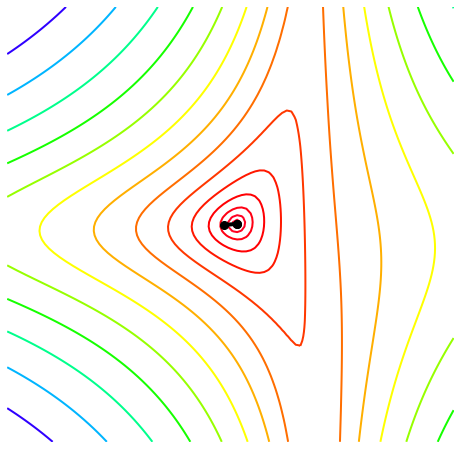
\includegraphics[width=0.18\linewidth]{newton/Lotka-Volterra/trapezoid_1.png}
        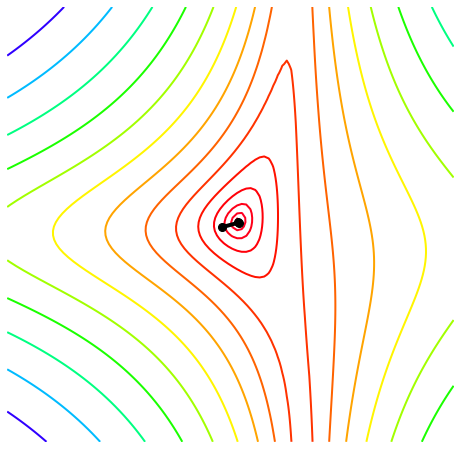
\includegraphics[width=0.18\linewidth]{newton/Lotka-Volterra/trapezoid_2.png}
        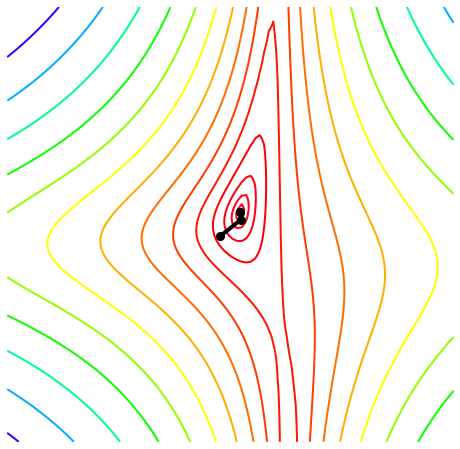
\includegraphics[width=0.18\linewidth]{newton/Lotka-Volterra/trapezoid_3.png}
        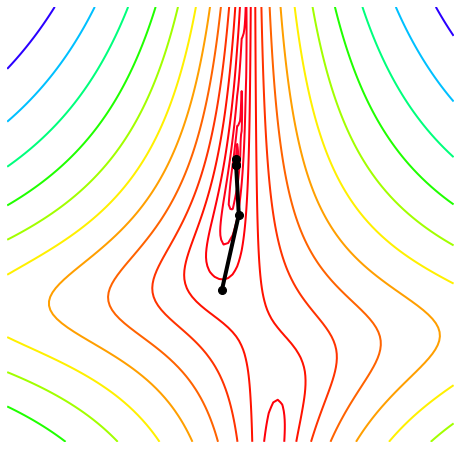
\includegraphics[width=0.18\linewidth]{newton/Lotka-Volterra/trapezoid_4.png}
        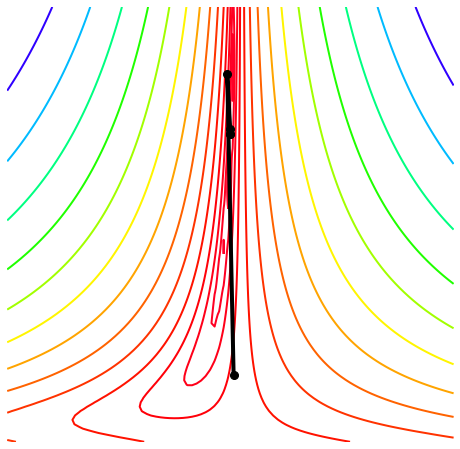
\includegraphics[width=0.18\linewidth]{newton/Lotka-Volterra/trapezoid_5.png}
        \\[4pt]
        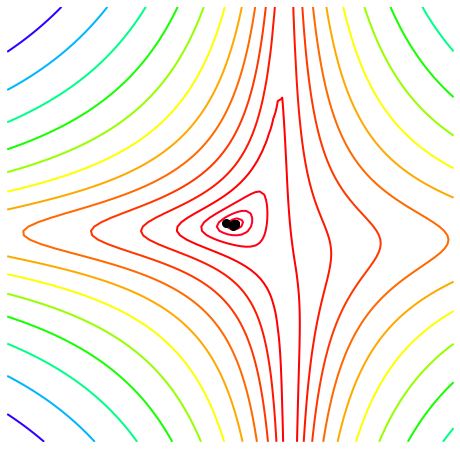
\includegraphics[width=0.18\linewidth]{newton/Lotka-Volterra/modeuler_1.png}
        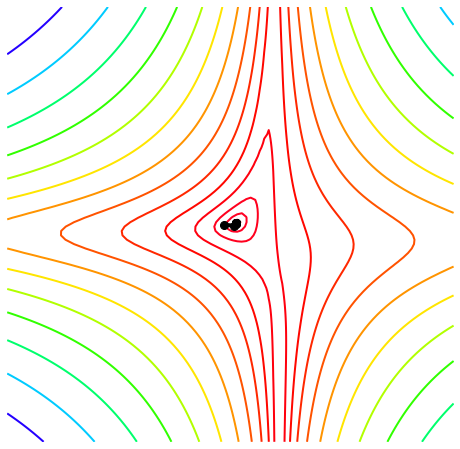
\includegraphics[width=0.18\linewidth]{newton/Lotka-Volterra/modeuler_2.png}
        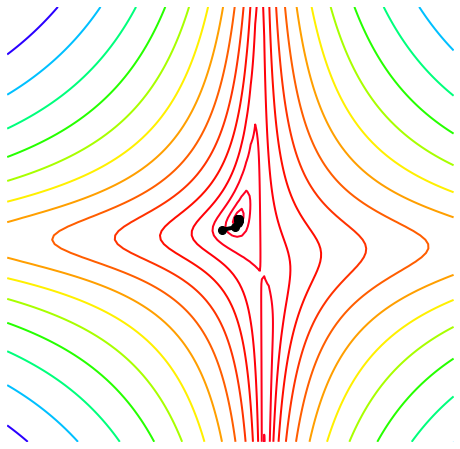
\includegraphics[width=0.18\linewidth]{newton/Lotka-Volterra/modeuler_3.png}
        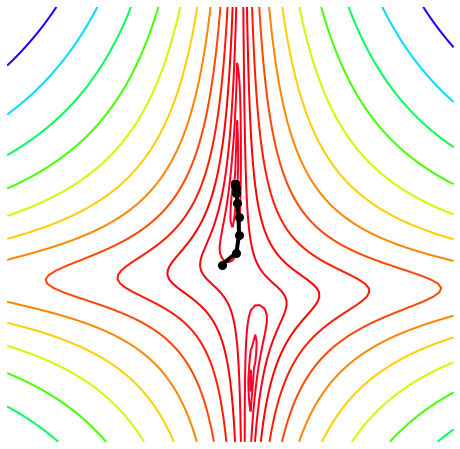
\includegraphics[width=0.18\linewidth]{newton/Lotka-Volterra/modeuler_4.png}
        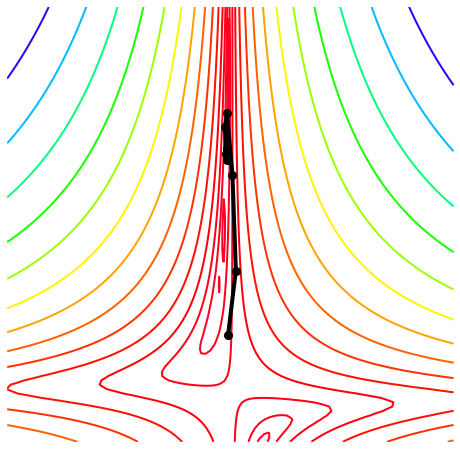
\includegraphics[width=0.18\linewidth]{newton/Lotka-Volterra/modeuler_5.png}
        \\[4pt]
        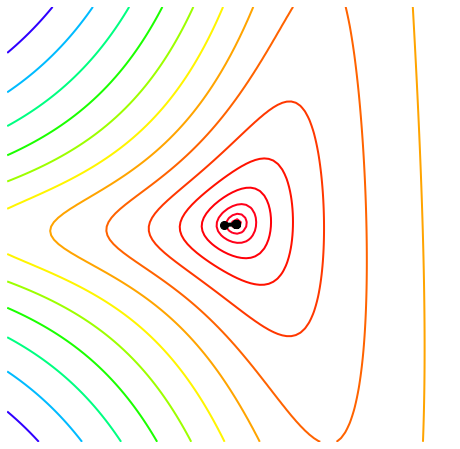
\includegraphics[width=0.18\linewidth]{newton/Lotka-Volterra/imex2_1.png}
        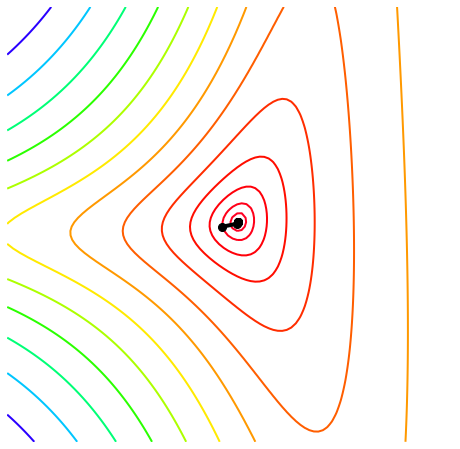
\includegraphics[width=0.18\linewidth]{newton/Lotka-Volterra/imex2_2.png}
        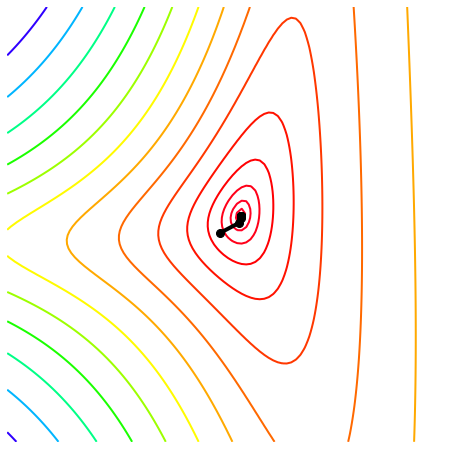
\includegraphics[width=0.18\linewidth]{newton/Lotka-Volterra/imex2_3.png}
        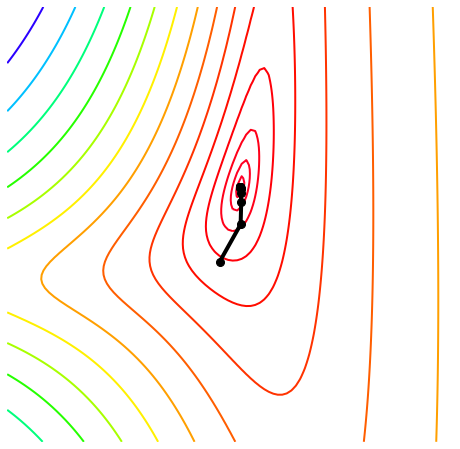
\includegraphics[width=0.18\linewidth]{newton/Lotka-Volterra/imex2_4.png}
        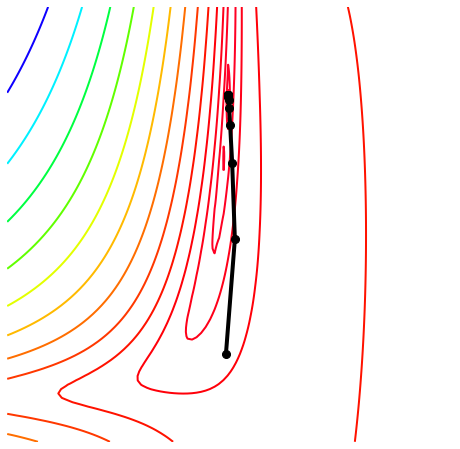
\includegraphics[width=0.18\linewidth]{newton/Lotka-Volterra/imex2_5.png}
	\end{center}
    \caption{Контуры $ 2 $-нормы невязки в зависимости от $ x \in [x^* - 15, x^* + 15] $ по горизонтали
        и $ y \in [y^* - 15, y^* + 15] $ по вертикали
        (где $ (x^*, y^*) $~--- центр траектории ньютоновских итераций)
        для метода трапеций (верхний ряд), Эйлера (модифицированный метод Ньютона) (средний ряд) и взвешенного метода Эйлера (нижний ряд)
        для пяти последовательных шагов по времени
        ($ \Delta t = 1 $), система Лотки-Вольтерры.
        Черная траектория соответствует итерациям Ньютона.
	}
	\label{fig:Lotka-Volterra_residual}
\end{figure}



\section{Осциллятор Ван дер Поля}
\label{sec:Van_der_Pol}

Жёсткая система, соответствующая уравнению Ван дер Поля \cite{alexander1991modified}, имеет вид
%
\begin{equation}
    \label{eq:Van_der_Pol}
    \varepsilon \frac{d x}{d t} = y - \left( \frac{1}{3} x^3 - x \right), \qquad \frac{d y}{d t} = -x
\end{equation}
Параметр $ \varepsilon $ регулирует жёсткость уравнения.
В данном эксперименте он положен равным $ 10^{-2} $.
Начальные условия: $ x_0 = 0.2 $, $ y_0 = 0 $.
Графики численных решений, а также зависимость числа потребовавшихся итераций метода Ньютона
от номера шага приведены на рисунке~\ref{fig:Van_der_Pol}.

\begin{sidewaysfigure}[!p]
    \centering
    \scriptsize
    \begin{gnuplot}[terminal=tikz, terminaloptions={color size 7.8cm,6.5cm fontscale 0.9}]
        small_plot = 1
        load './gnuplot/common.gp'

        set style data linespoints
        set xlabel  '$ t $'
        set xrange  [ 0 : * ] noreverse writeback
        set ylabel  '$ x(t) $' #rotate by 0
        set yrange  [ * : 4.2 ] noreverse writeback

        set xzeroaxis lw 2

        path = './data/nonlinear_stiffness/Van_der_Pol/120/'
        column = 3

        plot path.'implicit_euler.csv' every ::1 using 1:column t 'Неявный метод Эйлера', \
             path.'bdf2.csv' every ::1 using 1:column t 'формула дифф. назад 2-го порядка', \
             path.'modified_newton.csv' every ::1 using 1:column t 'модифицированный метод Ньютона' lc 'dark-plum', \
             path.'weighted_euler.csv' every ::1 using 1:column t 'взвешенный метод Эйлера' lc 'web-blue', \
             path.'reference.csv' every ::1 using 1:column with lines t 'референсное решение' ls 200
    \end{gnuplot}
    %
    \begin{gnuplot}[terminal=tikz, terminaloptions={color size 7.8cm,6.5cm fontscale 0.9}]
        small_plot = 1
        load './gnuplot/common.gp'

        set style data linespoints
        set xlabel  '$ t $'
        set xrange  [ 0 : * ] noreverse writeback
        set ylabel  '$ y(t) $' #rotate by 0
        set yrange  [ * : 1.5 ] noreverse writeback

        set xzeroaxis lw 2

        path = './data/nonlinear_stiffness/Van_der_Pol/120/'
        column = 4

        plot path.'implicit_euler.csv' every ::1 using 1:column t 'Неявный метод Эйлера', \
             path.'bdf2.csv' every ::1 using 1:column t 'формула дифф. назад 2-го порядка', \
             path.'modified_newton.csv' every ::1 using 1:column t 'модифицированный метод Ньютона' lc 'dark-plum', \
             path.'weighted_euler.csv' every ::1 using 1:column t 'взвешенный метод Эйлера' lc 'web-blue', \
             path.'reference.csv' every ::1 using 1:column with lines t 'референсное решение' ls 200
    \end{gnuplot}
    %
    \begin{gnuplot}[terminal=tikz, terminaloptions={color size 7.8cm,6.5cm fontscale 0.9}]
        small_plot = 1
        load './gnuplot/common.gp'

        set style data linespoints
        set xlabel  '$ t $'
        set xrange  [ 0 : * ] noreverse writeback
        set ylabel  '$ \niter(t) $' #rotate by 0
        set yrange  [ 0 : 250 ] noreverse writeback

        path = './data/nonlinear_stiffness/Van_der_Pol/120/'
        column = 2

        plot path.'modified_newton.csv' every ::1 using 1:column t 'модифицированный метод Ньютона' lc 'dark-plum', \
             path.'weighted_euler.csv' every ::1 using 1:column t 'взвешенный метод Эйлера' lc 'web-blue'
    \end{gnuplot}

    \begin{gnuplot}[terminal=tikz, terminaloptions={color size 7.8cm,6.5cm fontscale 0.9}]
        small_plot = 1
        load './gnuplot/common.gp'

        set style data linespoints
        set xlabel  '$ t $'
        set xrange  [ 0 : * ] noreverse writeback
        set ylabel  '$ x(t) $' #rotate by 0
        set yrange  [ * : 4.4 ] noreverse writeback

        set xzeroaxis lw 2

        path = './data/nonlinear_stiffness/Van_der_Pol/120/'

        plot path.'trapezoid.csv' every ::1 using 1:3 t 'метод трапеций', \
             path.'L_pareschi_russo.csv' every ::1 using 1:3 t 'L-устойчивый метод Парески-Руссо', \
             path.'qin_zhang.csv' every ::1 using 1:3 t 'метод Кина-Жанга', \
             path.'reference.csv' every ::1 using 1:3 with lines t 'референсное решение' ls 200
    \end{gnuplot}
    %
    \begin{gnuplot}[terminal=tikz, terminaloptions={color size 7.8cm,6.5cm fontscale 0.9}]
        small_plot = 1
        load './gnuplot/common.gp'

        set style data linespoints
        set xlabel  '$ t $'
        set xrange  [ 0 : * ] noreverse writeback
        set ylabel  '$ y(t) $' #rotate by 0
        set yrange  [ * : 1.5 ] noreverse writeback

        set xzeroaxis lw 2

        path = './data/nonlinear_stiffness/Van_der_Pol/120/'

        plot path.'trapezoid.csv' every ::1 using 1:4 t 'метод трапеций', \
             path.'L_pareschi_russo.csv' every ::1 using 1:4 t 'L-устойчивый метод Парески-Руссо', \
             path.'qin_zhang.csv' every ::1 using 1:4 t 'метод Кина-Жанга', \
             path.'reference.csv' every ::1 using 1:4 with lines t 'референсное решение' ls 200
    \end{gnuplot}
    %
    \begin{gnuplot}[terminal=tikz, terminaloptions={color size 7.8cm,6.5cm fontscale 0.9}]
        small_plot = 1
        load './gnuplot/common.gp'

        set style data linespoints
        set xlabel  '$ t $'
        set xrange  [ 0 : * ] noreverse writeback
        set ylabel  '$ \niter(t) $' #rotate by 0
        set yrange  [ 0 : 160 ] noreverse writeback

        path = './data/nonlinear_stiffness/Van_der_Pol/120/'

        plot path.'trapezoid.csv' every ::1 using 1:2 t 'метод трапеций', \
             path.'qin_zhang.csv' every ::1 using 1:2 t 'метод Кина-Жанга', \
             path.'L_pareschi_russo.csv' every ::1 using 1:2 t 'L-устойчивый метод Парески-Руссо'
    \end{gnuplot}

    \caption{Сравнение методов на примере интегрирования системы Ван дер Поля для шага по времени $ \Delta t = 0.05 $.}
    \label{fig:Van_der_Pol}
\end{sidewaysfigure}

Данная система является значительно жёсткой как в линейном, так и в нелинейном смысле.
Неявный метод Эйлера, формула дифференцирования назад второго порядка,
а также метод трапеций на некоторой итерации сошлись к физически некорректному корню.
Это является признаком нелинейной жёсткости.
Также метод трапеций регулярно показывал сильно осциллирующее поведение,
что говорит о значительной линейной жёсткости.
Оба предложенных метода в то же время дают корректные решения,
повторяющие динамику референсного решения, причём без нефизичных осцилляций.
Взвешенный метод Эйлера воспроизводит референсное решение без дисперсионной ошибки,
в то время как модифицированный метод Ньютона даёт несколько запаздывающие колебания.
Видно, однако, что модифицированный метод Ньютона почти всегда досрочно завершается из-за достижения предельного числа итераций.
Взвешенный метод Эйлера также в этом смысле сравнительно затратен, но задачу решает.

В сравнение также были включены \emph{L-устойчивый метод Парески-Руссо} \cite{pareschi2005imex} и \emph{метод Кина-Жанга} \cite{qin1992symplecticdirk}~---
два A-устойчивых диагонально-неявных двухстадийных метода Рунге-Кутты второго порядка аппроксимации,
задаваемых следующими таблицами Бутчера соответственно:
%
\begin{equation}
    \label{eq:Pareschi-Russo_and_Qin-Zhang}
    \begin{array}{c|cc}
        1 - \frac{\sqrt{2}}{2} & 1 - \frac{\sqrt{2}}{2} & 0 \\
        \frac{\sqrt{2}}{2}    & \sqrt{2} - 1          & 1 - \frac{\sqrt{2}}{2} \\
        \hline
         & \frac{1}{2} & \frac{1}{2}
    \end{array}
    \qquad \qquad
    \begin{array}{c|cc}
        1/4 & 1/4 & 0 \\
        3/4 & 1/2 & 1/4 \\
        \hline
         & 1/2 & 1/2
    \end{array}
\end{equation}
%
На графиках видно, что численные решения, полученные при помощи данных методов,
имеют нефизичные пики в окресности резких перепадов референсного решения.

На рисунке \ref{fig:Van_der_Pol_residual} приведены графики нормы невязки для метода трапеций,
модифицированного метода Ньютона и взвешенного метода Эйлера,
возникающие при решении нелинейных систем на некоторых пяти последовательных шагах
численного интегрирования системы Ван дер Поля.
Снова хорошо видна седловая структура задачи.
В случае метода трапеций и модифицированного метода Ньютона путь,
образуемый ньютоновскими итерациями, осциллирует между минимумами (см. третий столбец).
С другой стороны, взвешенный метод Эйлера избегает этой проблемы.

\begin{figure}[ht!]
	\begin{center}
        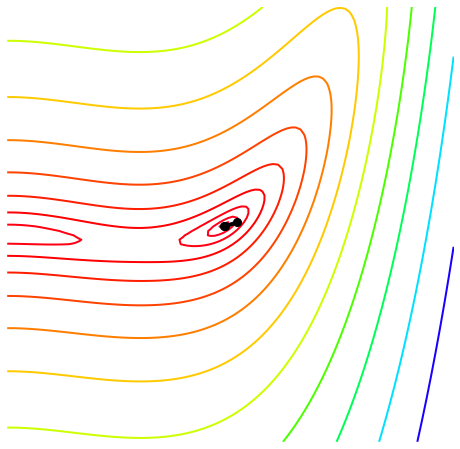
\includegraphics[width=0.18\linewidth]{newton/Van_der_Pol/trapezoid_1.png}
        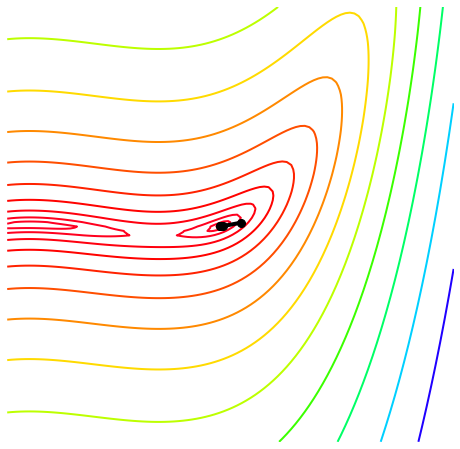
\includegraphics[width=0.18\linewidth]{newton/Van_der_Pol/trapezoid_2.png}
        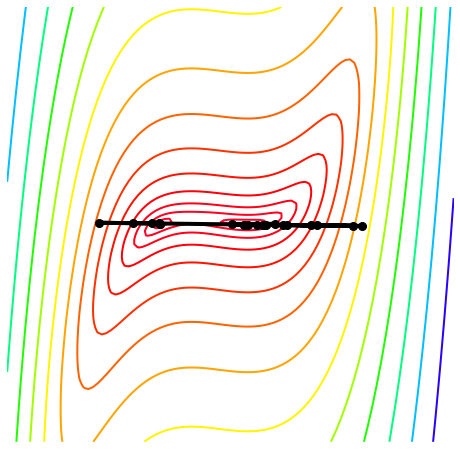
\includegraphics[width=0.18\linewidth]{newton/Van_der_Pol/trapezoid_3.png}
        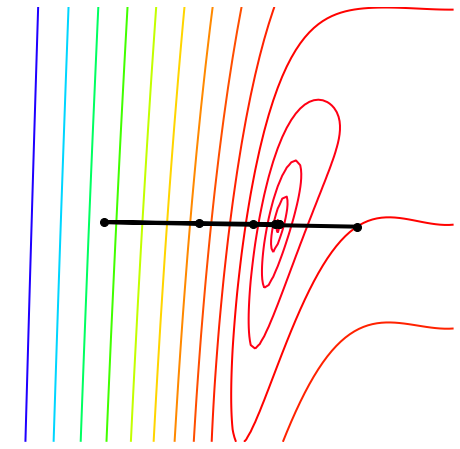
\includegraphics[width=0.18\linewidth]{newton/Van_der_Pol/trapezoid_4.png}
        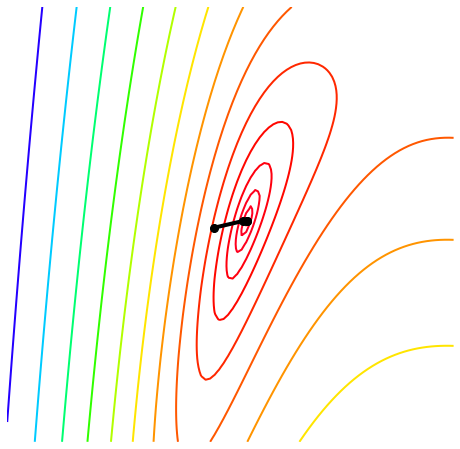
\includegraphics[width=0.18\linewidth]{newton/Van_der_Pol/trapezoid_5.png}
        \\[4pt]
        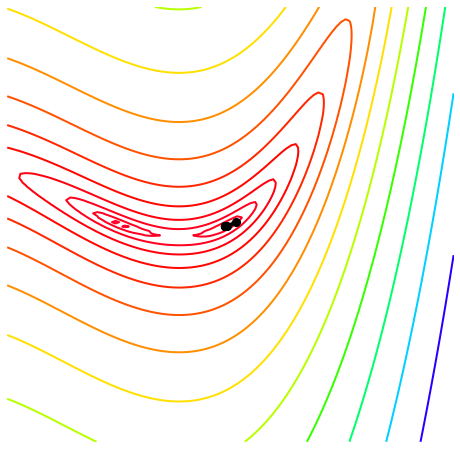
\includegraphics[width=0.18\linewidth]{newton/Van_der_Pol/modeuler_1.png}
        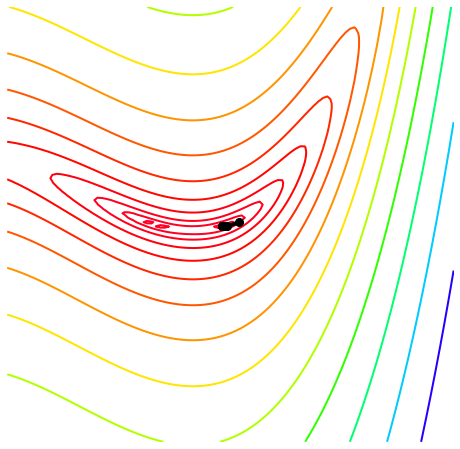
\includegraphics[width=0.18\linewidth]{newton/Van_der_Pol/modeuler_2.png}
        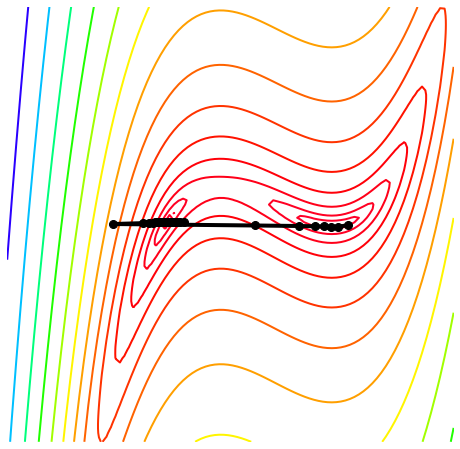
\includegraphics[width=0.18\linewidth]{newton/Van_der_Pol/modeuler_3.png}
        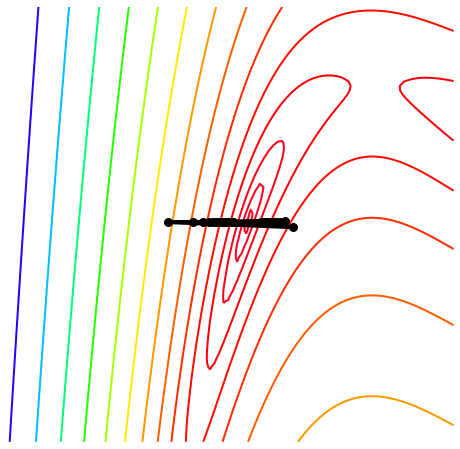
\includegraphics[width=0.18\linewidth]{newton/Van_der_Pol/modeuler_4.png}
        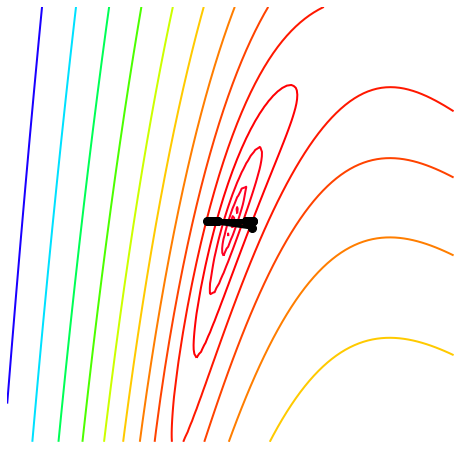
\includegraphics[width=0.18\linewidth]{newton/Van_der_Pol/modeuler_5.png}
        \\[4pt]
        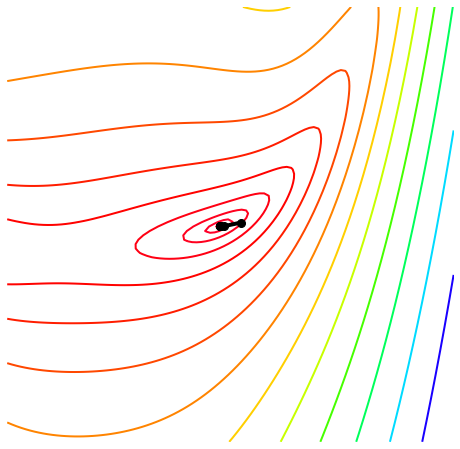
\includegraphics[width=0.18\linewidth]{newton/Van_der_Pol/imex2_1.png}
        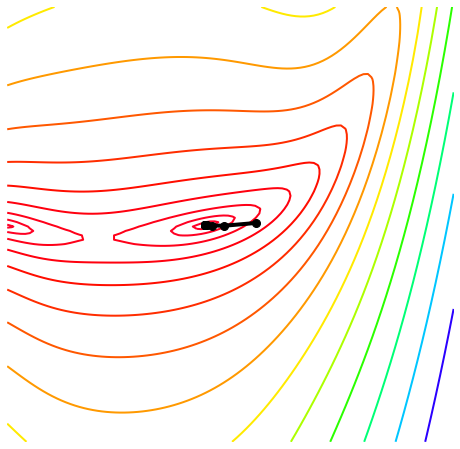
\includegraphics[width=0.18\linewidth]{newton/Van_der_Pol/imex2_2.png}
        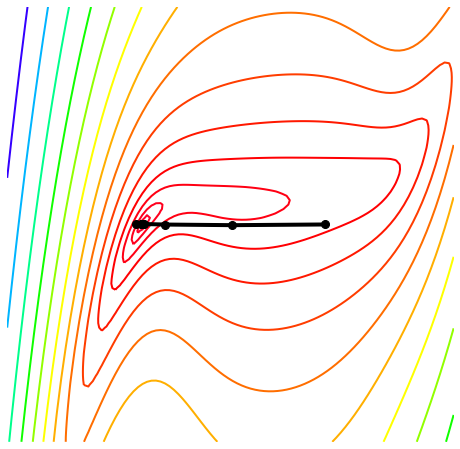
\includegraphics[width=0.18\linewidth]{newton/Van_der_Pol/imex2_3.png}
        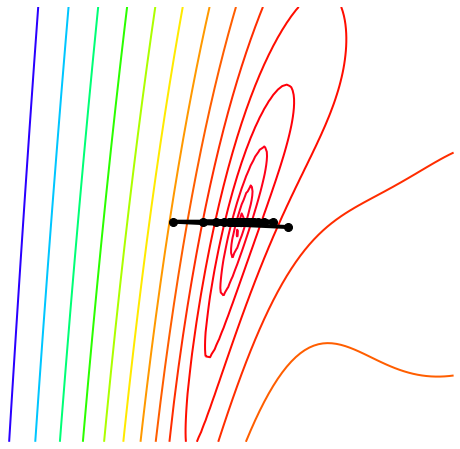
\includegraphics[width=0.18\linewidth]{newton/Van_der_Pol/imex2_4.png}
        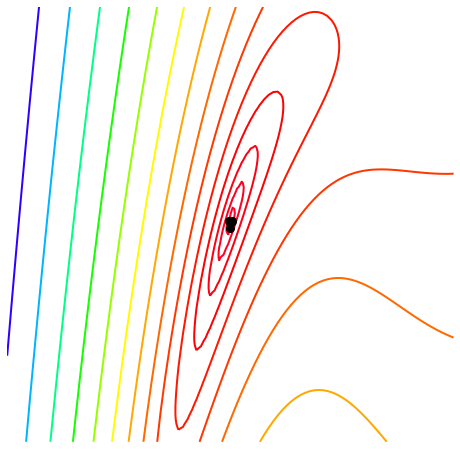
\includegraphics[width=0.18\linewidth]{newton/Van_der_Pol/imex2_5.png}
	\end{center}
    \caption{Контуры $ 2 $-нормы невязки в зависимости от $ x \in [x^* - 1.5, x^* + 1.5] $ по горизонтали
        и $ y \in [y^* - 1.5, y^* + 1.5] $ по вертикали
        (где $ (x^*, y^*) $~--- центр траектории ньютоновских итераций)
        для метода трапеций (верхний ряд), Эйлера (модифицированный метод Ньютона) (средний ряд) и взвешенного метода Эйлера (нижний ряд)
        для пяти последовательных шагов по времени
        ($ \Delta t = 0.1 $), осциллятор Ван дер Поля.
        Черная траектория соответствует итерациям Ньютона.
	}
	\label{fig:Van_der_Pol_residual}
\end{figure}



\section{Каскад свёртывания крови}
\label{sec:blood_coagulation_cascade}

Перейдём, наконец, к системе каскада свёртывания крови.
Данная система взята из~\cite{bouchnita2020mathematical, vassilevski2020parallel}
и является упрощённой моделью более подробного каскада свёртывания крови~\cite{panteleev2008coagulation, ushakova2018gemo}.
Уравнения модели приведены в~\eqref{eq:blood_coagulation_cascade}, начальные условия и параметры ~--- в таблице~\ref{tab:blood_coagulation_cascade}.
%
\begin{equation}
    \label{eq:blood_coagulation_cascade}
    \begin{aligned}
        \frac{\partial P}{\partial t} = - \left(k_1 \phi_c + k_2 B_\alpha + k_3 T + k_4 T^2 + k_5 T^3\right) P,
        \\
        \frac{\partial T}{\partial t} = \left(k_1 \phi_c + k_2 B_\alpha + k_3 T + k_4 T^2 + k_5 T^3 \right) P - k_6 A T,
        \\
        \frac{\partial B_\alpha}{\partial t} =  \left(k_7 \phi_c + k_8 T \right) \left( B^0 - B_\alpha \right) - k_9 A B_\alpha,
        \quad
        \frac{\partial A}{\partial t} = -k_6 A T - k_9 A B_\alpha,
        \\
        \frac{\partial F_g}{\partial t} = -\frac{k_{10} T F_g}{K_{10} + F_g},
        \quad
        \frac{\partial F}{\partial t} = \frac{k_{10} T F_g}{K_{10} + F_g} - k_{11} F,
        \quad
        \frac{\partial F_p} {\partial t} = k_{11} F,
        \\
        \frac{\partial \phi_c}{\partial t}  = - \left( k_{12} T - k_{13} \phi_c \right) \phi_f,
        \quad
        \frac{\partial \phi_f}{\partial t} = \left( k_{12} T - k_{13} \phi_c \right) \phi_f.
    \end{aligned}
\end{equation}

\begin{sidewaystable}[p!]
	%\footnotesize
	\centering

    \caption{Начальные условия и параметры модели (каскад свёртывания крови).}
	\label{tab:blood_coagulation_cascade}

	\begin{tabular}{cccccccc}
		\hline
		$ P $ & $ T $ & $ B_{\alpha} $ & $ A $ & $ F_g $ & $ F $ & $ F_p $ & $ \phi_c $  \\
		%\hline
		$ 1400 $ & $ 0 $ & $ 10 $ & $ 3400 $ & $ 7000 $ & $ 0 $ & $ 0 $ & $ 299 $  \\
		\hline
		 $ \phi_f $ & $ k_1 $ & $ k_2 $ & $ k_3 $ & $ k_4 $ & $ k_5 $ & $ k_6 $ & $ k_7 $   \\
		%\hline
		$ 1 $   & $ 1.5 \cdot 10^{-4} $ & $ 7.5 \cdot 10^{-6} $ & $ 1.5 \cdot 10^{-5} $ & $ 8 \cdot 10^{-6} $ & $ 10^{-10} $ & $ 4.817 \cdot 10^{-6} $ & $ 10^{-9} $ \\
		\hline
		$ k_8 $ & $ k_9 $ & $ k_{10} $ & $ K_{10} $ & $ k_{11} $ & $ k_{12} $ & $ k_{13} $ & $ B^0 $ \\
		%\hline
		 $ 5.2173 \cdot 10^{-5} $  & $ 2.223 \cdot 10^{-9} $ & $ 0.005 $ & $ 3160 $ & $ 0.1 $ & $ 0.002 $ & $ 4 \cdot 10^{-9} $ & $ 200 $ \\
		\hline
	\end{tabular}
\end{sidewaystable}

Результаты численного эксперимента можно найти в таблице \ref{tab:blood_coagulation_cascade_results}.
Время моделирования~--- $ T = 100 $.
Ошибка метода $ \mathcal{E}_x $ для переменной $ x(t) $ относительно референсного решения $ x_{ref}(t) $ вычислялась по формуле
%
\begin{equation}
    \label{eq:error_relative_to_reference}
	\mathcal{E}_x =\left. \sqrt{ T
		  \int\limits_{t \in [0,T] } \left( x(t) - x_{ref}(t) \right)^2 {\rm d} t
		}
		\middle/
		\int\limits_{t \in [0,T]} \left| x_{ref} (t) \right| {\rm d} t
		\right. .
\end{equation}
%
Полная ошибка метода вычислялась как среднеквадратическая ошибка по всем переменным.
В таблице также приведено полное $ \niter^{\text{общ}} $,
среднее $ \niter^{\text{сред}} $, минимальное $ \niter^{\text{мин}} $ и максимальное $ \niter^{\text{макс}} $ число потребовавшихся ньютоновских итераций.
Дополнительно указано число ньютоновских итераций, на которых решение оказывалось в отрицательной области~--- $ \niter^{\text{отриц}} $.

\begin{table}[ht!]
	\small
	\centering

    \caption{Результаты для модели каскада свёртывания крови.}
	\label{tab:blood_coagulation_cascade_results}

    \begin{tabular}{c|c|cccc|c|c}
        \hline
        Метод & $\Delta t$ &  $ \niter^{\text{общ}} $ & $ \niter^{\text{сред}} $ & $ \niter^{\text{мин}} $ & $ \niter^{\text{макс}} $ & $ \mathcal{E} $ &  $ \niter^{\text{отриц}} $ \\
        \hline
        Неявный Эйлера & $ 10^{-2} $         & $ 10812 $ & $ 1.0812 $  & $ 1 $ & $ 3 $   & $ 1.7 \cdot 10^{-2} $ & $ 0 $ \\
        Неявный Эйлера & $ 10^{-1} $         & $ 2032 $  & $ 2.032 $   & $ 2 $ & $ 5 $   & $ 0.17 $ & $ 0 $ \\
        Неявный Эйлера & $ 1 $               & $ 233 $   & $ 2.33 $    & $ 2 $ & $ 19 $  & $ 0.79 $ & $ 10 $ \\
        \hline
        Мод. Ньютона & $ 10^{-2} $ & $ 22071 $ & $ 2.20 $ & $ 2 $  & $ 7 $  & $ 1.7 \cdot 10^{-2} $ & $ 0 $ \\
        Мод. Ньютона & $ 10^{-1} $ & $ 3740 $  & $ 3.74 $ & $ 3 $  & $ 20 $ & $ 0.17 $ & $ 0 $ \\
        Мод. Ньютона & $ 1 $       & $ 768 $   & $ 7.68 $ & $ 4 $  & $ 53 $ & $ 0.79 $ & $ 10 $ \\
        Мод. Ньютона & $ 2 $       & $ 502 $   & $ 10.0 $ & $ 5 $  & $ 82 $ & $ 1.14 $ & $ 12 $ \\
        Мод. Ньютона & $ 5 $       & $ 240 $   & $ 12.0 $ & $ 9 $  & $ 26 $ & $ 1.19 $ & $ 13 $ \\
        Мод. Ньютона & $ 10 $      & $ 164 $   & $ 16.4 $ & $ 11 $ & $ 20 $ & $ 1.17 $ & $ 6 $ \\
        \hline
	    Трапеций & $ 10^{-2} $ & $ 10701 $  & $ 1.0701 $    & $ 1 $ & $ 3 $ & $ 1.6 \cdot 10^{-3} $ & $ 0 $ \\
		Трапеций & $ 10^{-1} $ & $ 2023 $  & $ 2.023 $    & $ 2 $ & $ 4 $ & $ 3.8 \cdot 10^{-2} $ & $ 0 $ \\
        \hline
        Взвешенный Эйлера & $ 10^{-2} $ & $ 10716 $ & $ 1.0716 $ & $ 1 $ & $ 3 $ & $ 1.6 \cdot 10^{-3} $ & $ 0 $ \\
        Взвешенный Эйлера & $ 10^{-1} $ & $ 2052 $  & $ 2.052 $  & $ 2 $ & $ 7 $ & $ 3.3 \cdot 10^{-2} $ & $ 0 $ \\
        Взвешенный Эйлера & $ 2.5 \cdot 10^{-1} $ & $ 861 $  & $ 2.1525 $    & $ 2 $ & $ 15 $ & $ 8.2 \cdot 10^{-2} $ & $ 3 $ \\
    \end{tabular}
\end{table}

Применение неявного метода Эйлера напрямую ведёт к нефизичному отрицательному решению для $ \Delta t \geqslant 2 $ (рис. \ref{fig:blood_coagulation}).
В то же время, модифицированный метод Ньютона позволил получить корректное решение для шагов вплоть до $ \Delta t = 10 $ включительно.
Использование метода трапеций с тем же шагом приводило к появлению сильно осциллирующих нефизичных осцилляций.
Взвешенный метод Эйлера позволил увеличить точность для маленьких шагов по времени ($ \Delta t \leqslant 0.25 $),
но при использовании больших шагов также получались решения с нефизичными осцилляциями
(пусть и заметно меньшими по амплитуде, чем у метода трапеций).

Из поведения численных методов снова можно сделать вывод,
что модель каскада свёртывания крови является жёсткой во всех предложенных смыслах.
При этом предложенные методы позволяют кратно увеличить шаг интегрирования данной системы без потери устойчивости.

\begin{figure}[ht!]
    \begin{center}
        \small
        \begin{gnuplot}[terminal=tikz, terminaloptions={color size 16.5cm,8.0cm fontscale 0.9}]
            load './gnuplot/common.gp'

            set style data linespoints
            set xlabel  '$ t $'
            set xrange  [ 0 : * ] noreverse writeback
            set ylabel  '$ T(t) $' offset -1 #rotate by 0
            set yrange  [ * : 2500 ] noreverse writeback

            set xzeroaxis lw 2

            path = './data/blood_coag/'

            plot path.'implicit_euler.csv' every ::1 using 1:3 t 'неявный метод Эйлера', \
                 path.'trapezoid.csv' every ::1 using 1:3 t 'метод трапеций', \
                 path.'modified_newton.csv' every ::1 using 1:3 t 'модифицированный метод Ньютона' lc 'dark-plum', \
                 path.'weighted_euler.csv' every ::1 using 1:3 t 'взвешенный метод Эйлера' lc 'web-blue', \
                 path.'reference.csv' every ::1 using 1:3 with lines t 'референсное решение' ls 200
        \end{gnuplot}

        \begin{gnuplot}[terminal=tikz, terminaloptions={color size 16.5cm,8.0cm fontscale 0.9}]
            load './gnuplot/common.gp'

            set style data linespoints
            set xlabel  '$ t $'
            set xrange  [ 0 : * ] noreverse writeback
            set ylabel  '$ F(t) $' offset -1 #rotate by 0
            set yrange  [ * : 700 ] noreverse writeback

            set xzeroaxis lw 2

            path = './data/blood_coag/'

            plot path.'implicit_euler.csv' every ::1 using 1:7 t 'неявный метод Эйлера', \
                 path.'trapezoid.csv' every ::1 using 1:7 t 'метод трапеций', \
                 path.'modified_newton.csv' every ::1 using 1:7 t 'модифицированный метод Ньютона' lc 'dark-plum', \
                 path.'weighted_euler.csv' every ::1 using 1:7 t 'взвешенный метод Эйлера' lc 'web-blue', \
                 path.'reference.csv' every ::1 using 1:7 with lines t 'референсное решение' ls 200
        \end{gnuplot}
    \end{center}
    \caption{Сравнение методов на примере интегрирования системы каскада свёртывания крови для шага по времени $ \Delta t = 10 $.
        Приведены графики зависимости концентрации тромбина (верх) и фибриногена (низ) от времени.}
    \label{fig:blood_coagulation}
\end{figure}

  %% Эксперименты.
    \chapter{Модель образования белого тромба}
\label{chapter:blood} \index{Модель}

\section{Модели распределения тромбоцитов в объёме}
\label{section:volume_distribution_models}

%При моделировании слипания тромбоцитов и механических свойств слипшейся массы разумно отказаться от феноменологического подхода
%и получить необходимые законы из вспомогательных теоретических результатов.
%В перспективе это может позволить уменьшить число параметров модели,
%сделать их более интерпретируемыми.

%В основе слипания тромбоцитов и роста вязкости тромба лежит связывание тромбоцитов
%сетью из развёрнутых молекул фактора фон Виллебранда, длина которых 

Распределение тромбоцитов в объёме напрямую влияет на формирование связей между ними,
что сказывается как на механических свойствах слипшейся массы, так и на скорости слипания.
Отсюда следует важность отдельного моделирования объёмного распределения тромбоцитов.

В данном разделе рассматривается вывод закона распределения из небольшого числа интуитивно понятных предположений.
Во-первых, предполагается, что при достижении предельной концентрации взаимное расположение тромбоцитов
близко к плотной упаковке трёхмерных шаров.
Во-вторых, считается, что при малых концентрациях тромбоциты распределены по объёму почти равномерно и случайно,
их взаимодействие между собой несущественно.
В-третьих, предполагается существование для средних значений концентрации переходного режима,
в котором распределение тромбоцитов всё еще достаточно случайное,
но взаимодействием между ними пренебрегать уже нельзя в силу значительности занимаемого ими объёма.


\subsection{Случай высокой концентрации}
\label{subsection:volume_distribution_models:high_concentration}

Высокая концентрация соответствует сформировавшемуся тромбу.
Тромбоциты в таком тромбе прилегают друг другу плотно.
В приближении сферически симметричных тромбоцитов
можно задействовать известный результат для плотной упаковки трёхмерных шаров:

\begin{theorem}[Гаусс, Кеплер, Хейлз~\cite{hales2002overview_kepler}]
    \label{theorem:high_concentration:packed_balls}
    В пространстве $ \reals^3 $ рассмотрим последовательность ограниченных измеримых множеств $ S_n $ таких,
    что $ n $-ое множество содержит шар радиуса хотя бы $ n $.
    Пусть $ \setfamily_n $~--- семейство подмножеств $ S_n $,
    являющихся дизъюнктным объединением единичных шаров.
    Пусть $ \varphi \colon \bigcup_{n \in \naturals} \setfamily_n \to \naturals_0 $
    отображает дизъюнктное объединение шаров в число шаров в этом объединении.
    Тогда
    \[
        \lim_{n \to \infty} \max_{R \in \setfamily_n} \frac{\varphi(R)}{\mu(S_n)} = \frac{\pi}{3 \sqrt{2}}
    \]
\end{theorem}

Таким образом, максимально возможная концентрация частиц радиуса $ R $ равна
\[
    n_\textnormal{max} = \frac{\pi}{3 \sqrt{2}} \cdot \frac{1}{\frac{4}{3} \pi R^3}
    = \frac{1}{4 \sqrt{2} R^3}
    = \frac{\sqrt{2}}{(2R)^3}
\]
Размер тромбоцитов в человеческой крови составляет примерно
$ 3 - 4 $ мкм~\cite{rumbaut2010platelets-vessel_interactions}.
Приняв этот размер за диаметр, получаем значение предельной концентрации:
от $ 2 \cdot 10^{16} \; \textnormal{м}^{-3} $ до $ 6 \cdot 10^{16} \; \textnormal{м}^{-3} $,
или примерно $ 40 \cdot 10^6 \; \textnormal{мкл}^{-1} $.
При нормальных условиях концентрация тромбоцитов в крови человека примерно равна
$ 0.3 \cdot 10^6 \; \textnormal{мкл}^{-1} $~\cite{zhang2022COPD_risk},
что более чем в $ 100 $ раз меньше предельной концентрации
(или, иначе говоря, среднее расстояние между тромбоцитами примерно в $ \sqrt[3]{100} \approx 5 $ раз больше их радиуса).

Таким образом, можно вполне справедливо полагать,
что на ранних этапах образования тромба концентрация тромбоцитов достаточно мала.


\subsection{Случай низкой концентрации}
\label{subsection:volume_distribution_models:low_concentration}

Рассмотрим сосуд объёма $ V_0 $,
наполненный жидкостью с равномерно распределённой примесью концентрации $ n = N / V_0 $.
Число частиц в части сосуда объёма $ V $ распределено биномиально с параметром $ p = V n / N = V / V_0 $:
\[
    \proba\{ \textnormal{\# частиц} = k \} = \binom{N}{k} \left(\frac{V}{V_0}\right)^k \left(1 - \frac{V}{V_0} \right)^{N-k}
\]
При устремлении $ V_0 / V \to +\infty $ получаем известный результат~---
распределение Пуассона для числа частиц в малом объёме:
%
\begin{multline*}
    \proba\{ \textnormal{\# частиц} = k \} \sim \frac{N^k}{k!} \left( \frac{V}{V_0} \right)^k \left( 1 - \frac{V}{V_0} \right)^N = \\ =
    \frac{(V_0 n)^k}{k!} \left( \frac{V}{V_0} \right)^k \left( 1 - \frac{V}{V_0} \right)^{V_0 n} \sim \frac{(V n)^k}{k!} e^{- V n} 
\end{multline*}
%
Заметим, что вероятность обнаружить в объёме $ V $ не менее $ k $ частиц равна
%
\begin{multline}
    \label{eq:low_concentration:volume_distribution}
    \proba\{ \textnormal{\# частиц} \geqslant k \} =
    1 - \proba\{ \textnormal{\# частиц} < k \} =
    1 - \sum_{m = 0}^{k-1} \proba\{ \textnormal{\# частиц} = m \} = \\ =
    1 - e^{- V n} \sum_{m = 0}^{k-1} \frac{(V n)^m}{m!}
\end{multline}
%
Полученное выражение является функцией распределения для
\emph{гамма"=распределения} с параметрами $ k $, $ 1/n $.

Нас интересует вероятностное распределение расстояния от выбранной частицы до $ k $-ого ближайшего соседа
(обозначим это расстояние $ r_k $).
То есть, что эквивалентно, вероятностное распределение объёма шара,
в котором есть хотя бы $ k $ частиц (помимо центра).

Обозначим $ V(r) $ и $ S(r) $~--- объём шара и площадь сферы радиуса $ r $ соответственно
(в трёхмерном случае~--- $ \frac{4}{3} \pi r^3 $ и $ 4 \pi r^2 $ соответственно).
%
\begin{equation}
    \label{eq:low_concentration:kNN-volume_equvalence}
    \proba\{r_k < x\} = \proba \left\{\textnormal{в $ V = V(x) $ находится $ \geqslant k $ частиц} \right\}
\end{equation}
%
Комбинируя~\eqref{eq:low_concentration:volume_distribution} и \eqref{eq:low_concentration:kNN-volume_equvalence},
получаем функцию распределения для $ r_k $:
%
\begin{equation}
    \label{eq:low_concentration:kNN_distance_CDF}
    F_{r_k}(x) = 1 - e^{- V(x) n} \sum_{m = 0}^{k-1} \frac{(V(x) n)^m}{m!}
\end{equation}
%
Дифференцируя по $ x $ (с учётом соотношения $ \partial V(x) / \partial x = S(x) $),
получаем плотность распределения:
%
\begin{multline}
    \label{eq:low_concentration:kNN_distance_PDF}
    \rho_{r_k}(x) = e^{-V(x) n} \cdot \left[ S(x) n \sum_{m = 0}^{k-1} \frac{(V(x) n)^m}{m!} -
    \sum_{m = 1}^{k-1} \frac{S(x) n (V(x) n)^{m-1}}{(m-1)!} \right] = \\ =
    S(x) n \cdot e^{-V(x) n} \frac{(V(x) n)^{k-1}}{(k-1)!}
\end{multline}
%
Характерный вид $ F_{r_k}(x) $ и $ \rho_{r_k}(x) $ представлен
на рисунке~\ref{fig:low_concentration:kNN_distance_distribution_plots}.

\begin{figure}[ht!]
    \centering
    \begin{subfigure}[t]{0.5\textwidth}
        \centering
        \captionsetup{aboveskip=-\baselineskip}
        \begin{gnuplot}[terminal=tikz, terminaloptions={color size 8.0cm,5.0cm fontscale 0.8}]
            load "./gnuplot/common.gp"
            load "./gnuplot/kNN_distribution.gp"

            set yrange [0:1]

            f_1(x)  = F_r(x,3,1)
            f_4(x)  = F_r(x,3,4)
            f_10(x) = F_r(x,3,10)

            plot [0:3] f_1(x) lw 2 t "$ F_{r_1}(x) $", \
                       f_4(x) lw 2 t "$ F_{r_4}(x) $", \
                       f_10(x) lw 2 t "$ F_{r_{10}}(x) $"
        \end{gnuplot}
        \caption{Функции распределения $ F_{r_k}(x) $.}
    \end{subfigure}%
    \begin{subfigure}[t]{0.5\textwidth}
        \centering
        \captionsetup{aboveskip=-\baselineskip}
        \begin{gnuplot}[terminal=tikz, terminaloptions={color size 8.0cm,5.0cm fontscale 0.8}]
            load "./gnuplot/common.gp"
            load "./gnuplot/kNN_distribution.gp"

            f_1(x)  = rho_r(x,3,1)
            f_4(x)  = rho_r(x,3,4)
            f_10(x) = rho_r(x,3,10)

            plot [0:3] f_1(x) lw 2 t "$ \\rho_{r_1}(x) $", \
                        f_4(x) lw 2 t "$ \\rho_{r_4}(x) $", \
                        f_10(x) lw 2 t "$ \\rho_{r_{10}}(x) $"
        \end{gnuplot}
        \caption{Функций плотности вероятности $ \rho_{r_k}(x) $.}
    \end{subfigure}
    \caption{Графики распределения случайной величины $ r_k $ для $ k \in \{1, 4, 10 \} $.}
    \label{fig:low_concentration:kNN_distance_distribution_plots}
\end{figure}


% В общем случае объём и площадь поверхности $ d $-мерного шара равны, соответственно,
% \begin{equation}
%     \label{eq:volume_distribution_models:d-dim_ball_volume_and_surface}
%     V_d(r) = \frac{\pi^{d/2}}{\Gamma(d/2 + 1)} \cdot r^d \qquad S_d(r) = 2 \pi V_{d-1}(r)
% \end{equation}
% Отсюда имеем
% \[
%     r = \frac{1}{\sqrt{\pi}} \left[ \Gamma(d/2+1) V_d(r) \right]^{1/d},
% \]
Найдём моменты случайной величины $ r_k $.
Вспомним, что объём $ d $-мерного шара радиуса $ r $ пропорционален $ r^d $:
\[
    V_d(r) = V_d(1) \cdot r^d \quad \Longrightarrow \quad r = \sqrt[d]{V_d(r) / V_d(1)},
\]
Тогда
%
\begin{align}
    \label{eq:low_concentration:kNN_distance_expectation}
    \expect r_k^m &= \int\limits_0^{+\infty} x^m \rho_{r_k}(x) \, dx =
    \int\limits_0^{+\infty} x^m e^{-V(x) n} \frac{(V(x) n)^{k-1}}{(k-1)!} \, S(x) n \, dx = \\
    &= \int\limits_0^{+\infty} x^m(V) \cdot e^{-V n} \frac{(V n)^{k-1}}{(k-1)!} \, d(V n) = \\
    &= V(1)^{-m/d} \int\limits_0^{+\infty} V^{m/d} \cdot e^{-V n} \frac{(V n)^{k-1}}{(k-1)!} \, d(V n) = \\
    &= \frac{(V(1) n)^{-m/d}}{(k-1)!} \int\limits_0^{+\infty} z^{m/d + k - 1} e^{-z} dz
    = \frac{\Gamma(m/d + k)}{\Gamma(k)} (V(1) n)^{-m/d}
\end{align}
В частности, в трёхмерном случае среднее расстояние до ближайшего соседа примерно равно $ 0.83 \cdot n^{-1/3} $.

% \begin{figure}
%     \centering
%     \begin{subfigure}[t]{0.5\textwidth}
%         \centering
%         \begin{gnuplot}[terminal=tikz, terminaloptions={color size 8.5cm,5.0cm}]
%             load "./gnuplot/common.gp"
%             load "./gnuplot/kNN_distribution.gp"
% 
%             set yrange [0:1]
% 
%             f_1(x)  = F_r_normalized(x,3,1)
%             f_4(x)  = F_r_normalized(x,3,4)
%             f_10(x) = F_r_normalized(x,3,10)
% 
%             plot [-3:3] f_1(x) lw 2 t "$ F_{r_1}(x) $", \
%                         f_4(x) lw 2 t "$ F_{r_4}(x) $", \
%                         f_10(x) lw 2 t "$ F_{r_{10}}(x) $"
%         \end{gnuplot}
%         \caption{Характерный вид функций распределения $ F_{r_k}(x) $.}
%     \end{subfigure}%
%     \begin{subfigure}[t]{0.5\textwidth}
%         \centering
%         \begin{gnuplot}[terminal=tikz, terminaloptions={color size 8.5cm,5.0cm}]
%             load "./gnuplot/common.gp"
%             load "./gnuplot/kNN_distribution.gp"
% 
%             f_1(x)  = rho_r_normalized(x,3,1)
%             f_4(x)  = rho_r_normalized(x,3,4)
%             f_10(x) = rho_r_normalized(x,3,10)
% 
%             plot [-3:3] f_1(x) lw 2 t "$ \\rho_{r_1}(x) $", \
%                         f_4(x) lw 2 t "$ \\rho_{r_4}(x) $", \
%                         f_10(x) lw 2 t "$ \\rho_{r_{10}}(x) $"
%         \end{gnuplot}
%         \caption{Характерный вид плотности распределения $ \rho_{r_k}(x) $.}
%     \end{subfigure}
% \end{figure}


\section{Модели образования белого тромба}
\label{section:blood:white_clot_model}

В данном разделе будет предложена модель образования белого тромба,
дополняющие результаты работ~\cite{bouchnita2020mathematical, vassilevski2020parallel}.
Основу модели будут составлять две компоненты: свободные, липкие и закрепившиеся тромбоциты.
Первые два компартмента будут моделироваться пассивной примесью,
третий будет образовывать неподвижную пористую среду.
Реакционная часть модели позволит описать переход тромбоцитов из одного компартмента в другой
под действием слипания и разъединения потоком.
Модели вязкости и проницаемости слипшейся массы должны позволить воспроизвести наблюдаемые процессы закрепления тромба
и блокировки потока крови.

Программная имплементация основана на конечно-объемном коде
уравнения переноса-диффузии-реакции из работы~\cite{vassilevski2020parallel},
позволяющем модифицировать реакционную часть,
отключать перенос определённых примесей,
а также динамически менять вязкость и проницаемость среды.
Поэтому в настоящем разделе мы сфокусируемся только на существенных модификациях,
вносимых в используемую модель.
Конкретно, будут описаны новые реакционные члены, а также модель вязкости и проницаемости.

\subsection{Реакционная часть}
\label{subsection:white_clot_model:reactions}

Традиционно процесс образования белого тромба описывается
многокомпонентной моделью~\cite{sorensen1999platelets_deposition_model, goodman2005thrombosis_model, taylor2016thrombosis_model, wu2017deposition_model}.
Однако экспериментальные данные позволяют предположить,
что воспроизведение отдельно механизма слипания тромбоцитов может потребовать добавления
лишь небольшого числа новых компонент в существующую модель фибринового тромба.

Результаты лабораторных опытов говорят о том,
что в областях повышенных сдвиговых напряжений происходят качественные изменения тромбоцитов,
заставляющие их налипать на стенку ниже по течению,
где сдвиговое напряжение возвращается к нормальному значению~\cite{rahman2019platelet_adhesion}.
Также известно, что сдвиговое напряжение влияет и на местную агрегацию тромбоцитов:
при его повышении фибриновые и фибриногеновые связи наблюдаются реже,
а связи посредством фактора фон Виллебранда~--- чаще~\cite{savage1996platelet_adhesion}.
Такое поведение связано с механическими свойствами фактора фон Виллебранда:
при малых скоростях сдвига фактор свёрнут в глобулу
и не может сцеплять тромбоциты между собой и со стенкой,
однако высокое сдвиговое напряжение позволяют глобулам развернуться,
что приводит к агрегации тромбоцитов~\cite{lippok2016vWF_unfolding, zhussupbekov2021vWF_unfolding}.

Можно выдвинуть предположение,
что в областях с повышенным сдвиговым напряжением тромбоциты образуют липкие агрегаты,
скреплённые частично или полностью развёрнутым фактором фон Виллебранда.
Агрегаты могут далее оседать как в месте образования, так и ниже по течению.
Такая модель требует введения всего двух компонент:
концентрации липких и слипшихся тромбоцитов.
Требуется также учесть разрушение связей между тромбоцитами из-за механического воздействия
или других факторов.
Итоговые уравнения имеют вид
%
\begin{equation}
    \label{eq:reactions:general_reactions_equations}
    \begin{dcases}
        \frac{\partial \phi_f}{\partial t} &= -k_{f \to a} \cdot \phi_f + k_{\textnormal{da}} \cdot \phi_a \\
        \frac{\partial \phi_a}{\partial t} &=  k_{f \to a} \cdot \phi_f - k_{a \to d} \cdot \phi_a + k_{\textnormal{da}} \cdot (\phi_d - \phi_a) \\
        \frac{\partial \phi_d}{\partial t} &=  k_{a \to d} \cdot \phi_a - k_{\textnormal{da}} \cdot \phi_d \\
    \end{dcases}
\end{equation}
%
где $ \phi_f $, $ \phi_a $ и $ \phi_d $~--- концентрации свободных, липких и слипшихся тромбоцитов соответственно,
$ k_\textnormal{da} $~--- скорость дизагрегации тромбоцитов из-за внешнего воздействия,
а $ k_{f \to a} $ и $ k_{a \to d} $ отвечают за скорость агрегации и слипания тромбоцитов.
Концентрации $ \phi_f $ и $ \phi_a $ участвуют в переносе и диффузии в качестве пассивной примеси,
$ \phi_d $ же считается концентрацией строго неподвижной примеси.

Будем рассматривать случай высоких сдвиговых напряжений,
когда большая часть связей между тромбоцитами опосредована фактором фон Виллебранда.
В работе~\cite{savage1996platelet_adhesion} представлены данные,
описывающие динамику налипших на подложку с фактором фон Виллебранда тромбоцитов
с течением времени и при разных сдвиговых напряжениях.
Из них можно сделать вывод, что $ k_\text{da} $ почти не зависит от сдвигового напряжения
(что не так для фибрина и фибриногена) и примерно равен $ 3.3 \cdot 10^{-2} \; \text{с}^{-1} $.

Из той же работы также можно получить зависимость $ k_{f \to a} $ и $ k_{a \to d} $ от сдвигового напряжения,
которая должна быть пропорциональна предельному числу налипших на подложку тромбоцитов
%(рисунок 2 в~\cite{savage1996platelet_adhesion} и рисунок~\ref{fig:reactions:vWF_platelets_count}).
(рисунок~\ref{fig:reactions:vWF_platelets_count}).


\begin{figure}[ht!]
    \centering
    \small
    \begin{gnuplot}[terminal=tikz, terminaloptions={color size 16.0cm,8.0cm fontscale 0.8}]
        load './gnuplot/common.gp'

        set datafile separator ' '

        set style increment default
        set style data lines
        set xlabel  "$ \\dot \\gamma $"
        set xrange  [ 0 : 1600 ] noreverse writeback
        set ylabel  "$ N_\\textnormal{platelets} $" offset -1 #rotate by 0
        set yrange  [ * : 1000 ] noreverse writeback

        # Модель
        f(x) = 805.7 * (1.0 - 0.759 * exp(-2.845e-3 * x))

        set xtics 100
        #set xzeroaxis lw 2

        plot "./data/platelets/Savage_data.csv" using 1:3 with points ps 3 t "экспериментальные данные \\cite{savage1996platelet_adhesion}", \
             f(x) with lines lw 3 t "модель \\eqref{eq:reactions:vWF_shear_model}"
    \end{gnuplot}
    \caption{Зависимость числа налипших тромбоцитов от сдвигового напряжения в потоке у стенки~\cite{savage1996platelet_adhesion}.}
    \label{fig:reactions:vWF_platelets_count}
\end{figure}

Решая задачу наименьших квадратов с экспоненциальной моделью, получаем
%
\begin{equation}
    \label{eq:reactions:vWF_shear_model}
    k_{f \to a}, \; k_{a \to d} \sim 1 - a \, e^{-b \, \dot{\gamma}},
    \qquad
    a = 0.76, \;
    b = 2.85 \cdot 10^{-3} \; \textnormal{с},
\end{equation}
%
где $ \dot{\gamma} $~--- скорость сдвига.

В работе~\cite{wu2017deposition_model} предлагается считать процесс формирования тромба послойным,
то есть переход $ \phi_a \to \phi_d $ возможен только вблизи поверхности сосуда или уже образовавшегося тромба.
Математически данная идея формализуется посредством свёртки некоторого ядра $ K(\vec{r}) $,
ширина которого отвечает за характерное расстояние слипания тромбоцитов,
с функцией $ \alpha_c \cdot \phi_d(\vec{r}) + \alpha_b \cdot \indicator_{\partial \Omega_{\textnormal{adh}}}(\vec{r}) $,
где $ \partial \Omega_\textnormal{adh} $ обозначает границу области, на которую могут крепиться тромбоциты,
а коэффициенты $ \alpha $ регулируют скорость налипания.

На практике расстояния, на которых формируются связи между тромбоцитами,
гораздо меньше характерных размеров ячеек расчётной сетки,
а потому результат свёртки будет равен $ \alpha_c \cdot S_d + \alpha_b \cdot S_b $,
где $ S_b $~--- суммарная площадь контакта ячейки с той частью границы, на которую могут крепиться тромбоциты,
а $ S_c $~--- суммарная площадь контакта с соседними ячейками, в которых тромб уже сформирован.
В работе~\cite{wu2017deposition_model} предлагается следующая формула для $ S_c $:
\[
    S_c(\mathrm{c}) = \sum_{\mathrm{f} \in \textnormal{faces}(\mathrm{c})} |\mathrm{f}| \cdot
    (\phi_d(\mathrm{f}) / \phi_{\max}) \cdot \indicator_{[\phi_\textnormal{clot}; +\infty)}(\phi_d(\mathrm{f})),
\]
где $ \mathrm{c} $~--- рассматриваемая ячейка,
%$ |\mathrm{c}| $~--- объём ячейки $ \mathrm{c} $,
$ \textnormal{faces}(\mathrm{c}) $~--- грани ячейки $ \mathrm{c} $,
$ |\mathrm{f}| $~--- площадь грани $ \mathrm{f} $,
$ \phi_d(\mathrm{f}) $~--- концентрация $ \phi_d $
в ячейке через грань $ \mathrm{f} $ от $ \mathrm{c} $,
$ \phi_{\max} $~--- максимально допустимая концентрация тромбоцитов
(см.~\ref{subsection:volume_distribution_models:high_concentration}),
а $ \phi_{\textnormal{clot}} $~--- минимальная концентрация тромбоцитов в белом тромбе
(определяется экспериментально).


\subsection{Модель вязкости}
\label{subsection:white_clot_model:viscocity}

В работе~\cite{jamiolkowski2016visualization} было продемонстрировано,
что белый тромб ведёт себя как вязкопластичная среда,
вязкость которой растёт по мере роста концентрации за счёт образования новых связей между тромбоцитами.
Пренебрегая пластичным аспектом,
построим модель вязкости тромба из предположения о её пропорциональности числу связей между липкими ($ \phi_a $) тромбоцитами;
связи между уже слипшимися и закрепившимися тромбоцитами не рассматриваются, так как последние формируют неподвижную массу,
не участвующую в переносе и диффузии.

Микрофотографии, приведённые в работе~\cite{schneider2007vWF_unfolding},
говорят о том, что агрегация тромбоцитов посредством
фактора фон Виллебранда может наблюдаться на расстоянии до $ 10 - 15 \; \text{мкм} $;
обозначим данное характерное расстояние за $ L_\textnormal{vWF} $ .
При этом можно предполагать, что сравнительно устойчивые агрегаты формируются только тогда,
когда каждый тромбоцит сцеплен с тремя или более другими тромбоцитами.
Тогда можно рассмотреть следующую модель вязкости:
%
\begin{equation}
    \label{eq:viscocity:viscocity_model}
    \nu = \nu_0 \cdot (1 + \beta \cdot F_{r_k}(L_\textnormal{vWF})),
\end{equation}
%
где $ \nu_0 $~--- вязкость крови без агрегаций из тромбоцитов,
$ F_{r_k} $ определена в уравнении~\eqref{eq:low_concentration:kNN_distance_CDF},
$ \beta $~--- параметр влияния степени агрегации тромбоцитов на вязкость,
$ k \approx 4 $, $ L_\textnormal{vWF} \approx 10 \; \textnormal{мкм} $.
В действительности $ \beta $ также зависит от скорости сдвига
(нелинейная вязкость), однако данных для восстановления зависимости не хватает;
в качестве начального приближения можно взять $ \beta \approx 5 - 20 $~\cite{ranucci2014clot_viscocity}.


\subsection{Модель проницаемости}
\label{subsection:white_clot_model:permeability}

Вопрос о проницаемости и пористой структуре тромба подробно исследован в работе~\cite{wufsus2013clot_permeability}.
Было показано, что модель Кожены-Кармана~\cite{warrenl1976chemical_engineering}
достаточно хорошо описывает зависимость проницаемости тромба от концентрации тромбоцитов:
%
\begin{equation}
    \label{eq:permeability:Kozeny_Carmen}
    k_p = \frac{\Psi_p^2 \cdot d_p^2 \cdot (1 - \phi_d)^3}{150 \cdot \phi_d^3},
\end{equation}
%
где $ \Psi_p $~--- сферичность тромбоцитов ($ \approx 0.7 $~\cite{wufsus2013clot_permeability}),
$ d_p $~--- диаметр тромбоцитов.
        %% Модель крови.
    \uchapter{Заключение}
\label{chapter:summary} \index{Заключение}

Несмотря на бурное развитие теории устойчивости численных методов во второй половине прошлого века,
некоторые вопросы данной области и по сей день остаются без ответа.
В частности, до сих пор нет удовлетворительного определения жёстких систем,
даже несмотря на то, что необходимость их решения возникает повсеместно.
Например, уравнения, описывающие химические реакции,
могут быть особенно жёсткими в силу разных временных масштабов протекающих процессов, седлового характера,
а также в силу значительной нелинейности правой части.
Возможность численно решать подобные системы в условиях ограниченных вычислительных ресурсов
требует развития теории жёстких систем дифференциальных уравнений,
а также соответствующих вычислительных методов.

Проведённое исследование по большей части было посвящено указанным проблемам численного анализа.
Основные результаты обозначенной части работы приведены ниже:
\begin{enumerate}
    \item
        Систематизированы основные положения теории устойчивости численных методов,
        необходимые для исследования жёсткости систем.
        Введены два новых понятия: \emph{классическая} и \emph{нелинейная жёсткость},
        отражающие разную природу жёсткости различных систем.
    \item
        Показано, что для устранения эффектов классической жёсткости достаточно использовать
        устойчивые в том или ином смысле численные методы.
    \item
        Продемонстрировано, что понятие нелинейной жёсткости осмысленно и информативно:
        существуют жёсткие системы, которые некорректно интегрируются A"=устойчивыми,
        L"=устойчивыми методами и экспоненциальными интеграторами.
        Причём сложность интегрирования данных систем обусловлена нелинейностью правых частей,
        порождающей паразитические корни невязки дискретизованного уравнения.
        Более того, показано, что использование менее устойчивых численных методов
        может частично или полностью решить проблему нелинейной жёсткости для конкретных задач.
    \item
        Рассмотрен новый подход к построению численных схем,
        обобщающий метод экспоненциальной подгонки.
        Предложенный способ позволяет динамически адаптировать численные схемы
        для получения более точных и устойчивых численных решений определённого класса задач.
        Данный подход также позволяет соблюдать динамический баланс между устойчивостью численной схемы
        и простотой поиска корней невязки дискретизованного уравнения,
        что полезно при интегрировании жёстких во всех смыслах систем.
    \item
        Предложенный метод адаптации был применён ко множеству задач,
        встречающихся в том или ином виде в биологии, химии, экологии, экономике и небесной механике.
    \item
        На основе предложенного метода адаптации была предложена модификация метода Ньютона,
        позволяющая в случае сильно неявных численных методов улучшить сходимость ньютоновских итераций.
    \item
        Для разработанных методов проведены численные эксперименты на жёстких системах
        дифференциальных уравнений (в том числе и на системе каскада свёртывания крови),
        показывающие преимущество предложенного подхода в сравнении с другими классическими методами
        в вопросах борьбы с нежелательными эффектами нелинейной жёсткости.
    % \item
    %     Показан основной недостаток предложенных методов:
    %     большое число ньютоновских итераций, требуемых для поиска нулей невязки.
    %     Данный недостаток вызван квазиньютоновским характером методов.
    %     Возможные пути его устранения: <<заморозка>> весовой матрицы на все или несколько ньютоновских итераций,
    %     а также учет её производных.
\end{enumerate}

Заключительная глава работы посвящена разработке модификации существующей модели фибринового тромба,
которая должна позволить моделировать образование тромбоцитарного тромба.
Основные результаты данной части работы приведены ниже:
\begin{enumerate}
    \item
        Рассмотрены вопросы распределения тромбоцитов в объёме.
        Полученные теоретические результаты использованы для построения моделей вязкости
        и послойного роста тромба.
    \item
        Предложены модификации к системе уравнений реакций,
        описывающие слипание и смыв тромбоцитов.
    \item
        На основе существующих работ предложенные уравнения реакций были конкретизированы.
        Также был произведён начальный подбор большинства параметров модели.
\end{enumerate}

В дальнейшем необходимо провести валидацию модели и точный подбор параметров на существующих экспериментах с белым тромбом.
Итоговой целью является интеграция полученных уравнений в существующую модель фибринового тромба.

% В главе \ref{chapter:perspectives} также были описаны перспективы клинического применения предложенных методов
% для моделирования образования тромба в ушке левого предсердия,
% в том числе приведены планируемые направления развития.
% В частности, на основе данных методов планируется реализовать модуль для интегрирования реакционных частей
% систем переноса-диффузии-реакции.
      %% Заключение.

    %\nocite{*} \bibliography{references}
    \printbibliography[heading=bibintoc, title={Список использованных источников}]
\end{document}
